%\documentclass[11pt]{article}
\documentclass[a4paper]{ar-1col_WFIRST-HLS}

%% Font size is adjusted after \begin{document} below
%\usepackage[]{epsfig,graphics,amssymb}
%\usepackage{wrapfig,color}
%\usepackage{boxedminipage}
%\usepackage{fix-cm}
\usepackage{pdfpages}
\usepackage{amssymb}
%\usepackage{titlesec}
%\usepackage{blindtext}
%\usepackage{tcolorbox}

%\titlespacing\section{0pt}{12pt plus 4pt minus 2pt}{0pt plus 2pt
%minus 2pt}
%=== Fix space before subsection
%=== DO NOT TOUCH
%\titlespacing{command}{left spacing}{before spacing}{after spacing}[right]
%\titlespacing\subsection{0pt}{12pt plus 4pt minus 2pt}{8pt plus 2pt minus 2pt}
%\titlespacing\subsubsection{0pt}{12pt plus 4pt minus 2pt}{0pt plus 2pt minus 2pt}

%%
%\usepackage[pdftex,
%        colorlinks=true,
%        urlcolor=blue,       % \href{...}{...} external (URL)
%        filecolor=blue,     % \href{...} local file
%%        linkcolor=red,       % \ref{...} and \pageref{...}
%        linkcolor=blue,       % \ref{...} and \pageref{...}
%        citecolor=blue,
%       pdftitle={Papers by AUTHOR},
%        pdfauthor={Your Name},
%        pdfsubject={Just a test},
%        pdfkeywords={test testing testable},
%        pagebackref,
%        pdfpagemode=None,
%         bookmarksopen=true]{hyperref}
%%
%% === Do not touch this
%% === Fine tuned to be compliant with the 1-inch on each side NASA
%% === prop. reqt
%\hoffset = 0. in%-0.35in
%\voffset = 0. in%-0.55in
%\textwidth = 6.5 in%7.3 in
%\textheight = 9. in%9.0 in
%\marginparsep = 0.0 in
%\marginparwidth = 0.0 in
%\oddsidemargin = 0.0 in
%\evensidemargin = 0.0 in
%\topmargin = -0.7 in
%\headheight = 0.3 in%0.0 in
%\headsep = 0.4 in
%\parskip = 0.2in
%\parindent = 0.2in
%\footskip = 0.6in
% ===
% ===

%\usepackage{fancyhdr}
%\usepackage{lastpage}
\usepackage{natbib}
\usepackage{array}
%\usepackage{colortbl}
%\usepackage{longtable}
%
%\pagestyle{fancy}
%\fancyhead{}
%\fancyfoot{}
%\fancyhead[L]{Annual Report April 2017}
%\fancyhead[R]{Cosmology with the WFIRST High Latitude Survey}
%\fancyfoot[C]{\thepage}
%\renewcommand{\headrulewidth}{0.1pt}
%\renewcommand{\footrulewidth}{0.1pt}
%
%ROSES 2010	<PROGRAM NAME>%
%NRA NNH10ZDA001N	<YOUR PROPOSAL NAME>
\newcommand  \beq    {\begin{equation}}
\newcommand  \cm     {{\rm \,cm}}
\newcommand  \eeq    {\end{equation}}
\newcommand  \gtsim  {\lower.5ex\hbox{$\; \buildrel > \over \sim \;$}}
\newcommand  \ltsim  {\lower.5ex\hbox{$\; \buildrel < \over \sim \;$}}
\newcommand{\lap}{$\stackrel{<}{_\sim}$}
\newcommand{\gap}{$\stackrel{>}{_\sim}$}

% Comment
%\newcommand{\comment}[1]{}

\newcommand{\fnl}{$f_{{\rm NL}}^{} $ }
\newcommand{\gnl}{$g_{{\rm NL}}^{} $ }
\newcommand{\taunl}{$\tau_{{\rm NL}}^{} $ }
\newcommand{\lya}{Ly$\alpha$ }
\newcommand{\etal}{\emph{et al.}}
\def\ds{\displaystyle}
\def\Sun{\odot}
\def\sun{\hbox{$\odot$}}
\def\hmsun{{\it h}$^{-1}$\,{\rm M$_\Sun$} }
\def\hmpcinv{{\it h}\,{\rm Mpc}$^{-1}$ }
\def\mhmpcinv{\,h\,{\rm Mpc}^{-1}}
\def\hmpc{{\it h}$^{-1}$\,{\rm Mpc} }
\def\mhmpc{\,h^{-1}\,{\rm Mpc}}
\def\eg{{\it e.g.~}}
\def\etal{{\it et al.~}}
\def\ie{{\it i.e.~}}
\def\ben{\begin{enumerate}}
\def\een{\end{enumerate}}
\def\bi{\begin{itemize}}
\def\ei{\end{itemize}}
\def\be{\begin{equation}}
\def\ee{\end{equation}}
\def\bea{\begin{eqnarray}}
\def\eea{\end{eqnarray}}
\def\vecx{{\bf x}}
\def\veck{{\bf k}}
\def\photoz{photo-$z$}
\def\deg{\,{\rm deg}}
\def\erg{\,{\rm erg}}
\def\cm{\,{\rm cm}}
\def\sec{\,{\rm s}}
\def\CoLi{\texttt{CosmoLike}}

\newcommand{\Oli}[1]{\textcolor{red}{[{\bf Oli}: #1]}}
\newcommand{\subs}[1]{\textbf{\textit{#1}}} %subsection start
\newcommand{\ue}[1]{\underline{\emph{#1}}}
\newcommand{\Auth}[1]{\textcolor{red}{[{\bf Authors}: #1]}}

\definecolor{pink_loc}{cmyk}{0, 0.7808, 0.4429, 0.1412}
\definecolor{coralpink}{rgb}{0.97, 0.51, 0.47}
\definecolor{carminepink}{rgb}{0.92, 0.3, 0.26}
\definecolor{burntsienna}{rgb}{0.91, 0.45, 0.32}
\definecolor{bittersweet}{rgb}{1.0, 0.44, 0.37}
% Good link for colors http://latexcolor.com

%\newfont{\swell}{cmbx12 scaled 1000}

\setcounter{secnumdepth}{4}

%%%%%%%%%%%%%%%%%%%%%%%%%%%%%%%%%%%%%%%%%%%%%%%%%%%%%%%%%%%%%%%%%
\begin{document}
%% ====
%% ===Adjust fontsize here
%\fontsize{11.}{12.85}\selectfont
%% ====
%% ====

\includepdf{Plots/WFIRSTProposalCover_AnnualReport2017.jpg}
\cleardoublepage

% Page header
\markboth{Cosmology with the WFIRST HLS Survey Science Investigation Team}{Annual Report 2017}

% Title
\title{Cosmology with the WFIRST High Latitude Survey: Science Investigation Team Annual Report 2017}

%\pagenumbering{roman}
\input{bib_macros} %Define collection of Journal abbreviations.

%\makeatletter
%\def\tableofcontents{%
%\newpage
%\centerline{\large\scshape Table of Contents}
%\vspace*{0.2in}
%\@mkboth{CONTENTS}{CONTENTS}
%\setlength{\parskip}{1pt}
%\@starttoc{toc}
%}
%\makeatother

%\pagenumbering{roman}
%\tableofcontents

%\newpage

%\setlength{\parskip}{1pt}
%\thispagestyle{empty}

%\vspace*{-1.75cm}
%\centerline{\Large \emph{Cosmology with the WFIRST High Latitude Survey}}
%\vspace*{1.cm}
%\title{\Large \emph{Cosmology with the WFIRST High Latitude Survey}}
%\vspace*{1.cm}

%=======================================
%\section{Scientific/Technical/Management Section}
%=======================================
%\pagenumbering{arabic}


\begin{abstract}
Abstract text
\end{abstract}

%Keywords, etc.
%\begin{keywords}
%keywords, separated by comma, no full stop, lowercase
%\end{keywords}

%\maketitle

%Table of Contents
\tableofcontents

\newpage

%========================================================
\section{Executive Summary \Oli{Olivier, 2 pages}}
%========================================================
\label{sec:executive_summary}
%
% ** SECTION 1 **
%

\Oli{To be updated}

Cosmic acceleration is the most surprising cosmological discovery in
many decades.  Even the least exotic explanation of this phenomenon
requires an energetically dominant component of the universe with
properties never previously seen in nature, pervading otherwise
empty space, with an energy density that is many orders of magnitude
higher than naive expectations. Testing and distinguishing among possible  explanations requires cosmological
measurements of extremely high precision that probe the full history of
cosmic expansion and structure growth.
This program is one of the defining objectives of the Wide-Field
Infrared Survey Telescope (WFIRST), as set forth in the {\it New Worlds, New Horizons} 
report (NWNH) \cite{NWNH2010}.  The WFIRST-AFTA mission, as described in the Science
Definition Team (SDT) reports \citep[hereafter SDT13 and SDT15 respectively]{Spergel2013, Spergel2015}, has the ability to improve these
measurements by $1-2$ orders of magnitude compared to the current
state of the art, while simultaneously extending their redshift grasp,
greatly improving control of systematic effects, and taking a unified
approach to multiple probes that provide complementary physical information
and cross-checks of cosmological results.

We have assembled a team with the expertise and commitment needed to address the
stringent challenges of the WFIRST dark energy (DE) program through
the Project's formulation phase.  After careful consideration, we
have elected to address investigations A (Galaxy Redshift Survey, GRS) and
C (Weak Lensing (WL) and Cluster Growth (CL)) of the WFIRST Science
Investigation Team (SIT) NASA Research Announcement (NRA) with a
unified team, because the two investigations are tightly linked 
at both the technical level and the theoretical modeling level.
The imaging and spectroscopic elements of the High Latitude Survey (HLS)
will be realized as an integrated observing program, and they jointly
impose requirements on instrument and telescope performance, operations,
and data transfer.  The methods for simulating and interpreting
weak lensing and galaxy clustering observations largely overlap,
and many members of our team have expertise in both areas.
The WFIRST supernova cosmology program (investigation B) is more
distinct in its methods and requirements, so it is feasible to
integrate the supernova and HLS investigations at the level of the
Formulation Science Working Group (FSWG).

The team PI, Olivier Dor\'e, is a cosmologist with broad expertise in
cosmic microwave background and large scale structure (LSS) studies. He brings 
extensive experience with complex data analysis (e.g., the Wilkinson
Microwave Anisotropy Probe (WMAP), Planck) and mission design (e.g.,
Joint Dark Energy Mission (JDEM) Destiny and the 
SMall EXplorer (SMEX) concept SPHEREx currently
under Phase A study, for which he is the Project Scientist). Yun Wang
and Chris Hirata will serve as Lead Co-Investigators for topics A and C,
respectively and David Weinberg will serve as Lead for sub-topic
``Cluster growth'' within topic C.  Many members of our team have been involved with the
design and requirements of a dark energy space mission for a decade or
more, including the Co-Chair (Spergel) and four additional members
(Hirata, Hudson, Wang, Weinberg) of the 2013-2015 WFIRST-AFTA SDTs.  Our team
includes authors of the two most comprehensive reviews of observational
methods for probing dark energy \cite{Wang2010, Weinberg2013} and the
Chair and Vice-Chair (Spergel, Weinberg) of the Astro2010 Science
Frontier Panel on Cosmology and Fundamental Physics, whose report played
a central role in the NWNH recommendation of WFIRST as the highest
priority large space-based program.  Our team of Co-Is includes world
leading experts on image processing and weak lensing (Eifler, Jain,
Jarvis, Kiessling, Lupton, Hirata, Mandelbaum), on design and 
analysis of galaxy redshift surveys (Ho, Padmanabhan, Samushia, Wang, Weinberg), 
on
space-based slitless spectroscopy analogous to that planned for WFIRST
(Teplitz), on photometric calibration (Padmanabhan), on photometric
redshifts (Capak) from large imaging surveys, and on cosmological forecasting
and parameter estimation from combinations of cosmic microwave
background (CMB), WL, and LSS data (Bean, Dor\'e, Eifler,
Hirata, Ho, Jain, Mandelbaum, Samushia, Spergel, Wang, Weinberg).

%Through this team of Co-Is, we have close connections to most of the 
%major current or planned cosmological experiments that will provide 
 This team of Co-Is brings close connections to most of the 
major current or planned cosmological experiments that will provide 
the context for the WFIRST dark energy program. This includes the WMAP and Planck CMB missions,
the Sloan Digital Sky Survey (SDSS), the Baryon Oscillation Spectroscopic Survey (BOSS), the Dark Energy Survey (DES),
the Subaru Hyper Suprime-Cam (HSC) and Prime Focus Spectrograph (PFS)
projects, the Dark Energy Spectroscopic Instrument (DESI), the
Euclid mission and the Large Synoptic Survey Telescope (LSST) Dark
Energy Science Collaboration (DESC). Our team of U.S. and
international collaborators brings extensive expertise in detector
characterization, cosmological simulations, detailed simulations of
observational data sets, and the theoretical modeling and cosmological
interpretation of weak lensing and galaxy clustering data. 
Notably, members of our team are responsible for nearly all of the tables
and figures in \S\S\ 2.2.3-2.2.5 of the SDT15 report, describing the
HLS dark energy program.  We therefore have an unparalleled understanding
of the current design of WFIRST-AFTA and of the
challenges ahead in achieving its science goals.

We have structured our planning and our proposal around the series of
deliverables described in \S \ref{sec:deliverables}.  Because development of requirements is at the core of our proposed
investigation, we present some broad aspects of our strategy in \S \ref{sec:reqt_philosophy}
before turning to a more detailed discussion of the WL and GRS program
elements in \S\S \ref{sec:wl_gal-clusters} and \ref{sec:gc}.  We address questions of survey operations 
and optimization in \S \ref{sec:operation} and our plans for broad
community engagement in \S \ref{sec:engagement}. We conclude with our
management plan in \S \ref{sec:mgt}, re-emphasizing the value of a
unified approach to the HLS dark energy science program.  


%\vspace{-0.3cm}

%\vspace{-0.15in}
%===============
\section{Proposed Deliverables \Oli{Olivier, 4 pages}}
%===============
\label{sec:deliverables}
%
% ** SECTION 3 **
%

\Oli{In this section, we summarize the deliverables we promissed and
what we actually accomplished}

In \S\S \ref{sec:reqt_philosophy},\ref{sec:wl_gal-clusters},\ref{sec:gc}, we
describe our work plan and explain how we will iteratively flow down science objectives to the
measurements to be conducted, develop observational strategies,
simulate synthetic astronomical `truth' data and the observational
data output (including calibration), develop a methodology for
validating dark energy constraints, and define scientific performance
requirements and a complete plan for the science investigation. 
%Our work plan maps the six SIT tasks into the deliverables below. For each deliverable, we identify in parentheses the required tasks (numbered \textit{T 1-6} as in \S 3.1 of the WFIRST SIT call). We will also associate explicitly the sections of our proposal to the deliverables. 
Our work plan maps the six SIT tasks,  identified in parentheses  (numbered \textit{T 1-6} as in \S 3.1 of the WFIRST SIT call), to the deliverables below. 
%For each deliverable, we identify in parentheses the required tasks. 
We also explicitly reference  the deliverables (D1-12) in the section titles of our proposal. 

%a given deliverable it encompasses.
%  For each
% deliverable, 

%  In
% order to map our work plan into the six SIT tasks and our list of
% deliverables, we explicitly associate the subsequent sections with
% these deliverables. 

\subs{$\bullet$ (D1) Full requirements flow-down} from the high-level science goals of the
HLS galaxy clustering and weak lensing survey to detailed performance
of the telescope, wide field instrument, software, operations, and
data transfer.  We will evaluate the mission design, as prepared for
the Critical Design Review (CDR), against these requirements (\textit{T1, T3, T4}). 

\subs{$\bullet$ (D2) Forecasts of the cosmological performance of the HLS Imaging and
Spectroscopy data sets}, including expected constraints on dark energy,
modified gravity, neutrino masses, and inflation, from analyses that
include the measurement of the location of the Baryon Acoustic
Oscillations (BAO), Redshift-Space Distortions (RSD), galaxy power
spectrum and higher order statistics, cosmic shear, galaxy-galaxy
lensing, and cluster demographics. These forecasts will incorporate realistic assessments of observational
systematics and theoretical modeling systematics, and they will examine the expected constraints from different probes individually,
in concert with each other, and in concert with expected constraints
from the WFIRST supernova program, CMB experiments, and other cosmological
surveys such as DESI, LSST, and Euclid.  
We will use our forecasting tools to investigate trades,
e.g., the impact of survey or instrument design choices (area, depth,
pixel size, spectral resolution, etc.) on cosmological performance. (\textit{T1, T2})

\subs{$\bullet$ (D3) Simulated imaging and spectroscopic data sets} for testing pipeline
performance and evaluating systematic biases --- e.g., from confusion,
noise, and incompleteness in images and spectra, or errors in Point
Spread Function (PSF) determination or shape measurement.
These data sets will be created with varying levels of complexity
in the source catalogs and instrumental effects, to allow isolation
of individual contributions to statistical and systematic uncertainties.
Some of these artificial data sets will be made publicly available,
and some will take the form of data challenges, where the underlying
parameters are initially known only to the creators of the data set,
in the spirit of the Shear Testing Program (STEP) and Gravitational
Lensing Accuracy Test (GREAT) weak lensing data
challenges \cite{Heymans2006, Massey2007, Bridle2010, Kitching2012, Mandelbaum2015}. 
 (\textit{T3, T5})

\subs{$\bullet$ (D4) Proto-type imaging and spectroscopic pipelines}, including weak lensing
shape measurement and galaxy redshift measurement, tested against the
above artificial data sets.  These proto-type pipelines will provide
building blocks for development of full pipelines during the implementation
phase, and they will allow us to sharpen definitions of software
requirements and to identify challenges to and strategies for meeting
these requirements. (\textit{T3, T5})

\subs{$\bullet$ (D5) Calibration strategies} for photometry, shape measurement, spectroscopy,
and redshift completeness.  Evaluation of the expected performance of these
strategies against the science requirements. (\textit{T4})

\subs{$\bullet$ (D6) A strategy for the determination and calibration of photometric redshifts}
using WFIRST data and anticipated external data (e.g., LSST optical
photometry), and defining ground-based data that are needed to
implement this strategy (e.g., spectroscopic training sets, large
redshift surveys for calibration via cross-correlation).
Evaluation of the impact of remaining photometric redshift uncertainties
on statistical and systematic errors in weak lensing and clustering analyses.
Definition of requirements for WFIRST photometric redshifts informed
by this strategy and evaluation. \textit{(T4)}

\subs{$\bullet$ (D7) A detailed operations concept for the HLS Imaging and Spectroscopy 
program,} extending the work presented in SDT13 and SDT15. \textit{(T2, T6)}

\subs{$\bullet$ (D8) Development of methods for modeling and interpreting the cosmological
measurements anticipated from WFIRST}. 
%These methods will require discussing 
Determination of the effects of non-linear gravitational clustering, realistically complex relations between the
galaxy and dark matter distributions, and the influence of the baryon
component on matter clustering. 
%We will also study techniques to
The study of techniques to
remove systematic biases, e.g., by marginalization over nuisance
parameters. 
%Methods investigated will include 
Utilization of cosmic shear,
galaxy-galaxy lensing, cluster mass functions and cluster weak lensing, BAO, RSD, the galaxy
power spectrum, and higher order statistics for galaxy clustering, weak
lensing, and various combinations.
%We will identify 
Identification of areas where
further improvements of theoretical modeling would significantly
enhance the cosmological return from WFIRST. \textit{(T3)}

\subs{$\bullet$ (D9) Simulated light-cone observations} based on cosmological simulations for
guiding this methodology development and testing its performance.
Most of these data sets will be at the level of galaxy redshift and shape
catalogs rather than the pixel-level imaging and spectroscopy simulations
described above.  They will incorporate varying degrees of complexity
regarding galaxy bias, redshift evolution, survey geometry, and
observational systematics such as incompleteness, shape measurement errors,
and photometric redshift biases.  Many of these artificial data sets
will be made publicly available, and some will take the form of data
challenges, where the underlying parameters are initially known only
to the creators of the data set. \textit{(T3, T5)}

\subs{$\bullet$ (D10) 
%A proposed set of pilot surveys 
Pilot survey proposals with associated figures of merits,} to be executed during the first
months of WFIRST operations. These would become part of the final
dark energy data set but also pin down remaining astrophysical or
instrument performance uncertainties at the level needed to optimize 
the HLS. We will develop the figures of merit required to quickly
assess the data-quality and make operational decisions regarding the
cosmological surveys. \textit{(T2, T6)}

\subs{$\bullet$ (D11) A prioritized program of observations from other facilities,}
ground and space-based, needed to calibrate or finalize 
strategy decisions on the WFIRST dark energy program. \textit{(T6)}

\subs{$\bullet$ (D12) Broad engagement with the cosmological community}, through workshops,
talks, publications, and public release of codes and artificial data sets, with the
goals of (a) building awareness of and broad support for the WFIRST
dark energy program and (b) inspiring the community to develop methods
and carry out investigations that will maximize the cosmological
return from WFIRST. \textit{(T6)}



%\vspace{-0.15in}
%%================================================
%\section{Requirement Philosophy (D1)}
%================================================
%\label{sec:reqt_philosophy}
%%
% ** SECTION 4 **
%

\begin{summary}
The WFIRST science requirements process connect HLS
hardware and software requirements to statistical and systematic error budgets
and in turn to  cosmological constraints. While nominally a ``flow-down",  in
practice it is an iterative process as we optimize the science return within
engineering  constraints. We use different tools for each part of this process.
\end{summary}

At the highest level, we  use the \CoLi\ forecasting package to relate cosmological
constraints to data set parameters (sky coverage, galaxy density) and
parameterized descriptions of the systematic error budget. \CoLi\ is a
multi-probe analysis and forecasting pipeline that is unique in its integrated
ansatz of jointly modeling LSS probes and their correlated statistical and
systematic errors. \CoLi\ incorporates a full exploration of parameter space in
place of the Fisher formalism, and it incorporates a range of astrophysical
(e.g., intrinsic alignments, nonlinear galaxy bias, baryonic effects) and
observational (e.g., shear calibration, photo-$z$ uncertainties) systematics. It
is actively maintained and updated as part of our support of the FSWG.

%Planned work includes adding new science extensions (spatial
%curvature and neutrino masses), WFIRST-specific systematic uncertainties, and the addition of higher order statistics to exploit the potential science return from the high number density of galaxies

% Our team members have  applied it to SDSS WL data \cite{Huff2014},
%LSST forecasts \cite{Krause2015}, and DES data
%\cite{Becker2015, DES2015}. \CoLi\ incorporates a full exploration of
%parameter space in place of the Fisher formalism, and it incorporates a range
%of astrophysical (e.g., intrinsic alignments, nonlinear galaxy bias, baryonic
%effects) and observational (e.g., shear calibration, photo-$z$ uncertainties)
%systematics.
%Eifler and Krause will actively maintain and
%update \CoLi\ as part of our support of the FSWG.  Planned work includes adding new science extensions (spatial
%curvature and neutrino masses), WFIRST-specific systematic uncertainties, and the addition of higher order statistics to exploit the potential science return from the high number density of galaxies
%in the imaging and spectroscopic surveys.

%CosmoLike represents a major leap beyond the previous generation of forecasting tools (e.g. those written for the SDT by Co-I Hirata), which will be used only as secondary checks.

WFIRST hardware capabilities (e.g., throughput, slew times) and observing
strategy/time allocation determine the HLS's statistical power, whereas the
ability to robustly constrain the instrument response model and astrophysical
nuisance parameters determine the systematic errors. Statistical errors
generally vary continuously as hardware parameters are changed, so the hardware
requirements will reflect a joint assessment of science performance and
engineering capabilities (including cost and risk). For the science assessment,
we built on our previous work on the Exposure Time Calculator (ETC) and
operations simulations codes (both written by Co-I Hirata).  Both sets of tools
are fully automated and can treat the WL and GRS surveys with a common set of
scripts. We built an interface from these tools to \CoLi\ so that
we can evaluate the science impacts of changes in WFIRST requirements (e.g., the
static wavefront error budget). Our team  work in close coordination with
project engineers to carry out a cost/benefit analysis of each such trade.

% Co-I Hirata has played this role extensively on the WFIRST SDTs and will be the lead
%for this task.

%
% Not sure that this paragraph is essential
%
% C.H. -- I think we need to discuss our approach to systematics here, as they are an important part of the error budget. I've tried to compress this as much as I can.
%
%Where practical, we will set the systematic error budget by requiring that their combination be smaller than the expected statistical errors. Two approaches are possible:
%(i) to require the systematic in the observable (e.g. shear power spectrum) to be smaller than the statistical errors; and (ii) to require errors on e.g. $w$ to be
%increased relative to statistical-only errors by some factor. Our preference is for (i) as it leads to simple and robust error budgeting: independent systematics can be
%quadrature-summed, the requirement does not change if new cosmological parameters are added (e.g. neutrinos) or if external data sets are added, and no internal
%consistency tests in the data are lost. In cases where such a tight systematic error budget becomes a cost or risk driver, we may in consultation with the Project
%formulate a requirement using criterion (ii). Due to the potential for complex interactions among different systematics, all such instances will be explicitly tracked in
%the forecasting machinery.
%
%Where practical, we will set the systematic error budget by requiring that their combination be smaller than the expected statistical errors. Our preferred approach is to
%set systematics requirements in the observable space (e.g., shear power spectrum) rather than in terms of marginalized errors on $w$, since this leads to robust
%error budgeting: independent systematics can be quadrature-summed, the requirement does not change if new cosmological parameters or external
%data sets are added, and no internal consistency tests are lost. We will back away from this approach only if such a tight systematics budget becomes a
%cost/risk driver. We will flow the systematics requirements down to the hardware (e.g., stability) and operations (e.g., survey
%cross-linkage) using quantitative forecasting tools, for example predicting the covariance matrix of the flat field uncertainties. Co-I Hirata will be the lead
%liaison with the Project team for these studies.
%
%Finally, we will develop the error budget validation methodology.  We will develop a list of systematic error control tests on the WL and GRS data and derive the requirements on the observing program.
%
%%and may require us to accept statistical power below the maximum theoretically achievable. We
%%%will quantitatively assess the constraining power of the validation tests as we optimize the survey design and hardware requirements.


%\vspace{-0.15in}
%================================================
\section{Weak Lensing and Cluster Growth Investigation \Oli{Chris,
    Rachel M, Mike, David W., 15 pages}}
%================================================
\label{sec:wl_gal-clusters}
%
% *** SECTION 5 ***
%

As discussed in \S 2.2.3 of SDT15 (written by members of our team), the
HLS Imaging survey will (in its current design) measure the shapes of
nearly 400 million galaxies in 3 near-infrared (NIR) bands, plus fluxes in a 4th band
to improve photometric redshifts (photo-$z$).  With a data set two orders-of-magnitude
larger than the current state of the art \cite{2012MNRAS.427..146H,Becker2015},
the WFIRST weak lensing program will
measure the cosmic expansion history and the growth of structure with
exquisite statistical precision, demanding corresponding advances in the
control of WL systematics.  The cosmic shear power spectrum, which is the
basic WL observable, depends on both the distance-redshift relation $D(z)$
and the power spectrum of matter clustering $(\Omega_m h^2)^2 P_m(k,z)$.
The WL survey will also enable high-precision cosmological constraints
from galaxy-galaxy lensing (GGL) and from galaxy clusters, which can be
identified in either the HLS or external data sets and characterized with
the help of WFIRST WL.  The \CoLi\ forecasting tool can predict the constraints
from these methods individually and in combination with complementary
probes such as BAO, RSD, supernovae, and the CMB.
While all aspects of our investigation are interconnected, we
separate the discussion into more tightly connected loops: requirements,
image simulations, and algorithm development at level of pixels and shape measurement;
issues related to photometric calibration and photometric redshifts;
development of methods for cosmological analysis of WFIRST
data and testing them on simulated data; and finally methods for
systematic error testing and mitigation.

\subsection{Requirements (D1, D3, D4, D5)}
\label{sec:wl_requirements}
%================================================
\Auth{Chris, Rachel M, Mike}

The definition of WFIRST requirements will
%proceed through a phased approach with several
%stages of increasing detail and maturity,
start in pre-Phase A and continue through
CDR. In the early stages, we will focus on identifying the driving requirements for the
mission (e.g., those related to total throughput, wavefront error and wavefront stability,
and any calibration requirements that would require dedicated hardware or special operational modes).
Simple simulation tools will be used for this stage, where fast turnaround times and
conservative assumptions will be prioritized over the true end-to-end simulations that
will be required for the analysis. As the project matures, we will consider the more
complete list of requirements (e.g., specifications on data products)
and work with the WFIRST Science Centers (WSC) to build the fully
realistic simulations needed to test reduction and analysis pipelines.

Our existing tools (the ETC, operations simulations, and \CoLi)
allow us to forecast the statistical power of the WL survey for a specified
observing strategy and time allocation and to evaluate the impact of
hardware or strategy changes on cosmological constraints (see \S 6.2).
The challenge for the SIT is to define requirements that ensure control
of systematic uncertainties at the level of these statistical errors.
WL systematics fall into two broad categories, instrumental/algorithmic
effects tied directly to the measurements and astrophysical effects
tied to the cosmological interpretation of the measurements.  The former
affect engineering requirements, while the latter must be predicted
theoretically or constrained through observations.

Our basic strategy for defining instrumental/algorithmic requirements
is to create simulated HLS images with varying levels of realism, analyze
them with proto-type data reduction and WL pipelines, and compare the
resulting measurements to the simulation inputs. We will determine
the sensitivity of WL shear measurements to each effect,
and then flow down requirements from nuisance parameters in
\CoLi\ (e.g., spurious shear) to hardware requirements that can be compared to integrated
modeling results (e.g., wavefront stability).
Our simulation
framework will build on the public code {\tt GalSim} \cite{2015A&C....10..121R}, which already
includes a WFIRST-AFTA module and
to which Co-Is Jarvis and Mandelbaum are lead contributors.  Our proto-type pipelines will
build on codes for image analysis and shear measurements developed
over many years by Co-Is Hirata, Jarvis, Lupton, and Mandelbaum
and their collaborators for analysis of SDSS, DES, HSC, and LSST imaging
\cite{Lupton2001, 2003MNRAS.343..459H, 2005MNRAS.361.1287M,
2012MNRAS.420.1518M, 2011arXiv1111.6958H, Jarvis2015}.
WL algorithms are an active area of research,
and we will integrate promising new approaches as our investigation
progresses.  Our overall framework is analogous to, but more %tightly
focused than, the GREAT3 challenge led by Mandelbaum \cite{2014ApJS..212....5M},
including the use of different simulation branches where effects are turned on and off
(separately or together) to probe the %origins of any
biases %or unexpected behaviors
resulting from individual or combined effects.
%we will draw on lessons learned from this effort and its predecessors.

In the domain of instrument- and pipeline-related systematic errors,
each error must be evaluated according to the following criteria:
(i) What is the raw magnitude of the systematic error compared to statistical errors?
(ii) What is the approach to modeling and removing that systematic error? What cross-checks will be necessary to
validate that this has been done correctly? (iii) Are there
implications to the optimal observing strategy (e.g., dithering, repeat observations, dedicated calibration
observations)? (iv) Are there implications for the hardware requirements (e.g.,
stability, pre-flight characterization, or dedicated flight calibration hardware)?

As an example: optical aberrations induce PSF ellipticity that is 2 orders of magnitude
greater than WFIRST weak lensing requirements if uncorrected. It is not practical to
eliminate the effect in hardware by requiring the wavefront to be perfect at the few nm
level in a wide-field instrument, so a model of the PSF will have to be built.
Some contributions to the PSF (e.g., jitter and guiding errors) will need to be measured separately for each
exposure. Others vary on longer time scales (e.g., due to thermal changes in the optics)
and imply a trade-off between stability requirements
and the noise on a measurement of the relevant parameter from a set of $N$ exposures.
We will use these considerations to turn high-level requirements on knowledge of the PSF into
lower-level requirements on thermal stability and on the operations plan.

Detector systematics are special because their absolute amplitudes may be difficult for the vendor to control or even test.
We thus anticipate absolute
requirements only on the largest systematic effects such as inter-pixel capacitance (IPC) and persistence, which are
being addressed as part of the technology development program. There will be many subtler
effects arising in the detectors
(examples might include NIR-detector analogues of the brighter-fatter effect,
color-dependent charge diffusion, etc.); we will set requirements on the knowledge of these.
We will pay special attention to methods of measuring these effects on-orbit using a combination of
ground characterization, dedicated calibration modes, and the survey data itself,
and the interaction with survey operations and stability requirements (on e.g., focal plane temperature).
We will coordinate the best approach to these effects with the Project
and with collaborators Seiffert and Shapiro.  Shapiro leads the
Precision Projector Laboratory (PPL), a JPL facility designed to
emulate WFIRST weak lensing data using scenes focused onto WFIRST
NIR-detectors.  Systematics identified thusly will be studied and
mitigated in collaboration with the SIT.  Co-I Hirata advises the PPL on
image analysis software and interpretation of results \cite{Rowe:2011wj, Seshadri:2013xla}.

%We will treat astrophysical systematic errors differently because one cannot write
%a requirement on e.g., the behavior of a galaxy, so the requirements are instead on the
%algorithmic strategies for mitigating the systematic errors.
%A typical mitigation strategy for intrinsic alignments (IA) of galaxy shapes would involve
%jointly modeling the effects of IA on the
%tomographic two-point functions of the shear and the galaxies.
%As shown by, e.g.,
%\cite{2007NJPh....9..444B}, the need to marginalize over IA results in
%more stringent requirements on how well the photometric redshift error distributions are
%known.
%In some cases, the effects of astrophysical uncertainties are degenerate with measurement
%uncertainties; for instance the effect of baryonic physics on the lensing power spectrum
%is partially degenerate with photometric redshift errors \citep{2012JCAP...04..034H}.
%As we cannot place a requirement on baryonic physics, this can result in
%more stringent requirements for the effects we can control, such as photometric redshifts.

Cluster cosmology is generally considered to be less demanding in terms of hardware requirements than
cosmic shear, since the large galaxy over-densities and shear signals are not as easily masked by
subtle optical aberrations or detector behaviors. Nevertheless, it may place new requirements
on survey footprint/operations (to ensure overlap with other data sets); pipeline behavior in
crowded fields (e.g., \cite{2015MNRAS.449.1259S}); and ancillary data products and simulations to describe, e.g., changes in selection
effects and source redshift distributions in the presence of blending and magnification.
WL requirements lead Hirata will work closely with cluster lead Weinberg to ensure that these
requirements are captured in the flow-down.

% -- notes from DHW --
%
%\bi
%\item  Dark energy requirements for HLS Imaging and associated
% instrument requirements, at level of image sampling,
% PSF stability, software performance, etc.
%\item  Simulations at level of frames, focal plane.  Data challenges.
%\item  Proto-type pipelines that either meet requirements or inform
% what is needed to meet them.  Assessment of photometry errors,
% shape measurement errors.
%\ei
%
%DW comments on this subsection: Idea of proto-type pipelines is that
%they are capable of analyzing the same data sets that our simulations
%are producing.  They are used to test algorithm development, test the
%impact of sampling, PSF uncertainty, etc., and provide an existence
%proof of meeting requirements or an identification of what challenges
%remain to be solved.  Not intended to be a full up pipeline that
%deals with the data flow from WFIRST.  However, will work closely
%with Project so that proto-types we develop can be ingested and that
%we take advantage of work being done by the project.

\textbf{Below is some new text from Rachel M.  It needs to be put in the right place.  If more
information or detail is needed, please let me know.}

\subsubsection{Polarization effects}
During early 2017, work was carried out to assess the approximate level of an effect that could
cause weak lensing systematics, but that had never been previously considered by the weak lensing
community.  This effect is polarization-dependent quantum efficiency (due to e.g.\ different
reflectivity of various coatings for different polarizations of light).  Since the light from
edge-on disk galaxies typically has some low level polarization perpendicular to the disk, any
polarization-dependence of the QE could result in a preferential selection of such galaxies based on
their orientation in the focal plane.  This would violate the baseline assumption in a weak lensing
analysis, which is that all coherent galaxy alignments are due to gravitational lensing.

A student at CMU, Brent Tan, worked with Rachel Mandelbaum and Chris Hirata on a simple toy model
for this effect.  The toy model had two parameters: the fraction of the disk galaxy light that is
polarized, and the relative attenuation of that perpendicular polarization component (both numbers
in the range $[0,1]$).  For each point in that parameter space, the coherent shear due to selection
bias was calculated; see results in Figure~\ref{fig:polarization}.  Finally, the results were
modified to account for the fact that not all disk galaxies are viewed edge-on and that not all
galaxies are disks, giving a net coherent shear due to this selection bias of $\sim 3\times
10^{-4}$.  The results are still quite uncertain because our fiducial values for the disk
polarization fraction were based on observations of nearby galaxies, not $z\sim 1$ disks.  However,
this is large enough to be relevant for WFIRST, so this systematic needs to be evaluated more
carefully and requirements placed in future.  A publication on this topic will be prepared during
summer 2017.
\begin{figure}
\begin{center}
\includegraphics[width=5in]{Plots/polarization-selection.pdf}
\end{center}
\caption{\label{fig:polarization}
The average shear due to weak lensing selection biases due to polarization-dependent quantum
efficiency, as a function of the fraction of polarized light from edge-on disks (horizontal axis)
and the fractional attenuation of the perpendicular polarization (vertical axis).  The dot at
$(0.05,0.9)$ is our fiducial point in parameter space, and has $\langle e\rangle \approx 0.001$.
}
\end{figure}

Another possible polarization-related systematic is a polarization-dependent PSF.  That will be the
subject of future work.

\subsubsection{Interpixel capacitance requirements}

The WFIRST detectors will suffer from electrical crosstalk between the pixels, unlike the optical
 detectors that are based on CCDs. This effect, known as the \emph{interpixel capacitance} (IPC),
 appears as a systematic effect in the weak lensing shear measurements and causes a 
 bias in the measurements if not properly taken into account. The effect of IPC on the point-spread
 function (PSF) was already studied by members of our SIT in \cite{Kannawadi2016}, and requirements were placed
 on the level of uncertainty in the IPC based on how that uncertainty affects the PSF. 

More recently, in late 2016, members of our SIT (Mandelbaum and student Kannawadi) carried out and
analyzed simulations to determine whether additional requirements on IPC are needed to ensure that
weak lensing shear estimation is not biased beyond our tolerances.  To calibrate the shear
multiplicative bias to an accuracy of $2\times 10^{-3}$, we find that the requirements on the IPC
placed by the PSF requirements are sufficient, so no new requirement is needed.  A paper on this
result is in preparation.


\subsection{Photometric Calibration}
\label{sec:wl_calibration}
%================================================
\Auth{Nikhil, Chris}

Our SIT has been instrumental in the Calibration Working Group, since precision cosmology measurements depend sensitively on calibration; subtle effects that might not be noticeable in other areas of astrophysics can become important when trying to measure galaxy shapes to $<0.1$\%. Activities over the past year have included:
\begin{list}{$\bullet$}{}
\item
{\em Dark filter:} Co-I's Wang, Capak, and Hirata participated extensively in the analyses and discussions that led the FSWG to recommend a dark position in the element wheel on WFIRST.
\item
{\em Calibration plan}: Our SIT has contributed extensively to the WFIRST WFI Calibration Plan, including detailed quantitative assessments of calibration approaches and their ability to meet requirements. In some areas, such as dark current and the point spread function, our contributions to the calibration plan are now traceable all the way from science measurements (WL shear) down to the specific calibration approaches and the hardware stability requirements needed for them to work. A major area of work leading up to SRR/MDR is to complete this flow-down for the other areas of calibration.
\item
{\em Detector characterization}: We have made use of the H4RG data provided by the Detector Characterization Laboratory to measure some of the non-linear effects relevant to weak lensing in real H4RG detectors. This is an important practice step toward building calibration pipelines that will support WL science.
\end{list}
In what follows, we provide some highlights from our calibration activities. The list is not exhaustive.

\subsubsection{Dark filter}

In the summer and fall of 2016, the FSWG was tasked with determining whether a dark filter was needed for WFIRST calibration. This required the FSWG to enumerate the list of calibration tests that might use the dark filter, and establish whether alternative options were possible. We led the effort to assemble this list of tests based on input from the SITs (both ours and others), the SOC, and  Project personnel. The list\footnote{\tt DarkAlternativesMatrix\_161030.docx} included 14 items: (i) the dark current (including internal instrument backgrounds); (ii) unstable pixels; (iii) post-reset transients; (iv) read noise correlations; (v) inter-pixel capacitance; (vi) gain measurement; (vii) the high spatial frequency flat; (viii) the low spatial frequency flat; (ix) persistence from previous observations; (x) persistence from slews; (xi) classical linearity; (xii) count rate dependent non-linearity; (xiii) the brighter-fatter effect; and (xiv) persistence re-activation.

The problem of persistence from slews (i.e.\ streaks across the detector following a slew from one observation to another) is of particular importance to weak lensing, because it leads to a coherent, highly directional pattern on the detector that has the correct symmetry to induce a coherent systematic error in the galaxy ellipticities. This is a concern without a dark capability, or even with a dark capability if it is not (or cannot be) used during every slew. Our group identified two budgets in WL that flow down into slew persistence requirements. First is the total systematic shear error budget of $2.7\times 10^{-4}$. Second is the masked pixel budget.

The details of the slew persistence study are provided in the Calibration Plan. It consisted of several stages: first, assessing the magnitude distribution of the stars that would be encountered in the High Latitude Survey; then assessing the probability of stimulus levels in a slew, given the distribution of slews from our operations model (\S\ref{sec:operation}); and then folding this through a persistence model (based on DCL data for the development H4RG detectors) to predict the probability distribution of persistent pixels in the HLS imaging survey. The stimulus distribution ($x$ in e: the well depth to which a pixel is filled during a slew) from the Calibration Plan is shown in Figure~\ref{fig:slewcompare}, and the persistence signal distribution ($y$ in e: the persistence signal in a pixel over the course of an exposure) is shown in Figure~\ref{fig:sp_cdf}.

\begin{figure}
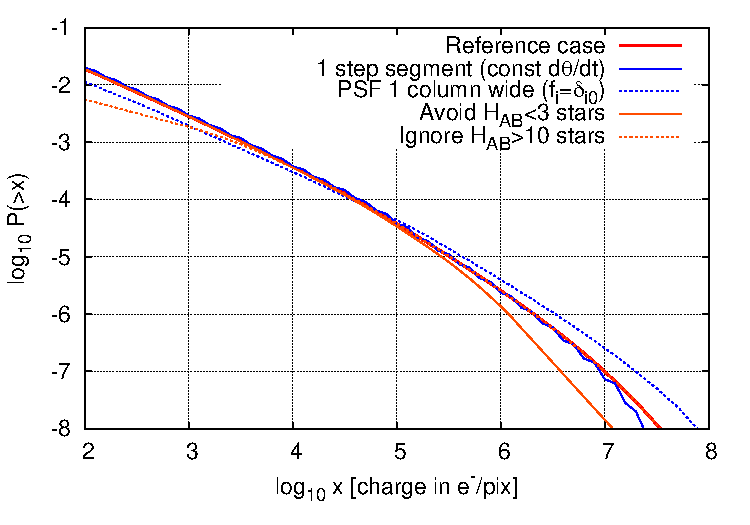
\includegraphics[width=5in]{Plots/slew_compare.pdf}
\caption{\label{fig:slewcompare}Comparison of stimulus levels predicted
under different assumptions and approximations. The vertical axis
shows the log probability to exceed a given stimulus level during a
slew of 0.4 degrees (a step along the short axis of the field,
executed frequently during the HLS). The thick red line indicates
reference assumptions. The solid blue line treats the slews as being
at constant $\dot\theta$. The dashed blue line approximates the PSF as
1 column wide (all the flux from the star is concentrated in the
central column). The orange lines show what happens if bright ($H_{\rm
AB}<3$) or faint ($H_{\rm AB}>10$) stars are excluded from the model.}
\end{figure}

\begin{figure}
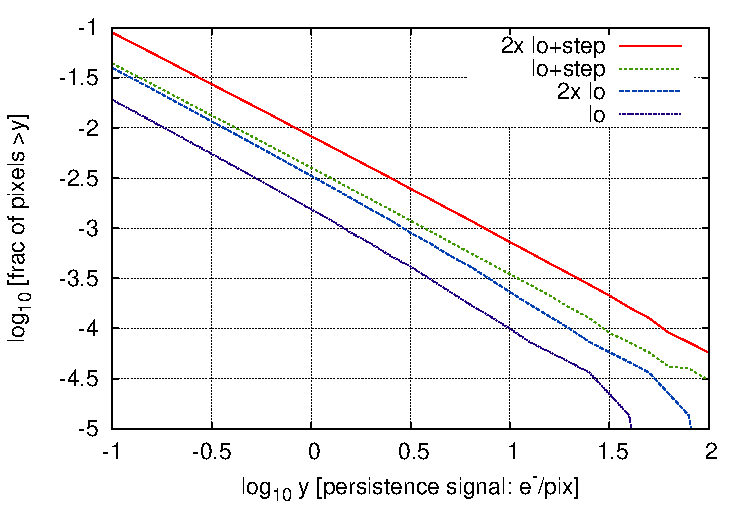
\includegraphics[width=5in]{Plots/sp_cdf.pdf}
\caption{\label{fig:sp_cdf}The cumulative distribution function of slew-induced persistence in the HLS imaging survey, $P(>y)$.
The persistence signal $y$ is estimated in electrons per pixel; the decaying persistence curve is integrated over a 160 s. Several persistence models are shown, including the ``lo'' case (typical of the development detectors), and a ``lo+step'' case (including an order of magnitude step at saturation, as seen in portions of some detectors). This figure has not been updated yet to go from the 6-year to the 5-year observing plan, although we expect only minor differences.}
\end{figure}

After negotiating with the Project, we settled on a mitigation strategy for slew persistence that involved saving the spacecraft orientation information from the Attitude Control System (ACS), using this to predict the locations of persistence from bright star streaks, and masking $\pm2\sigma$ on either side of these streaks. Unmasked streaks are simply accepted as part of the systematic error budget. Their impact on shape measurement is based on an analytic result derived by our SIT and tested against Monte Carlo simulations:
\begin{equation}
\Delta \gamma_1 + i\Delta \gamma_2 = \frac{M\Omega_{\rm
max}\sigma_{\rm n}^2 R^4}{2F^2N_{\rm ind}\,{\rm Res}} f_{\rm scale}
f_{\rm aniso},
\label{eq:dg}
\end{equation}
where $\Delta\gamma_{1,2}$ are the two components of spurious shear; $M$ is a margin factor; $\Omega_{\rm max} = 421.3$; $\sigma_{\rm n}^2$ is the variance of the persistence image; $R$ is the radius of the galaxy in pixels; $F$ is the signal from the galaxy in electrons per exposure; $N_{\rm ind}$ is the number of {\em independent} exposures of the galaxy\footnote{This may be less than the total number of exposures of the galaxy, since slew persistence from successive exposures will be correlated.}; Res is the galaxy resolution factor \cite{Bernstein2002}; $f_{\rm scale}$ and $f_{\rm aniso}$ are factors $\le 1$ describing the scale dependence and anisotropy of the persistence power spectrum (defined to be 1 in the worst case).

The results of this study -- shown in Figure~\ref{fig:slew_results_oct16} -- are promising, given the top-level systematic shear budget of $2.7\times 10^{-4}$ and that the modern detectors typically show ``lo'' or (in some regions) ``lo+step''-like behavior, rather than the much larger persistence characteristic of the WFC3-IR model (third column). The masking algorithm will continue to be revisited as part of the mission optimization. However, the small number of masked pixels led the FSWG to conclude that a dark shutter that operated during every slew was not required for the WFIRST HLS.

\begin{figure}
\includegraphics[width=5in]{Plots/slew_results_oct16.pdf}
\caption{\label{fig:slew_results_oct16}The outcome of the October 2016 slew persistence study. This shows the masked pixel fraction and the predicted systematic shear due to unmasked streaks as a function of both the persistence model and the accuracy of pointing information.}
\end{figure}

We carried out a related study, also using Eq.~(\ref{eq:dg}) and related machinery, to assess how well we need to know the dark current for WFIRST. Dark current measurements without a dark filter are possible, e.g.\ via median algorithms that combine many exposures from a survey, but are subject to: (i) a degeneracy in which the ``true'' sky brightness is unknown and hence the zero level of the dark current cannot be established, and (ii) possible correlated errors from imprinted celestial sources. The requirements, as derived in the appendix to the calibration plan, are:
\begin{list}{$\bullet$}{}
\item The error in the dark current + bias determination in a 140 s
HLS imaging exposure shall be no more than $0.0096f_{\rm corr}^{-1/2}$
e/p/s (uncorrelated part) or $0.0017 f_{\rm corr}^{-1/2}$ e/p/s
(imprinted celestial sources).
\item The error in the dark current + bias determination in a 297 s
HLS spectroscopy exposure shall be no more than $0.0059 f_{\rm
corr}^{-1/2}$ e/p/s (uncorrelated part) or $0.00072 f_{\rm
corr}^{-1/2}$ e/p/s (imprinted celestial sources).
\end{list}
Here ``$f_{\rm corr}$'' denotes the factor by which we plan to correct biases induced by errors in the dark current map (we normally choose $f_{\rm corr}=1$ to be conservative). The requirements are traceable to additive shear biases from non-circular imprinted celestial sources; multiplicative shear biases as the noise in the dark current map results in e.g.\ galaxy centroids getting ``pulled'' toward pixels whose measured dark current fluctuates below the true dark current of that pixel; and Eddington-like biases for sources detected in the GRS. While the semi-analytic estimates in the calibration plan based on source counts suggest that the HLS imaging requirement can be met without a dark filter, our SIT and the Calibration Working Group had concerns about possible degeneracies in the self-calibration procedure that can only be addressed by a detailed simulation. Moreover, the approach requires empty space in the images, which we will not have in the case of grism spectroscopy. As the imaging exposures are shorter than the spectroscopy exposures, this would require dedicated long imaging exposures (of HLS spectroscopy exposure length) just for the purpose of self-calibrating the dark. Due to sky Poisson noise, we would need many of these images -- our Feburary 2017 estimate was for $N=73$ exposures, which, if done every week, would consume 4\%\ of the wall clock time. In light of these and other issues, the Calibration Working Group recommended that WFIRST maintain the dark filter.

\subsubsection{Calibration plan}

Our SIT has contributed extensively to the WFIRST WFI Calibration Plan. This includes extensive quantitative analysis of proposed calibration techniques, as detailed in the appendix to the plan. Some highlights follow.

The requirement on knowledge of the dark current and the calibration approaches are fully defined, based on analysis done during the dark filter trade (October 2016 -- February 2017).

Weak lensing was found to place demanding requirements on measurement of the count rate-dependent non-linearity (CRNL). The weak lensing program is sensitive to CRNL because it enhances the bright center of a PSF star relative to its wings, thereby making the star appear slightly smaller, but does not have a similar effect on the faint galaxies used for shape measurement. The PSF second moment is biased by a factor of $1-\alpha$ (where $\alpha$ is the CRNL exponent), and has a top-line systematic error budget of $7.2\times 10^{-4}$. This means that if $\alpha$ is measured to $\pm 3\times 10^{-4}$ (the requirement from the supernova SITs), then CRNL consumes 17\%\ of the PSF size error budget, in an RSS sense. Given that CRNL is a pernicious bias for two of the dark energy probes, we recommended a multi-faceted approach to CRNL calibration, including a lamp-on/lamp-off capability for WFIRST (this was not available on WFC3-IR).

Our team has revisited the wavefront stability requirements for weak lensing, using a set of codes and scripts on the team's GitHub site. This begins with a Fisher matrix analysis of the uncertainties in the shear power spectrum, and our top-line requirement that the systematic errors be equivalent to the statistical errors even if the survey is extended to 10,000 deg$^2$ (i.e.\ in an RSS sense, the systematic errors should be 20\%\ of the statistical errors in the nominal 2,000 deg$^2$ survey). Requirements are assessed using the significance, defined by
\begin{equation}
Z = \sqrt{\Delta{\bf C}\cdot{\bf\Sigma}^{-1}\Delta{\bf C}},
\label{eq:alpha}
\end{equation}
which is the number of sigmas at which one could distinguish the correct power spectrum from the power spectrum containing a systematic error. We built sub-allocations for multiplicative (shear calibration) errors, and for additive (spurious shear) errors in each angular bin. An early discovery was that this process depends on the redshift dependence of the shear error: some redshift dependences are ``worse'' than others by the $Z$-metric. The worst possibility is {\em not} for the error to be redshift-independent, but rather for it to change sign, as this can mimic a change in redshift evolution of the growth of structure.

In our current formalism, for each angular template, we introduce a limiting amplitude $A_0^{\rm flat}(\alpha)$, defined to be the RMS spurious shear per component $A_0$ at which we would saturate the requirement on $Z(\alpha)$ for angular bin $\alpha$ in the case of a redshift-independent systematic $w_i=1\,\forall i$ (here $\alpha$ denotes an angular bin and $i$ a redshift bin). That is, if the additive systematics did not depend on redshift, we could tolerate a total additive systematic shear of $A_0^{\rm flat}$ (RMS per component) in band $\alpha$. We also introduce a scaling factor $S[{\bf w},\alpha]$ for a systematic error
\begin{equation}
S[{\bf w},\alpha] = \frac{Z(\alpha) \,{\rm for\,this\,}w_i}{Z(\alpha)\,{\rm for\,all\,}w_i=1}
\end{equation}
that depends on the redshift dependence $w_i$. An additive systematic error that is independent of redshift will have $S=1$. A systematic that is ``made worse'' by its redshift dependence will have $S>1$, and a systematic that is ``made less serious'' by its redshift dependence will have $S<1$. The requirement that the (linear) sum of $Z$s not exceed $Z(\alpha)$ thus translates into
\begin{equation}
\sum_{\rm systematics} [A(\alpha)]^2\times S[{\bf w},\alpha] \le [A_0^{\rm flat}(\alpha)]^2,
\label{eq:A-S-sum}
\end{equation}
where $A(\alpha)$ is the RMS additive shear per component due to that systematic. We take the ``reference'' additive shear to be the additive shear in the most contaminated redshift slice; in this case, $w_i=1$ for that slice, and $|w_i|\le 1$ for the others. Under such
circumstances, we can determine a {\em worst-case scaling factor} $S_{\rm max,\pm}(\alpha)$, which is the largest value of $S[{\bf
w},\alpha]$ for any weights satisfying the above inequality. We may also determine a worst-case scaling factor $S_{\rm max,+}(\alpha)$
conditioned on $0\le w_i\le 1$, i.e.\ for sources of additive shear that have the same sign in all redshift bins. In most cases, however, something is known about the redshift dependence of the systematic error (e.g.\ for PSF errors the error scales with the size of the galaxy, and hence has a redshift dependence tied to the measured redshift evolution of galaxy sizes). In these cases, we use the correct redshift weighting factor $S$. This approach has been critical in order to set stability requirements that are consistent with the Project's integrated modeling results.

We have begun incorporating the HLS observing strategy (\S\ref{sec:operation}) in studies of self-calibration of time-dependent drifts in the response of the system (i.e.\ time dependence of the conversion from $\mu$Jy on the sky to DN/s in the digitized detector system outputs). This model is in a state of flux as we add parameters to it, but here we show a current snapshot allowing for time-dependent drifts of the response of each of the 18 SCAs making up the focal plane, with time dependence parameterized in calibration periods of $\Delta t$ (assessed down to a period of 3 hours) each. Both individual-SCA drifts and common-mode drifts are allowed, with an assumed intrinsic variation (calibration prior) of 1\%\ RMS drift in each $e$-fold of timescales. A network of randomly distributed stars with a density of 500 stars/deg$^2$ and $S/N=50$ was assumed; in self-calibration, the magnitudes of these stars are {\em not} known a priori, but are assumed to be stable across multiple repeated observations of the same field. These are preliminary parameters being used to test our tools and are not currently held as requirements. The stellar density model is very conservative since the Trilegal model predicts star counts of 572, 803, 990, and 1137 stars/deg$^2$ at $H_{\rm AB}=18-19$, $19-20$, $20-21$, and $21-22$ at the SGP, and even an $H_{\rm AB}=22$ star will have $S/N>50$. The temporal stability of the system needs further study and will be varied as an input parameter in future versions of this model. The current model uses the April 19, 2017 update to the HLS observing strategy. The number of calibration parameters varies depending on the filter, since there are no parameters for periods of time when the instrument is not observing in that filter; the current version has 17262 parameters for the H band.

Despite the intrinsic stability assumed, in which each SCA can have its response fluctuate by 1.67\%\ RMS from one time interval to the next, the repeated observations do an excellent job of tracking these changes and reducing the posterior uncertainty. Even for $\Delta t = 0.125\,$days$=3\,$hours, the posterior calibration errors are at the level of 0.14--0.17\%\ RMS (here ``RMS'' is weighted by number of observations), depending on the filter.  An example of the model output (predicted uncertainties in the calibration parameters for each SCA at each epoch) is shown in Figure~\ref{fig:hcalfig}. It must be remembered that this analysis is overly simplistic in some ways -- particularly that we have not yet allowed for shorter-timescale variations (i.e.\ on timescales $<\Delta t$), nor have we allowed for separate gain drifts among the different readout channels. These will have to be included in a future version of the model. On the other hand, the stellar density and $S/N$ assumptions were extremely conservative (e.g.\ the full range of stellar magnitudes 18--22 should have 7 times more stars than were assumed, even at the Galactic pole), so there is margin to absorb these additional degrees of freedom. The next iteration of the model for time-dependent calibration drifts will include additional parameters, as well as updated priors reflecting expected detector system stability rather than the place-holder requirements shown here.

\begin{figure}
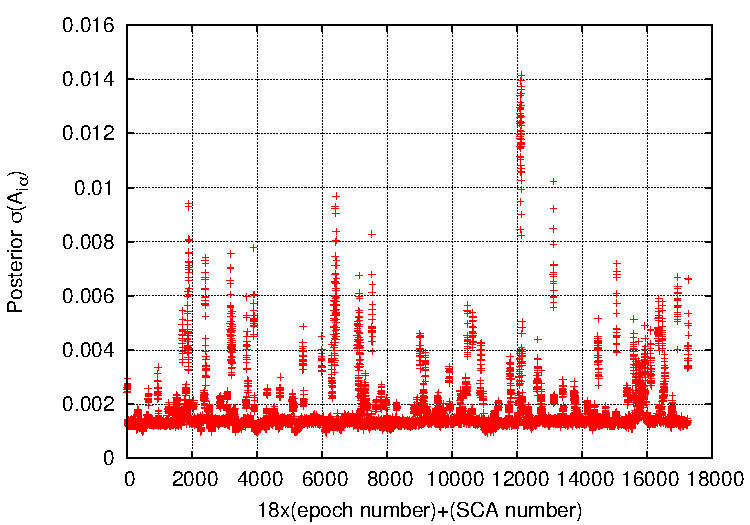
\includegraphics[width=4.5in]{Plots/hcalfig.pdf}
\caption{\label{fig:hcalfig}An example of the posterior calibration error from an HLS self-calibration calculation. The horizontal scale displays the time intervals (left-to-right in time order), with 18 points per time interval indicating the various SCAs. The vertical axis shows the standard deviation of the calibration solution for that SCA at that time, $\sigma(A_{i\alpha})$, relative to the survey mean. The figure shows the case of H band with $\Delta t = 0.125$ days. This example had 17262 calibration parameters. A few epochs, mostly containing only a few observations, are poorly constrained due to minimal overlap observations. It is subject to refinement and the input parameters of the model will be varied as we work toward requirements on the stability of the detector system.}
\end{figure}

\subsubsection{Detector characterization}

The WFIRST dark energy analyses will place enormous demands on our understanding of the detectors. Some aspects of this problem can be anticipated in advance -- for example, we know that effects such as inter-pixel capacitance, count-rate-dependent non-linearity, etc.\ will need to be carefully characterized, and we are working as part of the Calibration Working Group to build these measurements into the mission. However, with systematic error budgets at the level of a few$\times 10^{-4}$, it is likely that WFIRST analyses will turn up new effects that were not apparent in past missions. Therefore a key task for our SIT is to analyze the data from development detectors and identify these new effects early enough to inform the calibration plan.

In ground-based weak lensing projects using thick CCDs (e.g.\ DES), one of the key detector issues has been the {\em brighter-fatter effect} (BFE). This is an electrostatic effect in which as a pixel fills up with collected charge, it changes the electric field geometry and new charges generated are more likely to be deflected into neighboring pixels. This has the effect of making bright stars appear larger than faint stars, as the repulsion effect is non-linear and increases with signal level. The field geometry is very different in a NIR detector, but a brighter-fatter effect is still possible.

We have searched for the brighter-fatter effect in the H4RG detector arrays using the flat fields for two devices H4RG-17940 and H4RG-18237, provided to us by the DCL. The BFE imprints a signature in the auto-correlation function of a flat field; using the correlations in multiple non-destructive reads in a flat field, one can separate linear IPC from the BFE. Preliminary brighter-fatter effect results for H4RG-17940 are shown in Figure~\ref{fig:kernel}. The BFE coefficients are $a'_{\Delta i,\Delta j}$, which is the fractional change in effective area of pixel $(i,j)$ when an electron is placed in pixel $(i+\Delta i, j+\Delta j)$; they have units of parts per million per electron (ppm/e). The flat auto-correlations are sensitive to both the brighter-fatter effect and non-linear inter-pixel capacitance (NL-IPC); we are currently working on distinguishing the two effects.

\begin{figure}
\includegraphics[width=6.2in]{Plots/kernel-17940B.pdf}
\caption{\label{fig:kernel}The BFE + NL-IPC coefficients $[K^2a'+KK']_{\Delta i,\Delta j}$ (left panel) and IPC-corrected coefficients $a'_{\Delta i,\Delta j}$ (right panel), for H4RG-17940. Note that the IPC-corrected coefficents assume that the IPC is linear, i.e.\ the non-overlapping correlations are ascribable entirely to the BFE and not NL-IPC. The $1\sigma$ uncertainty in each pixel is 0.07 ppm/e.}
\end{figure}

\subsection{Photometric Redshifts}
\label{sec:wl_calibration}

\begin{figure} 
\centering
 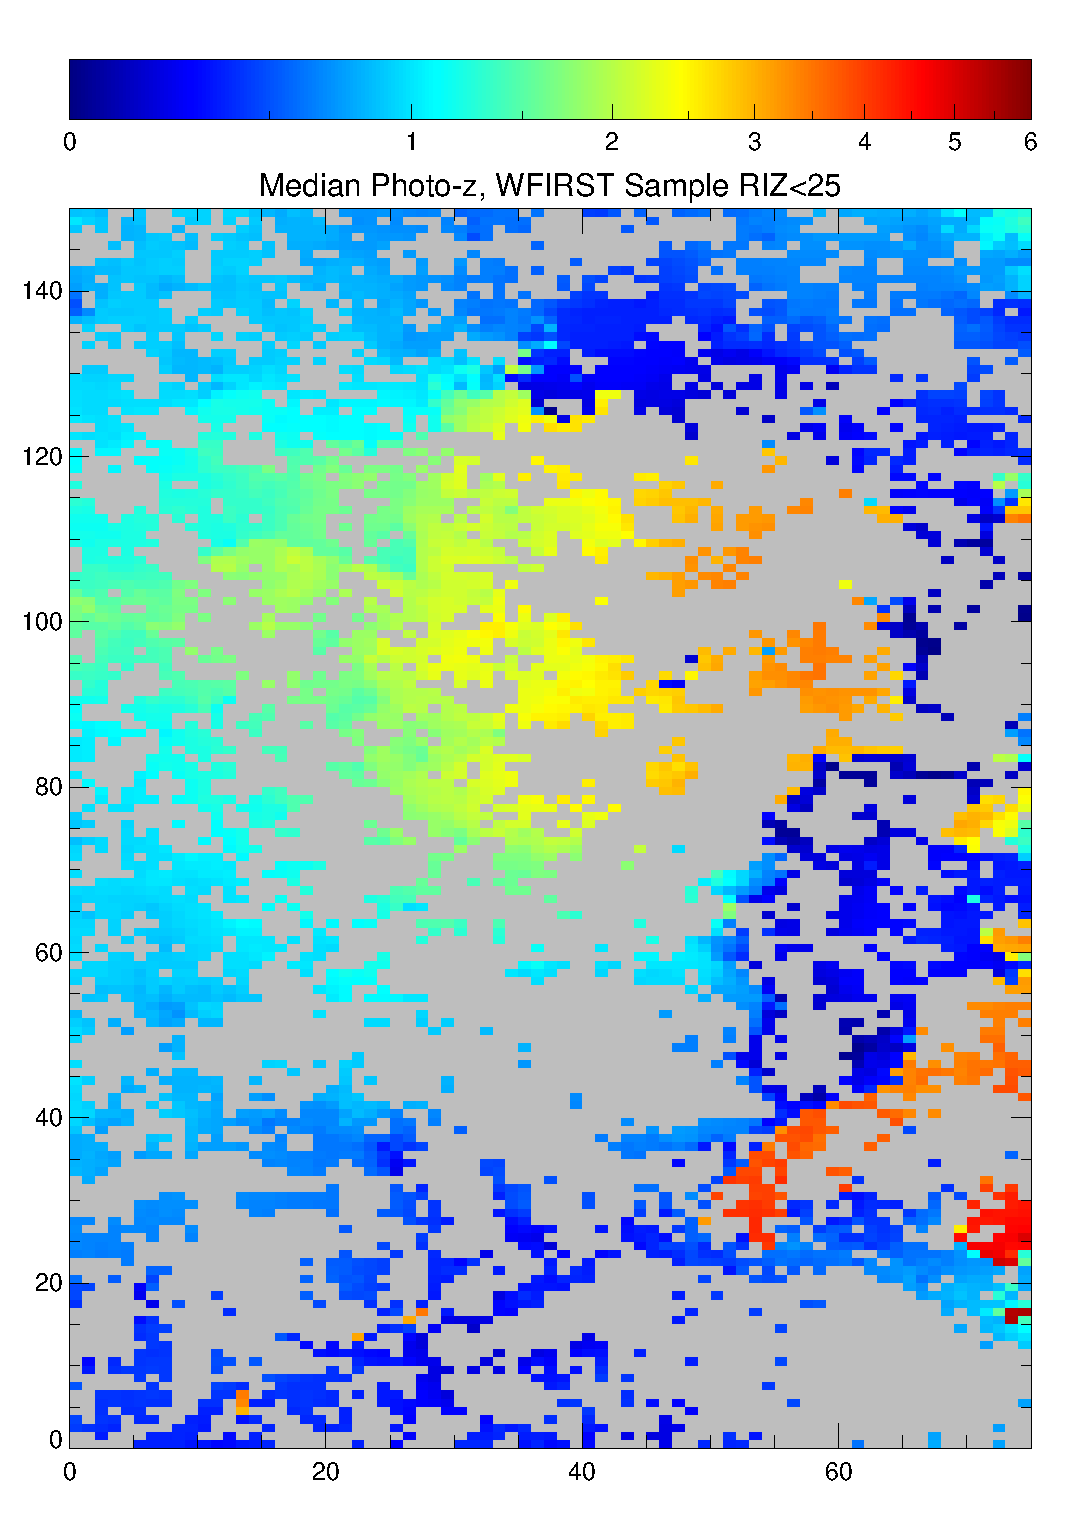
\includegraphics[width=0.45\textwidth] {./plots/wfirst_color_dist.eps}
\caption{A Self Organizing Map (SOM) \citep{Masters2015} of color space generated from $\sim6$ square degrees of data in the VVDS 2h, SXDS/UDS, COSMOS, and EGS survey areas colored by photometric redshift is shown.  Only regions occupied by the CANDELS survey are colored, with the remaining area grey.  CANDELS only covers 42\% of the color space, representing 49\% of the overall galaxy population.  }
\label{fig:EuclidCandelsRep}
\end{figure}

 In the first year of SIT activity we have focused on developing accurate data-driven simulations of the WFIRST lensing galaxy population and determining potential methods to calibrate this sample.  The closest analogs to WFIRST data are the COSMOS and CANDELS HST surveys, however neither is fully analogous to WFIRST HLS data.  The COSMOS data cover 1.7 square degrees with HST-ACS (F814W) with ground based data analogous to LSST.  However, WFIRST analogous infrared data are not available over the majority of the field and extrapolations to the WFIRST lensing cuts from the F814W data over-estimate the number-density of sources usable for lensing.  In contrast, CANDELS has WFIRST analogous infrared data, but covers only 0.2 square degrees,which means it does not sample the full WFIRST galaxy population, and has very heterogeneous optical coverage.  Specifically, a comparison between the CANDELS and COSMOS data to R,I,Z$<$25 found that only 42\% of COSMOS galaxy colors (representing 49\% of the galaxy population) are present in CANDELS.  Figure \ref{fig:EuclidCandelsRep} shows a Self Organizing Map (SOM) \citep{Masters2015} of the galaxy color space with regions where CANDELS galaxies fall marked.  The empty regions are shown in grey and correspond to cells with low galaxy density in COSMOS.  So these galaxies are simply less likely to be found in the relatively small area of CANDELS. 


To overcome these limitations we have taken several approaches.  First, we have collected a homogeneous 0.3-2.5$\mu$m data set over $\sim6$ square degrees in the VVDS 2h, UDS/SXDS, COSMOS, and EGS fields.  These data are not as deep as WFIRST, but are analogous to the LSST and Euclid data and allow us to estimate the cosmic variance in galaxy population and estimate requirements on spectroscopy.  These have been combined with the CANDELS catalogs which probe WFIRST depth but are sample size and variance dominated.  We then adapted the simulations described in \citet{stickley2016} developed for the SPHEREx mission to assign a R$\sim$600 spectra to each object.  The CANDELS data are very heterogeneous (see Table \ref{tbl:filters}), so we converted the various photometric systems to a LSST+WFIRST system.  Figure \ref{fig:filters} shows an example of the LSST+WFIRST system along with the CANDELS filters on GOODS-S as an example.  For the conversion we compared the converted photometry from other bands to actual CFHT-LS $u^*$, $g^*$, $r^*$, $i^*$, $z^*$ and VISTA $Y$, $J$, $H$, $K_s$ photometry in fields where they are available.   We found a simple linear interpolation between filters in flux produced the best agreement.  Using the \citet{stickley2016} or other template fits produced discretized value  in the output fluxes which biased further analysis.  




\begin{figure} 
\centering
  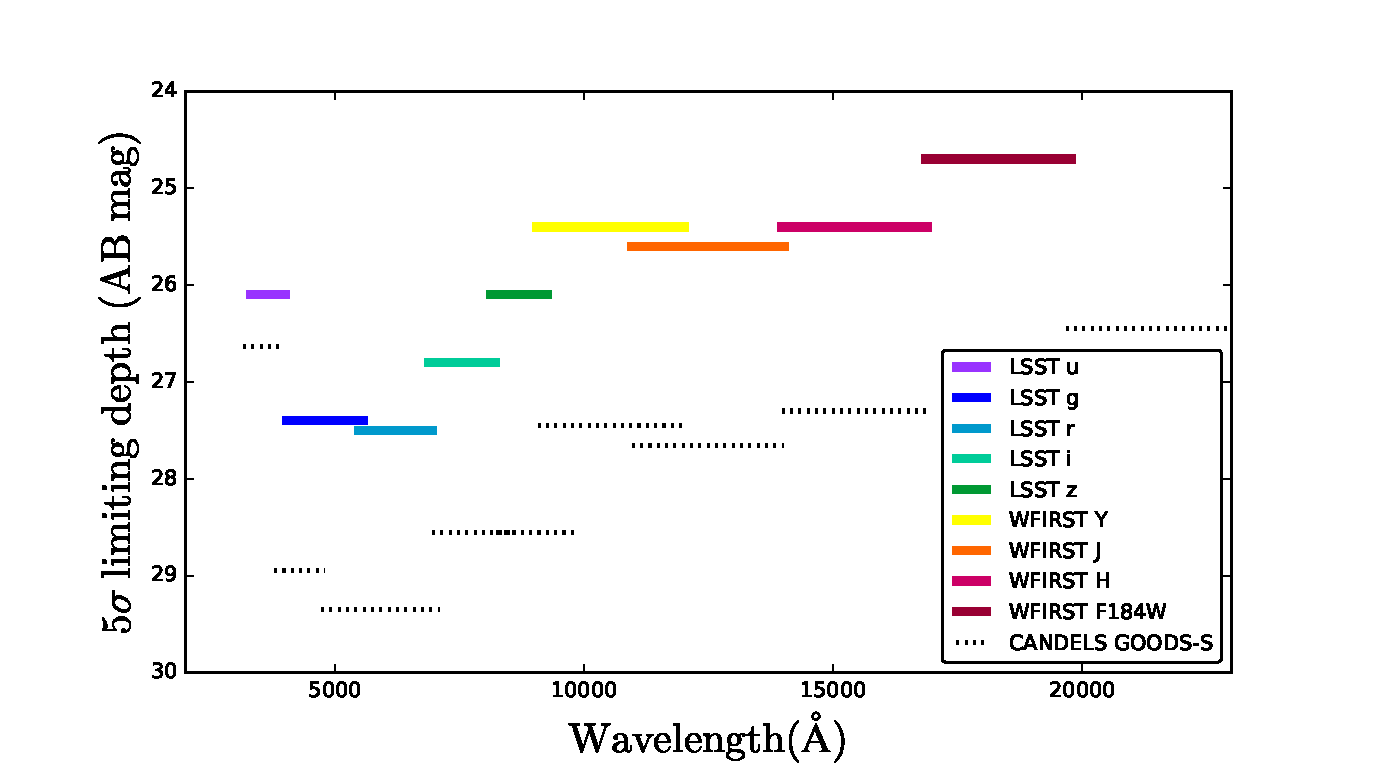
\includegraphics[trim=0cm 0cm 0cm 0cm, clip,width=0.50\textwidth] {./plots/filters.eps}
\caption{The 5$\sigma$ limiting AB magnitude of LSST and WFIRST filters plotted as solid color lines and the 5$\sigma$ limiting AB magnitude of CANDELS GOODS-S filters are plotted with dotted black lines (see Table \ref{tbl:filters} for filter names).  Note the significant differences in the filter system which necessitates conversion from one to the other. }
\label{fig:filters}
\end{figure}


The combination of these catalogs produces a reasonable estimate of the WFIRST galaxy population for the purposes of assessing variance and the effects of cuts.  However for some analysis a fully simulated catalog is required so that the inputs are known perfectly.  To provide this we further adapted the methods described in \citet{stickley2016} to produce simulated WFIRST+LSST photometry.  These three sets of simulated samples are being provided to other WFIRST SIT teams for their analysis. Specifically we have been working with the Foley SNe team to simulate photo-z performance for supernova cosmology. 

\begin{table*}
\footnotesize
\centering
\caption{CANDELS filters in each field used to create the LSST+WFIRST catalog}
\begin{tabular}{*{15}{c}}
\hline
\hline
\\
Field&&&&&&& Filters\footnote{\footnotesize Refer to CANDELS catalog papers for detailed description of observations in each filter, GOODs-S: \citealt{Guo2013}; GOODS-N: Barro et al. in prep; EGS: \citealt{Stefanon2017}; UDS:\citealt{Galametz2013}; COSMOS: \citealt{Nayyeri2017}}&&\\
\\
\hline
\\
GOODS-S& $\rm U_{VIMOS}$& $\rm F435W$& $\rm F606W$&$\rm F775W$ & $\rm F814W$ & $\rm F850lp$ & $\rm F098W$& $\rm F105W$ & $\rm F125W$ &$\rm F160W$&$\rm Ks_{HAWK-I}$\\
\\
GOODS-N&$\rm U_{KPNO}$& $\rm F435W$& $\rm F606W$&$\rm F775W$ & $\rm F814W$ & $\rm F850lp$ &$\rm F105W$ & $\rm F125W$ &$\rm F160W$& $\rm Ks_{CFHT}$\\
\\
EGS& $\rm U_{CFHT}$& $\rm g_{CFHT}$& $\rm F606W$ &$\rm r_{CFHT}$& $\rm i_{CFHT}$& $\rm F814W$ &$\rm z_{CFHT}$ & $\rm F125W$&$\rm F160W$&$\rm Ks_{CFHT}$\\
\\
UDS& $\rm U_{CFHT}$& $\rm B_{subaru}$&$\rm F606W$ &$\rm Rc_{subaru}$& $\rm i_{subaru}$&$\rm F814W$ &$\rm z_{subaru}$ & $\rm Y_{HAWK-I}$&$\rm F125W$&$\rm F160W$&$\rm Ks_{HAWK-I}$\\
\\
COSMOS&$\rm U_{CFHT}$& $\rm B_{subaru}$& $\rm F606W$&$\rm r_{subaru}$&$\rm i_{CFHT}$&$\rm F814W$ &$\rm z_{CFHT}$ & $\rm Y_{UVISTA}$&$\rm F125W$&$\rm F160W$& $\rm Ks_{UVISTA}$\\
\\
\hline
\end{tabular}
\label{tbl:filters}
\end{table*}


\begin{figure} 
\centering
\includegraphics[trim=0cm 0cm 0cm 0cm, clip,width=0.95\textwidth] {./plots/histogram_wfirst_notEuclid.png}
\caption{{\bf Left:} A magnitude histogram of the WFIRST lensing sample split into a C3R2 Euclid like lensing sample (blue, $RIZ<25$) and those only in WFIRST (green).  Roughly 20\% of the WFIRST sample consists of galaxies fainter than what C3R2 is calibrating for Euclid.  Note the Euclid lensing sample is cut at $RIZ<24.5$, shallower than the proposed calibration \citep{Masters2015}.  {\bf Right:} The redshift distribution of the C3R2-Euclid sample (blue) and the WFIRST only sample (green) are shown normalized to an integral of 1. Even though the WFIRST galaxies are fainter than the calibration limit they cover a redshift range similar, just with with more galaxies at high-redshift.   }
\label{fig:EuclidVsWFIRST}
\end{figure}

\begin{figure} 
\centering
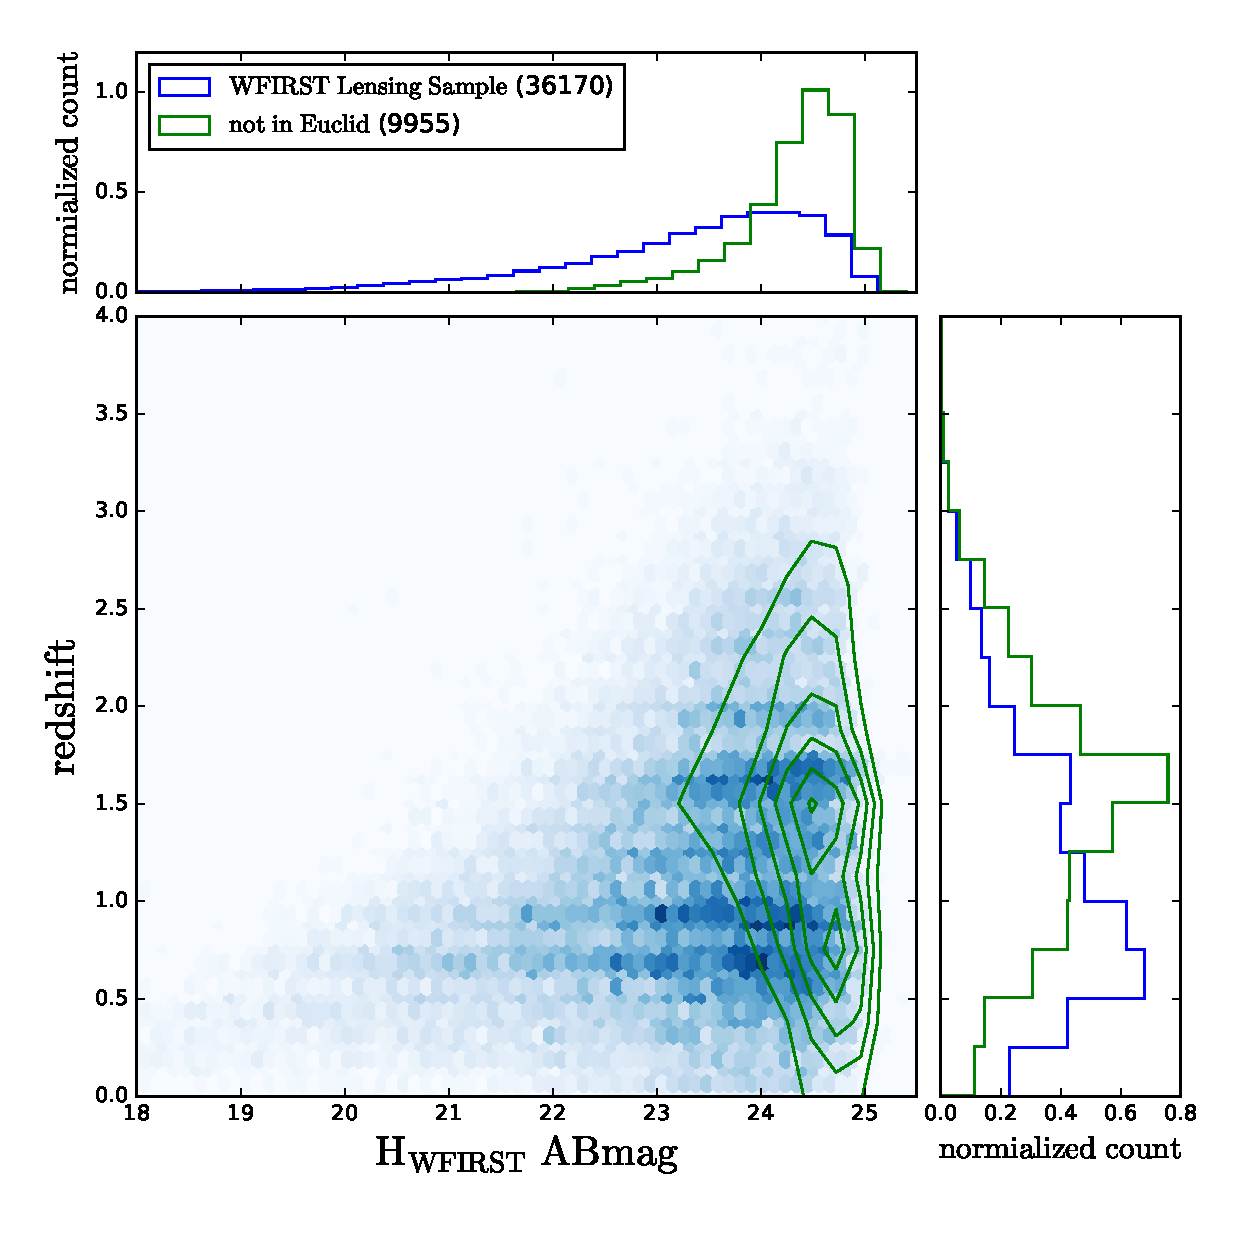
\includegraphics[trim=0cm 0cm 0cm 0cm, clip,width=0.95\textwidth] {./plots/redshift_magnitude.eps}
\caption{$H$ band magnitude vs redshift is plotted for the WFIRST lensing sample shown in Figure \ref{fig:EuclidVsWFIRST} with shading indicating relative density.  The WFIRST only sample shown as green contours and the histograms from from Figure \ref{fig:EuclidVsWFIRST} are plotted on the axis.   }
\label{fig:EuclidVsWFIRST2}
\end{figure}

These simulations have been used for several analyses for the WL SIT.  Figure \ref{fig:EuclidVsWFIRST} shows the relative differences in the magnitude and redshift distribution of the total Euclid and WFIRST faint lensing samples.  WFIRST clearly adds fainter and higher-redshift systems to the weak lensing sample.  However, Figure \ref{fig:WFIRSTSOM} shows a Self-Organizing-Map analysis \citep{Masters2015} of the WFIRST lensing sample compared with the Euclid sample. Even though WFIRST is significantly fainter than Euclid, 96\% of galaxies fainter than the Euclid sample have color analogs at brighter magnitudes.  The implication is that while WFIRST is seeing fainter galaxies than Euclid, these galaxies are very similar to less numerous but brighter systems seen by Euclid.

\begin{figure} 
\centering
 \includegraphics[trim=0cm 0cm 0cm 0cm, clip,width=0.98\textwidth] {./plots/SOM_WFIRST_EUCLID.png}
\caption{A Self Organizing Map (SOM) \citep{Masters2015} of the WFIRST color space based on the CANDELS data cut to the WFIRST lensing sample color coded by their median redshift.  The left panel shows SOM cells that contain galaxies too faint to be in the C3R2 RIZ$<25$ Euclid like sample \citep{Masters2015,Masters2017}.  The right panel shows SOM cells with galaxies that are in the C3R2 sample.  $\sim96\%$ of the WFIRST color space is occupied by galaxies in the C3R2 sample, however $\sim20\%$ of the WFIRST sample is fainter than the C3R2 limit.  This means their calibration would have to be verified to ensure no magnitude dependence on redshift. }
\label{fig:WFIRSTSOM}
\end{figure}

To determine how difficult it would be to obtain spectra for these faint systems we conducted an analysis of the R$\sim$600 SEDs fit to the photometry.  Based on the C3R2 survey spectra \citep{Masters2017} we developed a spectral simulator which accurately re-produces ground based spectra for Keck DEIMOS, LRIS, and MOSFIRE.  In addition to these instruments the simulated response of the WFIRST-IFC was simulated.  Example simulated spectra based on the model fits along with actual Keck spectra obtained for those sources are shown in Figure \ref{fig:SpecSim}.  

\begin{figure} 
\centering
 \includegraphics[trim=0cm 0cm 0cm 0cm, clip,width=0.45\textwidth] {./plots/realspec.png}\\
  \includegraphics[trim=0cm 0cm 0cm 0cm, clip,width=0.45\textwidth] {./plots/simspec.png}

\caption{ A real (top) and simulated (bottom) spectra of a $I=22.7$ galaxy in the C3R2 sample.}
\label{fig:SpecSim}
\end{figure}

We found that indeed most of the faint WFIRST lensing galaxies were analogs of brighter systems. This alleviates the need to obtain spectroscopic redshifts to this population since the color-redshift relation will be known.  However, steps must be taken to validate that the redshift distribution does not change at fainter magnitudes in ways not apparent in the WIFRST+LSST colors. 

The simplest method would be to extend a survey such as C3R2 \citep{Masters2017} to fainter magnitudes. However, these faint galaxies are difficult to obtain high-quality spectra for from the ground.  For the purposes of this analysis we define high quality as an SNR$>$7 on two emission features or an SNR$\sim5$ on an underlying continuum.  Based on this criteria, 20\% of the WFIRST color space requires $>5$h spectra from Keck.  It is important to note this is in terms of color space, and the exact number of spectra required to calibrate this color space will require further analysis.   Of these, 1\% are sources that require long ground exposures due to strong emission lines falling between ground based observing windows and spectra could be obtained with the WFIRST grism.  A further 15\% would have high-quality redshifts with WFIRST-IFC parallel observations based on simulating the spectra and assessing the number of features with SNR$>$7.  However, due to the low-resolution of the WFIRST-IFC further analysis may be merited.   The remaining 4\% of galaxies could not be calibrated by WFIRST or from the ground with 10m telescopes and would require either ELTs or JWST.


%{\bfseries C.H.: Need uniform ``primary/secondary/tertiary'' nomenclature. Also discuss photometric calibration requirements.}

%\subsection{Cosmological Forecasting, Methodology Development, and Cosmological Simulations}
\subsection{Cosmological Forecasting, Simulations, and Methodology Development (D2, D8, D9)}
\label{sec:wl_methodology}
%=========================================================================
%\Auth{David W, Tim, Elisabeth, Rachel B, Alina, Bhuvnesh}


\subs{Forecasting.}
Cosmological forecasting plays
an essential role in connecting strategies and requirements defined at
the instrument and observation level to WFIRST's top-level science goals.
Co-Is Bean, Hirata, Padmanabhan, Wang and Weinberg have been
involved in the forecasting for the WFIRST reports and
for cosmological surveys and space missions in general.
One of our early activities will be to develop a forecasting
framework for WFIRST building on Eifler \& Krause's \CoLi, incorporating all of the dark
energy probes from the HLS Imaging, Spectroscopy, and Supernova surveys.
We will incorporate the impact of the leading observational and theoretical systematics
through ``nuisance parameters'' that can be marginalized over in cosmological
parameter estimates.  This framework will be much more thorough
than the one used for the SDT reports, and it will enable complete
flow-down and flow-up analyses between the instrument, strategy, and
software requirements and the expected cosmological performance of
WFIRST.  We will initially use analytic approximations for error covariance
matrices and the dependence of observables on model parameters.  We will
steadily update these approximations using the simulations described below.
For cosmic shear, we will extend existing work on the WL bispectrum
(e.g., \cite{Kayo2013,Fu14}), which should
produce complementary constraints to the power spectrum and may have
similar statistical power given the high source density expected in
HLS Imaging.  Figure~1 illustrates the application of \CoLi\ to WFIRST
multi-probe forecasting.

\subs{Cosmological simulations.} As emphasized in SDT15, WFIRST will improve the statistical precision
of cosmic expansion and structure growth measurements by factors of $5-50$
compared to current data, and will require commensurate improvements in modeling the
lensing and clustering signals  and the astrophysical contaminants thereof.
We will  devote significant effort to modeling the nonlinear regime via a combination of numerical
simulations, perturbation theory, and empirical measurements, to
 address issues such as baryonic effects on matter clustering
\citep{Zentner2013,VanDaalen2014}; the
validity of the Born approximation \citep{Schafer2012}; and galaxy intrinsic
alignments \citep{Hirata2004,Laszlo2011,Krause2015}.
We will develop analysis strategies that take advantage of
our methodological improvements and marginalize over remaining uncertainties.
The computational requirements for cosmological simulations will increase
significantly in the years just prior to launch. Where these resources will
be sourced from is currently an unsolved issue that is being investigated at
the project level. Co-I Kiessling has been part of this effort at the request of
the project and she will be responsible for leading
the team efforts to quantify computing requirements beyond FY20.
% and to develop techniques to reduce them.
%
% RM took a bunch of long specific sentences and made this more general one.
%For cosmic shear, we will develop
%``self calibration'' strategies to eliminate biases and mitigate statistical
%losses from uncertainties in shear calibration and \photoz\ error
%distributions.  These strategies will be developed in concert with
%and informed by the methods and tests discussed previously in
%\S\ref{sec:wl_requirements} and~\ref{sec:wl_methodology}.
%We will use cosmological N-body simulations and hydrodynamic
%simulations to predict non-linear matter clustering at the accuracy
%needed for WFIRST modeling, including the impact of realistic
%treatments of baryonic physics (see, e.g., \cite{Zentner,VanDaalen,Etc}).
%We will apply ray tracing to cosmological simulations to test
%for biases such as due to the ``Born approximation'' typically used in weak
%lensing analysis, and to calibrate any necessary corrections.
%We will use hydrodynamic simulations, perturbation theory calculations,
%and empirical information to sharpen predictions of galaxy intrinsic alignment,
%one of the main theoretical systematics for cosmic shear.

%\textbf{Bhuv: The two paras below describe a very broad program. If not essential, perhaps better to make it shorter and less sweeping. Also, is the connection to image simulations ok?}
%Our methodology development and tests will make heavy use of cosmological
%simulations.
Most of our work will use large-volume $N$-body simulations (gravity only) in concert
with statistical recipes or semi-analytic models for assigning
galaxies to dark matter (sub-)halos. A large set of such simulations ranging in size from tens of billions to a trillion particles already exists. These will be made available to the collaboration by collaborator Heitmann and will be augmented over time with more simulations as needed.
We will use hydrodynamic simulations
of smaller volumes, provided by collaborator Yoshida, for targeted investigations such as the impact of
baryonic physics on the matter power spectrum or as a realistically
complicated test of non-linear galaxy bias models.
From the $N$-body simulations we will produce mock galaxy catalogs
both in fixed redshift cubes and in light cones with realistic survey
geometry and redshift evolution.
We will use these mocks to understand the effect of observational complications
(survey geometry, variable depth and completeness, etc.) on WL and clustering
measurements and to provide realistically clustered inputs for the pixel-level
simulations described earlier.

% C.H. -- I would really like this but it's very ambitious and not clear that it is
% higher priority than subsets of the HLS simulated at very high fidelity.
% By the end
%of the 5-year investigation period, we aim to produce several complete
%realizations of the full pixel-level HLS data set.

%The overall cosmological simulation effort is large, but many ambitious
%dark energy experiments face a similar challenge.
Our team includes
Co-I Kiessling and collaborators (Heitmann, Takada, Yoshida) who are leading similar efforts
for Euclid, Subaru HSC and PFS, DES, DESI and LSST. In \S
\ref{sec:fac_equip} we describe the computing facilities that will
enable these computations.
%By 2020, advances in computing will make it possible to run larger numbers of simulations, or explore more parameter space at a given size and resolution.
We will publish papers documenting our methodology development and
will simultaneously release the associated simulations.
This growing library of publicly available simulations will encourage
the broader community to develop analysis strategies that will
ultimately be applied to WFIRST (and other surveys).
%While we expect major advances over
%the 5-years of this SIT, we do not expect to solve all of the modeling
%challenges in this period.  One of our deliverables will be a list of remaining (post-CDR) tasks
%to address the remaining modeling uncertainties.

%\setlength\intextsep{-2pt}
%\begin{center}
%\begin{wrapfigure}{r}{1.0\textwidth}
\begin{figure}[!t]
 \begin{boxedminipage}{1.0\textwidth}
 \begin{center}
\includegraphics[width = \textwidth]{Plots/WFIRST_combi_forecasts.pdf}
\label{fig:WLsys}
 \end{center}
\vspace{-1.25cm}
\caption{\footnotesize{\CoLi\ forecasts of constraints on the dark energy equation-of-state
from combining current CMB+BAO+Supernovae (SN) data with anticipated WFIRST WL, GGL, projected clustering, cluster number counts, and cluster weak lensing measurements.
We adopt a flat universe with a DE equation of state
$w(z)=w_0+w_a[1-(1+z)^{-1}]$, with the $x-$axis showing the
value of $w$ at the pivot redshift ($z_p$) where it is best constrained by this data combination.
The left panel shows the improvement from WFIRST imaging data with statistical errors only.
In the middle panel, red contours show the effect of an uncorrected shear calibration error
of magnitude 0.004, while blue contours show the result with the same calibration error
after marginalizing over five shear calibration nuisance parameters with Gaussian priors of
width 0.002. The right panel shows a similar example for an astrophysical systematic,
the presence of galaxy intrinsic alignments (see \cite{Krause2015} for details). In both cases, marginalization removes the systematic error without significantly increasing the statistical uncertainty.
}}
%\begin{center}
\end{boxedminipage}
\end{figure}
%\end{wrapfigure}
%\setlength\intextsep{0pt}

\subs{Galaxy-galaxy lensing.} The combination of GGL with galaxy clustering
is an alternative route to extracting cosmological constraints from
an imaging survey.  Systematics are significantly different from those
affecting cosmic shear analysis, and theoretical studies suggest that
the statistical power is comparable \cite{Yoo2012}.  The need to mitigate systematics
favors a joint modeling approach to cosmic shear, GGL, and galaxy clustering,
which requires devising and testing models of non-linear galaxy
clustering and its dependence on redshift, building on studies such as
\cite{Yoo2006,Baldauf2010,Cacciato2013,Mandelbaum2013,Coupon15,More2015,Zu2015} and
including the possible impact of ``assembly bias'' connected to halo
formation histories.
We will include GGL in our cosmological forecasting framework
and identify any GGL-specific requirements distinct from those
tied to cosmic shear.

\subs{Clusters.} Our efforts in cluster analysis methodology will parallel those for
cosmic shear and GGL, facing many of the same issues but in the
(somewhat simpler) high mass halo regime. Co-I Weinberg
will lead the cluster effort with support from collaborators Rozo and
von der Linden.  While the WFIRST data set presents some
unique issues, we will draw extensively on the machinery being developed for
DES by Rozo, which follows the broad strategy laid
out in chapter 6 of \cite{Weinberg2013}, and for LSST, described in \cite{LSSTDESC12}.

The first branch of the cluster effort will focus on the identification
and characterization of clusters in WFIRST+LSST (or WFIRST+HSC) imaging.
This optical+NIR combination will lead to the best statistical precision,
since optical/IR selection can select clusters (at typical redshifts
$z \sim 0.5-1.5$) down to mass thresholds significantly lower than
X-ray or Sunyaev-Zeldovich detection; we expect $\sim 40,000$ clusters in the HLS
with masses $>10^{14}M_\odot$.
Building on DES methodology
\cite{Rykoff2014}, we will design and test (in simulations) prototype cluster finders for
WFIRST+LSST data.
Among the issues we will address are: completeness and contamination
of the cluster catalogs as a function of redshift and richness; biases
in estimated richness or cluster redshift; expected scatter between
richness and halo mass; accuracy of galaxy photometry in cluster regions;
accuracy of shear measurement in cluster regions; reliable separation
of foreground, member, and background galaxy populations for weak
lensing analysis; and ellipticity- or orientation-dependent
cluster selection.

A second branch recognizes WFIRST's unique potential for calibrating
cluster mass-observable relations at $z\gtrsim1$ via weak lensing.
Cluster-galaxy lensing (CGL, e.g.,
\cite{Sheldon2009,VonDerLinden2014}) is the method of choice for all
cluster surveys overlapping weak-lensing surveys, but requires
sufficient number densities of galaxies behind the clusters with
accurate photo-$z$s.  For cluster mass calibration at $z\gtrsim1$,
space-based shear measurements and photo-$z$s from the combination of
LSST and deep NIR photometry, such as delivered by WFIRST, are
therefore necessary. Calibrating cluster mass-observable relations
furthermore benefits tremendously from the availability of
multi-wavelength mass proxies (e.g. \cite{Wu2010}), hence we will
consider the synergies with X-ray (eROSITA) and SZ (Planck, AdvACT,
SPT-3G, CMB-S4) measurements, with special attention to the impact on
survey footprint placement.  We will also investigate the potential for HLS-CMB cross-correlations to extract the kinetic Sunyaev-Zeldovich signature to constrain dark energy, gravity and and neutrino mass sum \cite{Mueller2014a,Mueller2014b}.  Magnification of special galaxy subsamples can provide a cross-check on
the shear-based lensing effort (e.g., \cite{Hildebrandt13}).

For modeling methods, we will develop a comprehensive approach that combines CGL and cluster-galaxy cross-correlations
to extract cosmological information from fully non-linear, trans-linear,
and linear scales, extending and unifying methods based on the
cluster mass function (e.g., \cite{Rozo2010}, \cite{Mantz2015}), cluster mass-to-light
or mass-to-number ratios \cite{Tinker2005,Tinker2012},  large scale
cluster-mass correlations \cite{Zu2014}.
We will test the robustness of these methods to all of the observational
effects listed above.
For our cosmological forecasting, we will integrate clusters with our
\CoLi\ treatment of WL and the GRS to account for
correlated statistical errors (from large scale structure in the HLS
survey volume) and common systematics (shear calibration, photo-$z$ errors).

\subsection{Systematics Testing and Mitigation (D8)}
%===================================

Achieving WFIRST's precision cosmology goals requires eliminating systematic biases
while minimizing statistical losses, and {\it demonstrating} that biases have been
removed.  We will develop a 3-pronged approach to this challenge.

\subs{Marginalization.}
As illustrated in Figure~1, a general strategy for both instrumental and astrophysical
systematics is to describe their possible impact by nuisance parameters and
marginalize over these in cosmological analysis.  Important elements in making
this strategy effective are:
(i) devising concise templates that describe the systematics with minimal
numbers of parameters;
(ii) setting realistic priors on nuisance parameters;
(iii) combining multiple observables that can break degeneracies.
We will develop this approach for treating observational effects,
particularly shear measurement systematics and photo-$z$ biases,
and astrophysical effects, particularly the impact of baryons
on the matter power spectrum \cite{jzl2006,rzk2008,dsb2011,shs2011}
and galaxy intrinsic alignments (IA).  For the observational effects,
we will use our simulations (\S 4.1) and photo-$z$ investigations
(\S 4.2) to design templates and determine appropriate priors.
For the astrophysical effects, we will draw on our team's extensive
experience with analytic and numerical modeling of IAs
\cite{Hirata2004,Mandelbaum2006,Hirata2007,Mandelbaum2011,Heymans13,Kiessling2015,
Kirk2015,Singh2015,Tenneti2015}
and on the work of Eifler and Krause in incorporating baryonic and
IA effects into cosmological WL analysis \cite{Laszlo2011,Kirk2011,Eifler2014,Krause2015}.
This will include the principal components approach, which allows one to
marginalize out the directions in observable space that are most sensitive
to the choice of prescriptions for baryonic physics in simulations
\cite{Eifler2014}.
Cosmic shear, GGL, CGL, and galaxy clustering each respond differently
to these systematics, so we anticipate that joint analyses will allow
much tighter constraints on both systematics and cosmology than any
probe in isolation.


\subs{Systematics maps.} A second approach to identifying and removing
observational systematics is to cross-correlate the signal being
measured with maps of possible systematic effects, such as stellar
density, PSF size, or Galactic extinction (e.g., \cite{Ross2012}).
These methods both measure the impact of systematics and provide a template for removing
them.  We will devise a system of such methods for WFIRST WL and
galaxy clustering measurements and test their efficacy on our simulated
data sets.  This effort will be led by Co-Is Ho and Padmanabhan, who
developed such approaches for their analyses of large scale galaxy
and quasar clustering in the SDSS \cite{Ho2015,Padmanabhan2007}.

\subs{Null tests, internal consistency, and external data sets.}
WL analyses must be validated using internal tests that the measurements
should pass for any set of cosmological parameters
but may fail in the presence of systematics (e.g., \cite{Jarvis2015}).
For example, the cross-correlation between
PSF-corrected galaxy shapes and star shapes should be consistent with zero,
many statistics associated with $B$-mode shear (e.g., \cite{Eifler2008}) should vanish,
and consistent cosmological results
should be obtained when using the largest or smallest 50\%\ of the source galaxies.
Drawing on our team's experience with other surveys, we will ensure that
there is a coherent pipeline for carrying out these standard tests on WFIRST
data, including the many consistency tests enabled by having shape
measurements in multiple bands.
We will pay close attention to tests that make use of unique properties of WFIRST data;
for example, comparison of
shapes measured on subsets of an exposure with multiple non-destructive reads would test for
the impact of detector non-linearities.

Cross-correlations with external
imaging and spectroscopic surveys (Kilo Degree Survey (KiDS), HSC, DES, PFS, DESI, LSST, Euclid)
offer multiple opportunities for improving the HLS analysis, including
photo-$z$ calibration and tests for shear systematics.
For example, the cross-correlation of WFIRST and LSST shapes
will evade additive systematics that impact
only one or the other survey, e.g.,
those coming from the atmosphere for LSST or from
detector effects specific to WFIRST.
Other validations can be performed using surveys that measure similar quantities as the
HLS but using different techniques, such as cluster masses estimated  via CMB lensing.
We will investigate a variety of possible tests, evaluate
the hardware and operations implications (e.g., footprint overlap,
joint data management), and ensure that they are represented in the FSWG process.


%Developing and implementing sophisticated systematics mitigation strategies will be
%a key research area to prepare for a successful WFIRST mission. In principle, systematics
%mitigation techniques can be separated into parametric and non-parametric categories.
%Parametric descriptions of systematics rely on observations from external data sets,
%simulations, and/or theoretical models; their functional form reflect the physical concepts
%that, to the best of our knowledge, describe the systematics. Uncertainties are described
%via freedom in so-called nuisance parameters and identifying methods to impose stringent
%priors on these nuisance parameters is pivotal to extracting cosmological information.

%In the absence of knowledge on the parameterization of systematics one has to resort to
%non-parametric descriptions, i.e., allow for sufficient freedom in the model. This will
%heavily diminish cosmological constraining power, which again stresses the importance for
%a carefully designed effort to obtain prior information on systematics. In the following
%we describe the current state of the art for parametric systematics templates and our plans
%forward in improving these models. The photometric redshift error testing/mitigation
%strategy is sufficiently complex that it is discussed separately (\S\ref{sec:wl_calibration}).

%\subs{Nonlinear structure growth and baryonic effects on WL.}
%Although early work \citep{jzl2006,rzk2008} suggested a small impact on cosmic shear due to baryonic physics,
%\cite{dsb2011} find that when including AGN feedback, baryons can suppress the matter power spectrum by 30\% at $k=10$
%h/Mpc, 10\% at $k=1$ h/Mpc, and 1\% at $k=0.3$ h/Mpc.
%Subsequent work \cite{shs2011} showed large biases in cosmological parameters if baryons were neglected, and
%propose the use of a halo model-based mitigation scheme. We will use the simulations described above to more carefully characterize the uncertainties
%due to baryonic effects, and to confirm the efficacy of mitigating them empirically by profile fitting or using principal components analysis. Our team includes key players (Eifler, Krause)
%in the development of these mitigation strategies \citep{Eifler2014}.
%We will also estimate the residual uncertainties and feed this into parameter forecasts.

%\subs{Shear systematics.}
%Systematic errors in shear measurement can take many forms.  Among the simplest are
%multiplicative biases that lead to a scale-independent (though redshift-dependent) rescaling of the cosmic shear signal
% or additive biases
%that can often be treated as linear in the PSF anisotropy \cite{Mandelbaum2015}
%and detected fairly simply using null tests.  However, there are other shear systematics
%that can have interesting scale-dependence, such as the effects of PSF modeling errors,
%detector effects, etc. We will use the preliminary simulation
%software described in Sec.~\ref{sec:wl_requirements} to forecast these systematics, derive hardware
%requirements to suppress them, and derive templates that can be used to search for specific systematics in the data.
%The more complicated systematics (e.g., deblending, crowding-induced selection effects) will also
%require the more realistic simulation tools to be developed by the WSC.
%While many of the approaches to these systematics are generic, and our team brings experience
%from many past and present WL surveys (CTIO, SDSS, DES, HSC), we will pay special attention to
%issues unique to the WFIRST optical configuration and detectors.

%\subs{Intrinsic alignments.}
%Template marginalization to remove IAs will involve
%a joint analysis of tomographic shear-shear, galaxy-shear, and galaxy-galaxy cross-correlations \citep[e.g.,][]{Joachimi2010}.
%Building templates for the effect of IAs
%will involve a combination of analytical and simulation models,
%and observations to place priors on model parameters \cite{Kirk2015,Kiessling2015}.
%Our team members have key experience in the theory (e.g., showing that IAs
%contaminate shear correlations between different redshifts \cite{Hirata2004}),
%observations \cite{Mandelbaum2006, Hirata2007, Mandelbaum2011, Singh2015}, and interpretation of simulations \cite{Kiessling2015,Tenneti2015}.
%We must extend these approaches for WFIRST due to its NIR observations and sensitivity to smaller and fainter
%galaxies than current WL surveys.
%
% C.H. I think an internal consistency test ("X=Y to within errors") is the same as a null test
% ("X-Y=0 to within errors") ... just sometimes we formulate the tests in different ways ...
%
%\subs{Internal consistency and null tests.}
%WL analyses must be validated using internal tests in the data that should pass for any set of cosmological parameters
%but may fail in the presence of systematics (e.g., \cite{Jarvis2015}).
%For example, the cross-correlation between
%PSF-corrected galaxy shapes and star shapes should be consistent with zero,
%many statistics associated with $B$-mode shear (e.g., \cite{Eifler2008}) should vanish,
%and consistent cosmological results
%should be obtained when using the largest or smallest 50\%\ of the source galaxies.
%These tests have differing sensitivities to technical and astrophysical systematics.
%They are standard across surveys, so our main priority
%will be to ensure there is a coherent pipeline for carrying these standardized tests out
%on WFIRST data. However, we will pay close attention to tests that make use of unique properties of WFIRST data;
%for example, comparison of
%shapes measured on subsets of an exposure with multiple non-destructive reads would test for
%the impact of detector non-linearities.

%%%\begin{comment}
%%%\paragraph{Photometric Redshift Uncertainties}
%%%Calibration and validation of photometric redshifts (photo-z's) in the HLS is essential to
%%%achieve the weak lensing and cluster cosmology goals. The combination of WFIRST and LSST
%%%photometry will enable photometric redshift estimates out to redshift $\sim$3. Nevertheless
%%%uncertainties in the passage of the Lyman and Balmer breaks through the broad band filters
%%%leads to scatter between the estimated photo-z and the true redshift, and in rare cases to
%%%catastrophic outliers due to confusion between the breaks. Dark energy information via
%%%lensing tomography and cluster masses degrades due to scatter and bias in the photo-z
%%%estimates. As shown in the WFIRST report, a scatter of $0.06(1+z)$ is achievable for the
%%%HLS lensing galaxies, but this needs careful validation with realistic mock galaxies.
%%%Systematic biases well above 0.1\% in the mean redshift of tomographic bins can significantly
%%%degrade dark energy constraints, thus setting a tight requirement on photo-z calibration.
%%%Minimization strategies to be pursued include calibration with spectroscopic data and
%%%self-calibration based on the clustering of galaxies and via tomographic lensing measurements.
%%%An example of the latter is the use of the redshift variation of the galaxy clustering and
%%%galaxy-galaxy lensing signal (possibly with CMB lensing providing additional information)
%%%to place priors on the parameters that characterize the uncertainties in the photo-z
%%%distribution. Mandelbaum, Hirata, Jain, Eifler, Krause and other members of our team have
%%%modeled and employed photo-z calibration techniques with SDSS, DES and HSC survey data.
%%%We will extend and test the applicability of techniques employed for ongoing surveys via
%%%mock catalogs representing the HLS.
%%%\end{comment}

%\subs{External datasets.}
%%The two sentences below are repeated in Section 8.
%External imaging and spectroscopic surveys (KIDS, HSC, DES, PFS, DESI, LSST, Euclid)
%provide several opportunities for improvements in the HLS analysis, such as in the calibration
%of photo-$z$s and shears. In addition, these surveys provide redundant measurements that can
%be used to validate the analysis of both WFIRST and the other surveys.
%In addition to cross-checking the tomographic shear power spectra (which should be consistent after correcting
%for the different shapes of the redshift bins), direct cross-correlations of the data
%provide a powerful internal test.
%For example, the cross-correlation of WFIRST and LSST shapes
%will evade additive systematics that impact
%only one or the other survey, for example those coming from the atmosphere for LSST or specific detector effects
%for WFIRST.
%%We will identify additional such tests and implement them
%%on mock catalogs with the characteristics of the HLS and surveys from LSST and perhaps
%%other telescopes.
%Other validations can be performed using surveys that measure similar quantities as the
%HLS but using different techniques, such as cluster masses estimated  via CMB lensing.
%Our end goal will be to understand the hardware and operations implications (e.g., footprint overlap,
%joint data management) of these tests and ensure that they are represented in the FSWG process.


%\vspace{-0.15in}
%================================================
\section{Galaxy Redshift Survey Investigation \Oli{Yun, Lado, Shirley et al., 15 pages}}
%================================================
\label{sec:gc}
 %1-2 paragraph overview of science goals.  BAO, RSD, other applications.
 %SDT2015 as starting point.

As discussed extensively in \S 2.2.4 of SDT15 (written by
members of our team), the defining goal of HLS spectroscopy is to derive
constraints on dark energy from a slitless spectroscopic (grism)
redshift survey of approximately 20 million emission line galaxies (ELG) in the redshift range $z=1-3$.
The galaxy redshift survey will enable high-precision measurements of the cosmic expansion history via BAO and structure growth via RSD.  
Acoustic oscillations in the pre-recombination universe imprint a characteristic scale on matter clustering, which
can be measured in the transverse and line-of-sight directions to
determine the angular-diameter distance $D_A(z)$ and Hubble parameter $H(z)$, respectively \cite{Blake03,Seo03,CW12}.  Anisotropy of clustering
caused by galaxy peculiar velocities constrains (in linear perturbation
theory) the combination $\sigma_m(z) f_g(z)$, where $\sigma_m$ describes
the rms amplitude of matter fluctuations and $f_g(z) \equiv d\ln\sigma_m(z)/d\ln a$ is the fluctuation growth rate.
Thus the GRS on its own can address the key questions identified by
NWNH: whether cosmic acceleration is caused by modified gravity
or by dark energy, and whether (in the latter case) the dark energy
density evolves in time \cite{Guzzo08,Wang08}.  These tests become more powerful in
combination with weak lensing and cluster measurements from HLS Imaging
and high-precision relative distance measurements from the Supernova
Survey \cite{dePutter:2013xda,dePutter:2013nha}. The broadband shape of the galaxy power spectrum and higher order
measures of galaxy clustering provide additional diagnostics of
dark energy, neutrino masses, and inflation, and insights on the physics of galaxy formation.  
%There are two largely distinct sources of systematics in the galaxy clustering program, associated with
%the uniformity of the GRS and with astrophysical modeling uncertainties.
%We discuss these in \S\ref{sec:grs_requirements} and~\S\ref{sec:grs_forecasting}, respectively, and we briefly
%discuss mitigation strategies in \S\ref{sec:grs_mitigation}.
While all aspects of our GRS investigation are interconnected, we
organize it in a structure similar to that of \S
\ref{sec:wl_gal-clusters} for clarity: requirements, simulations, and prototype pipelines in \S \ref{sec:grs_requirements},
cosmological forecasting, modeling, and cosmological simulations in \S
\ref{sec:cmethods}, and systematics testing and mitigation in \S \ref{sec:gal_syst}.


\subsection{Requirements}
\label{sec:grs_requirements}
\Auth{Yun, Lado}

The most important task of the SIT in guiding
development of the WFIRST HLS spectroscopy is to set and validate the
requirements of the instrument, the data reduction software, and the survey.
The GRS Lead Co-I Wang will work closely with PI Dor\'e and Co-Is
Hirata and Teplitz on setting requirements for the GRS. To make fully
informed decisions, the team requires high fidelity simulations of
both
instrument performance and the observable sky that the instrument will
measure.  The team must also ensure that the analysis of these data by
the reduction pipeline will be of sufficient quality to enable
measurement with the high precision needed for cosmology.
These simulation and pipeline activities will require the team to
coordinate with the WSC.  Several members of our team (Wang, Teplitz,
Capak, Helou) are located at the Infrared Processing and Analysis
Center (IPAC), and work closely with the WSC.
%\Oli{Mention George too if he stays in}%The WSC task plans are still under discussion, but will
%most likely include development of a pixel-level simulator for imaging
%and spectroscopy.  They will (certainly) include the construction of a
%production-quality analysis pipeline to remove detector effects and
%(probably) extract and measure emission-line spectra.
To the extent practical, we will draw on tools created by the WSC and
design our own software and simulations to be useful to them.
We note that our work primarily demands the ability to quickly and flexibly
simulate different configurations and analyze the results with different
algorithms, while the WSC has the task of developing tools for the
community and production
ready pipelines that integrate with the full WFIRST data system.

\subs{Deriving requirements.} As with WL (\S\ref{sec:wl_requirements}), we will focus first on GRS
requirements that may drive hardware choices, i.e., those that may be
demanding in terms of grism design, detector properties, stability and repeatability of pointing, or dedicated calibration hardware.
We will include a prioritized list of effects to
incorporate in grism simulations.  Over time, we will use our
increasingly realistic network of simulations to evaluate the impact
of requirements and possible trades from the pixel level through
to cosmological inferences. The starting points for this
process are the WFIRST ETC and survey planning software
and the \CoLi\ forecasting tool.

The maximum achievable statistical power of the GRS is determined
mainly by the telescope aperture, throughput, detector area and pixel
size, and allotted observing time.  However, the statistical power and
uniformity of the GRS are further affected by numerous aspects of
instrument performance and survey design, e.g., spectral resolution,
detector read noise and persistence, dither and roll angle pattern,
image quality, complexity of non-1$^{\rm st}$ order features,
spatially varying thermal background due to the warm telescope,
scattered light from bright stars, repeatability of the grism
positioning, and accuracy of calibration of the wavelength-dependent
PSF and distortion map.

Non-uniformity of the survey, which is inevitable to some degree, can
be corrected in clustering measurements by weighting galaxies to
account for incompleteness.  However, large corrections typically come
at a cost in statistical power, and imperfect knowledge of the
non-uniformity leads to systematic errors in the inferred clustering.
The other important source of observational systematics is
contamination of the redshift catalog by artifacts or objects with
incorrectly determined redshifts, and loss of objects from the catalog
because of catastrophic redshift errors or uncertainties in the flux
calibration.  We will define requirements such that (a) the
statistical power of the GRS is close to the maximum allowed by the
telescope aperture and detector area and (b) the impact of uncorrected
observational systematics is small compared to the statistical
errors. The expected precision of the galaxy power spectrum provides a
useful guide to the statistical power of the GRS, but the full
question of cosmological constraining power depends on the
astrophysical modeling techniques used to interpret the measured
clustering, as discussed in \S\ref{sec:cmethods} below.  By the end of our
investigation we will have a complete set of tools to evaluate the
impact of hardware or strategy trades, changes in requirements, or
changes in astrophysical inputs on the expected cosmological return
from the GRS.

\subs{Simulations.} Our development of requirements and a prototype spectroscopic
pipeline will rely critically on realistic simulations of the
pixel-level grism images.  We will work closely with the WSC on
developing these simulations for a variety of cases, ranging from
simple widely separated sources to realistically clustered galaxy
populations drawn from the cosmological simulations described in
\S\ref{sec:cmethods}.  Our team has extensive experience in producing
such simulations for the Hubble Space Telescope (HST) and Euclid.  Co-I Tepliz is one of the leaders
of the HST Wide-Field Camera 3 (WFC3) IR Spectroscopic Parallel survey (WISPs), for which
pixel simulations are vital in assessing completeness and other
parameters \cite{Colbert13}; Co-I Wang (with Teplitz and Capak) is
developing simulation techniques for the Euclid grism survey.
Co-I Teplitz will lead our grism simulations for WFIRST.
A critical astrophysical input for these simulations is the
redshift-dependent luminosity function of H$\alpha$ and [OIII]
emitters, which is currently uncertain at levels that have an
important impact on WFIRST strategy and performance forecasts.  Co-Is
Teplitz and Wang are part of an HST archival study to reprocess
existing data from multiple HST projects to mitigate systematic
uncertainties of the H$\alpha$ luminosity function (LF) measurement.  Through WISPs, Teplitz
is also working to obtain significantly more HST data to improve the
H$\alpha$ LF measurement.  In addition, realistic galaxy templates are
vital to the forecasting of grism measurements, and we are working to
improve both line diagnostics and prediction of line vs. continuum
properties.

\subs{Prototype pipeline.} We will build a prototype spectroscopic pipeline for the analysis of
slitless spectroscopic data to produce a redshift catalog.  This is a
complex, multi-step process.  Co-I Teplitz has extensive experience
with HST slitless spectroscopy using the WFC3, HST Near Infrared Camera and
Multi-Object Spectrometer (NICMOS), and HST Space Telescope Imaging
Spectrograph (STIS) instruments \cite{Atek10,Shim09,Teplitz03}; he
will lead our work on prototype pipelines for the GRS. We will take the basic steps
implemented for WFC3 processing as the starting point for a prototype
WFIRST pipeline. This pipeline must clean the grism images of contamination
from detector artifacts and cosmic rays, register and combine images
from separate dithers and roll angles, match objects in the dispersed
and direct imaging exposures, extract wavelength- and flux-calibrated
2D spectra, infer redshifts based on detected emission lines, and
measure emission-line fluxes and other spectroscopic characteristics.
The resulting catalogs are the input for the clustering analyses
discussed further in \S\ref{sec:cmethods}.

\subs{Analysis challenges.} Slitless spectroscopic analysis presents several important challenges.
First, the pipeline must mitigate the confusion caused by overlapping
spectra.  The standard solution (used by the HST data pipeline) is to
subtract a model of neighboring objects from each source as it is
extracted.  We will investigate the use of HST-like algorithms for
WFIRST, as well as more sophisticated solutions that could produce
better results, such as fitting the full pixel set for regions of the
frame.  Model dependent solutions, with iterative fitting, are
potentially promising, but biases would have to be carefully
understood.  While the HLS obtains exposures at multiple roll angles,
these may be greatly separated in time.  This could introduce new
problems for variable sources, or in fields with foreground moving
objects.  We will also develop methods to automate quality assessment
and flagging of extracted spectra, as the sheer volume of WFIRST GRS
will make human review of spectra (standard practice in current grism
surveys) impossible.

A second major challenge is the need to mitigate catastrophic redshift
errors.  Such failures arise from the misidentification of redshifts
(e.g., confusing [OIII] for H$\alpha$\ in low signal to noise (S/N) spectra) or
false-positive line detections caused by noise peaks or unflagged
cosmic rays.  Redshift fidelity can be greatly improved by using the
photometric redshift estimates derived from the multi-band photometry as a prior
in the redshift determination.  Co-I Capak is spearheading
multidimensional analysis of galaxy color information for WFIRST
photometric redshifts, and that work will be folded into the
spectroscopic pipeline.
% (\Oli{PETER SHOULD DOUBLE CHECK THE WORDING HERE}).

\subs{Completeness maps.} Nearly as important as the redshift catalogs themselves is the production of
completeness maps that characterize the spatially varying depth of the survey,
the level of contamination, and regions that should be masked because the
catalog is unreliable.  These completeness maps are used to weight galaxies in
clustering analysis and/or to create random catalogs such that the local number
density of points is proportional to the likelihood of successfully measuring a
redshift of a galaxy if it were at that point.  Co-I Samushia is
leading a similar effort in DESI and has previously worked on quantifying and removing
systematic effects associated with inaccuracies in random catalogues
\cite{Samushia2012}.
Co-I Ho has also led the effort in creating the SDSS-BOSS LSS catalog and randoms \cite{Reid2015} and led the effort in removing observational effects in BOSS LSS catalog \cite{Ross2011}.
Co-I Samushia will lead our work to develop tools for creating these completeness maps
by a full forward-modeling method, where artificial sources are assigned random
angular positions and redshifts, added to grism images, and pushed through the
data pipeline.  Compared to existing large redshift surveys (from ground-based
fiber spectroscopy), the WFIRST completeness map will have much more complex
small scale structure because of the varying numbers of exposures at individual
points on the sky and sensitivity variations across the focal plane.  Because of
source confusion and sky background effects, the completeness and contamination
will be a function of the local galaxy surface density.  We will develop
strategies and tools for recording these large and complex completeness maps in
formats that can be efficiently used to create random catalogs and weight
galaxies for clustering analyses.  By the end of the investigation period, we
will be able to create full pixel-level simulations from an input cosmological
simulation (see \S\ref{sec:cmethods}), run them through our proto-type pipeline to create a
redshift catalog and completeness map, and analyze the resulting artificial data
set with our clustering analysis tools to compare to the idealized case that has
the complete galaxy catalog of the cosmological simulation.

\subs{Calibration strategies.}
We will define the absolute and relative calibration requirements for the GRS, such as the angular scale and temporal stability.
We will develop methods for calibrating the relative and absolute flux measurements along with wavelength calibration and redshift accuracy and completeness.
For flux and wavelength calibration we will set requirements on the ground testing, in flight calibration sources, and calibration observations based on experience
with other missions including Spitzer, HST, and Euclid.  Furthermore, we will investigate self calibration strategies based on optimizing dither patterns and exposure
times for the science observations and the use of touch-stone fields that both calibrate and provide long-term trending of the data.  Both the primary and
self calibration procedures will be tested with simulations specified by this SIT and conducted by the WSC.  Finally, we will use the large spectroscopic surveys
necessary for the weak lensing photo-$z$ calibration to verify the calibration by directly testing the redshift accuracy and completeness estimates from the simulations.
Co-Is Capak and
Padmanabhan, both with extensive experience from similar work for
Euclid and BOSS, will lead our calibration work.

\subsection{Simulations}
\label{sec:grs_simulations}
\Auth{Shirley, Elena, Andrew, Alina, Alex, Yun}


%===
% \subsection{Requirements, Simulations, and Proto-type Pipelines}


% The most important task of the SIT in guiding
% development of the WFIRST HLS spectroscopy is to set and validate the
% requirements of the instrument, the data reduction software, and the survey. To make fully informed
% decisions, the team requires high fidelity simulations of both
% instrument performance and the observable sky that the instrument will
% measure.  The team must also assure that the analysis of these data by
% the reduction pipeline will be of sufficient quality to enable
% measurement with the high precision needed for cosmology.
% These simulation and pipeline activities will require the team to work
% closely with the WFIRST Science Centers (WSC).  Several members of our team
% (Wang, Teplitz, Capak) are located at IPAC, and they work closely with
% the WSC. %The WSC task plans are still under discussion, but will
% %most likely include developmet of a pixel-level simulator for imaging
% %and spectroscopy.  They will (certainly) include the construction of a
% %production-quality analysis pipeline to remove detector effects and
% %(probably) extract and measure emission-line spectra.
% To the extent practical, we will draw on tools created by the WSC and
% design our own software and simulations to be useful to the WSC.
% We note that our work primarily demands the ability to quickly and flexibly
% simulate different configurations and analyze the results with different
% algorithms, while the WSC has the task of developing production
% ready pipelines that integrate with the full WFIRST data system.

% As with WL (\S\ref{sec:wl_requirements}), we will focus first on GRS requirements that may drive hardware choices, i.e., those that may
% be demanding in terms of grism design, detector properties, stability
% and repeatability of pointing, or dedicated calibration hardware.
% Our initial assay will include a prioritized list of effects to incorporate in grism simulations.  Over time, we will use our
% increasingly realistic network of simulations to evaluate the
% impact of all requirements and possible trades from the pixel level through to cosmological inferences.  The starting points for this
% investigation are the WFIRST ETC and survey planning software (both written by Co-I Hirata) and the CosmoLike forecasting tool
% described in \S\ref{sec:wl_requirements}.

% The maximum achievable statistical power of the GRS is determined
% mainly by the telescope aperture, throughput, detector area and pixel size,
% and allotted observing time.  However, the statistical power and uniformity of the GRS
% are further affected by numerous aspects of instrument performance and survey design:
% spectral resolution, detector read noise and persistence, dither and roll angle pattern,
% blurring due to diffraction by the glass elements of the grism, spatially varying thermal
% background due to the warm telescope, scattering due to bright
% stars, repeatability of the grism positioning, and accuracy of
% calibration of the wavelength-dependent PSF and distortion map.

% Non-uniformity of the survey, which is inevitable to some degree,
% can be corrected in clustering measurements by weighting galaxies
% to account for incompleteness.  However, large corrections typically come
% at a cost in statistical power, and imperfect knowledge of the
% non-uniformity leads to systematic errors in the inferred clustering.
% The other important source of observational systematics is
% contamination of the redshift catalog by artifacts or objects with incorrectly
% determined redshifts, and loss of objects from the catalog
% because of catastrophic redshift errors.
% We will define requirements such that (a) the statistical power of
% the GRS is close to the maximum allowed by the telescope aperture
% and detector area and (b) the impact of uncorrected observational
% systematics is small compared to the statistical errors. The expected precision of
% the galaxy power spectrum provides a useful guide to the statistical power of the GRS, but the full
% question of cosmological constraining power depends on the
% astrophysical modeling techniques used to interpret the measured
% clustering, as discussed in \S 5.2 below.
% By the end of our investigation we will have a complete set of
% tools to evaluate the impact of hardware or strategy trades,
% changes in requirements, or changes in astrophysical inputs
% on the expected cosmological return from the GRS.

% Our development of requirements and a proto-type spectroscopic pipeline
% will rely critically on realistic simulations of the pixel-level
% grism images.  We will work closely with the WSC on developing
% these simulations for a variety of cases, ranging from simple
% widely separated sources to realistically clustered galaxy populations
% drawn from the cosmological simulations described in \S 5.2.
% {\bf Can we say more here?  Do we have any experience producing
% grism simulations for HST analysis?}
% A critical astrophysical input for these simulations
% is the redshift-dependent luminosity function of H$\alpha$ and [OIII]
% emitters, which is currently uncertain at levels that have
% an important impact on WFIRST strategy and performance forecasts.
% Co-I's Teplitz and Wang are part of an HST archival study to reprocess existing
% data from multiple HST projects to mitigate systematics uncertainties of the
% H$\alpha$ LF measurement.  Teplitz is also a key member of the WISP team,
% which aims to obtain significantly more HST data to improve the H$\alpha$ LF measurement.

% We will build a prototype spectroscopic pipeline for the
% analysis of slitless spectroscopic data to produce a redshift catalog.
% This is a complex, multi-step process.
% Co-I Teplitz has extensive experience with the HST grism data
% pipeline (e.g., \cite{REFS}), and we will take the algorithms
% implemented in this pipeline as the starting point for a
% proto-type WFIRST pipeline. This pipeline must clean the grism images for contamination from
% detector artifacts and cosmic rays, register and combine images from
% separate dithers and roll angles, extract wavelength- and flux-calibrated
% 2D spectra, match these spectra
% to individual objects from the photometric imaging data,
% infer redshifts based on detected emission lines, and measure
% emission-line fluxes and other spectroscopic characteristics.
% The resulting catalogs are the input for the clustering analyses
% discussed further in \S 5.2.

% The biggest challenge for slitless spectroscopic analysis is
% eliminating confusion from overlapping spectra.
% The standard solution (used by the HST data pipeline) is to subtract a
% model of neighboring objects from each source as it is extracted.
% We will investigate the use of HST-like algorithms for WFIRST,
% as well as more sophisticated solutions that could produce better results,
% such as fitting the full pixel set for regions of the frame.
% Model dependent solutions, with iterative fitting, are potentially
% promising, but biases would have to be carefully understood.
% While the HLS obtains exposures at multiple roll angles, these may
% be greatly separated in time.  This could introduce new problems for variable sources, or in fields with foreground moving objects.
% We will also develop methods to automate quality assessment
% and flagging of extracted spectra, as the sheer volume of WFIRST GRS will make human review of spectra
% (standard practice in current grism surveys) impossible.

% Another challenge is the misidentification of noise peaks as emission lines, which leads to
% catastrophic redshift errors. This can be mitigated by using the photometric redshift derived from
% the multi-band photometry as a prior in the redshift determination.

% Nearly as important as the redshift catalogs themselves is the
% production of completeness maps that characterize the spatially
% varying depth of the survey, the level of contamination, and
% regions that should be masked because the catalog is unreliable.
% These completeness maps are used to weight galaxies in clustering
% analysis and/or to create random catalogs such that the local number
% density of points is proportional to the likelihood of successfully measuring a redshift of a galaxy if it were at
% that point.  We will develop tools for creating these completeness
% maps by a full forward-modeling method, where artificial sources
% are assigned random angular positions and redshifts, added to
% grism images, and pushed through the data pipeline.
% Compared to existing large redshift surveys (from ground-based
% fiber spectroscopy), the WFIRST completeness map will have much
% more complex small scale structure because of the varying numbers
% of exposures at individual points on the sky and sensitivity
% variations across the focal plane.
% Because of source confusion and sky background effects,
% the completeness and contamination will be a function of
% the local galaxy surface density.
% We will develop strategies and tools for recording these large and
% complex completeness maps in formats that can be efficiently
% used to create random catalogs and weight galaxies for clustering
% analyses.  By the end of the investigation period, we will be able
% to create full pixel-level simulations from an input cosmological
% simulation (see \S 5.2), run them through
% our proto-type pipeline to create a redshift catalog and completeness
% map, and analyze the resulting artificial data set with our
% clustering analysis tools to compare to the idealized case
% that has the complete galaxy catalog of the cosmological simulation.


\subsection{Cosmological Forecasting, Modeling, and Simulations (D2, D8, D9)}
\label{sec:cmethods}
%================================================
%\Auth{Yun, Katrin, Nikhil, Rachel B, Alina, Shirley, Olivier}

\subs{Forecasting.} Our initial forecasts for the cosmological constraints from 
the WFIRST GRS will adopt the model-independent approach (incorporating
both BAO and RSD) that Co-I Wang has developed \cite{Wang2013} and
used for the WFIRST SDT reports and similar forecasts for Euclid \cite{WangEuclid2010}.
This approach offers a fast way to forecast how uncertainties in
$H(z)$, $D_A(z)$, growth rates, and other cosmological parameters
change in response to changes of the survey strategy, instrument
performance, or astrophysical inputs such as the H$\alpha$ luminosity
function.  Early in this investigation, we will incorporate a full description
of redshift-space galaxy clustering into \CoLi, using a halo
occupation density (HOD) framework similar to that already implemented for 
angular galaxy clustering \cite{Krause2013}.  In the medium term, we will also
incorporate effects of clustering measurement and theoretical
modeling systematics via nuisance parameters, analogous to our
existing treatments of observational and theoretical systematics
in weak lensing analysis.  The expected level of these systematics
will be informed by the studies described in \S\ref{sec:grs_requirements}
and below.  As with the imaging survey, this comprehensive forecasting
framework will enable us to connect low-level technical requirements
to our top-level science goals.

\subs{GRS modeling.} The development of the methodology for the
interpretation of GRS data is centered on the mitigation of the
astrophysical systematic effects  for galaxy clustering measurements:
nonlinear effects, RSD (growth rate signal on large scales and
contamination on small and intermediate scales),  and galaxy bias (the
difference between galaxy and matter distributions). 
Co-I Padmanabhan is a leading expert in BAO/RSD data analysis \cite{Padmanabhan2007,Padmanabhan2008,Padmanabhan2009,Padmanabhan2012,Xu2012}; he will lead our
work in GRS modeling/interpretation methods, with participation from the PI and Co-Is
Bean, Ho, Samushia, Spergel, Wang, and Weinberg \cite{CW12,Ho2012,Anderson2014,Wang2014,Osumi2015,Alam2015a,Alam2015b,Cuesta2015}.

BAO measurement is now a mature field, but WFIRST probes new regimes
of precision and redshift using different instrumental choices
and different classes of galaxy tracers from previous surveys.
Effects of non-linear clustering and galaxy bias are expected to
influence BAO measurements at the $\sim 0.5\%$ level \cite{Padmanabhan2009}, which is
significant compared to WFIRST statistical errors.
Reconstruction methods \cite{Eisenstein2007,Padmanabhan2012,Vargas2015}, 
which attempt to reverse the
nonlinear evolution of the BAO feature, appear to remove
most of this effect while simultaneously improving the precision
of BAO measurements.  Current observational studies use very simple
reconstruction algorithms.  We will explore more sophisticated
reconstruction methods, building on low redshift work \cite{Carrick15}, and test their performance on simulations
of WFIRST galaxy redshift catalogs, including realistic treatments of
survey geometry, redshift evolution, source space density, and
variable completeness.  Building on current work by Co-Is
\cite{Padmanabhan2012,Vargas2015,Osumi2015,Zhu2015}, 
we will also investigate improved clustering estimators that can sharpen the precision and improve the robustness
of BAO measurements.

In sharp contrast to BAO measurements, cosmological inference from 
RSD measurements is already limited mainly by uncertainties in 
theoretical modeling, with application of different models to the
same underlying data yielding differences at the $\sim 10\%$ level.
%{\bf SH: Not sure it is 5\% level, I think BOSS results differ by 
%nearly 10\% level with the mock challenge} .
Furthermore, the statistical signal-to-noise ratio of RSD measurements
increases rapidly with decreasing scale, so there are potentially
large gains from modeling that extends into the fully non-linear regime.
We will pursue a variety of approaches to improving and testing
RSD models, including the 
%{\bf not calling this brute force ? } ``brute force'' 
efficient method of computing predictions
numerically by populating the halos of N-body simulations with galaxies. 
Co-I Spergel has expertise in combining imaging and spectroscopic 
data to predict the relationship between galaxies and halos \cite{Hikage2012}.
One can think of this method as producing ``emulators'' \cite{Heitmann2014}
that predict galaxy clustering statistics as a function 
of cosmological parameters and parameters that describe the relation
between galaxies and dark matter halos.
The approach shows promise (e.g., \cite{Reid2014}),
but it relies on parameterized models for populating halos,
and the accuracy of these needs to be tested against galaxy catalogs
constructed in ways that do not share the same assumptions
(e.g., by semi-analytic models or abundance-age matching).
We will use similar techniques to investigate the impact of
non-linear evolution and bias on the broadband galaxy power
spectrum, and thus improve our ability to extract cosmological
information from this measurement.

Galaxy bias is likely scale-dependent; its testing will require realistic ELG mocks, and its mitigation will require 
the successful measurement of the higher-order statistics of galaxy clustering, which in turn requires a 
sufficiently high galaxy number density for the GRS. 
An essential difference between the WFIRST and Euclid spectroscopic
surveys is that due to the much smaller pixel scale (0.11$^{\prime\prime}$ for WFIRST
versus 0.3$^{\prime\prime}$ for Euclid) and larger telescope aperture, WFIRST 
is capable of carrying out a significantly deeper GRS, which can result in
%, at least as currently planned, is the 
a much higher space density of the WFIRST sample over most
of its redshift range.
This high sampling density represents a significant science opportunity
for WFIRST; 
in particular it will boost the significance of higher-order correlations. 
Building on previous work by members of our team \cite{Takada08,Schaan14,Dore14,Chen15},
%(Takada et al. 2008; Schaan, Takada \& Spergel 2014; Chen, Ho et al. 2015), 
we will investigate techniques that use the galaxy
bispectrum and other higher-order statistics to sharpen cosmological
constraints, by directly probing the matter density and velocity fields
and by improving knowledge of ``nuisance parameters'' that describe
galaxy bias.  We will examine ways that RSD measurement precision
can be improved by cross-correlating multiple tracer populations
with different clustering bias to suppress cosmic 
variance \cite{mcDonald2009,Bernstein2011,dePutter:2014lna}, weighting galaxies by mass
to suppress shot noise \cite{Seljak2009}, and building group catalogs
to collapse fingers-of-God \cite{Reid2010}.
We will investigate potential gains from cross-correlating the
WFIRST galaxy redshift catalogs with H$\,${\sc i} 21 cm ``intensity mapping''
measurements, or with CMB measurements, or (at $z>2$) the Ly$\alpha$ forest.
In all of these studies, we will pay particular attention to 
the influence of the sampling density, as this directly informs
the trade between depth and area in the GRS (see \S\ref{sec:sur_opt}).

\subs{Cosmological simulations.} The cosmological simulations described in \S\ref{sec:wl_methodology} 
will also be useful for the methodology development outlined above.
However, the optimal simulations for BAO and RSD studies will typically
be larger volume and lower resolution than those for weak lensing:
large volumes are needed for good statistics and to eliminate finite
box effects, but we do not need to model the small scale matter 
distribution or baryonic effects (which are encoded in the 
models used to populate halos with galaxies).  Furthermore, 
simulations tuned to the WFIRST GRS need only be evolved to $z=1$.
Co-I Ho will lead our cosmological simulations for the GRS, with participation from
team members Benson, Heitmann, Kiessling, Wang, and postdocs.

We will leverage the participation of several of our team members in 
Euclid and DESI to produce large simulated ELG catalogs,
building on work we have already begun for these projects.
To model emission-line selection, we will use both semi-analytic galaxy
formation models (SAM) and HOD models that are tuned to produce
observed number densities and clustering.
%The current Euclid ELG mocks are made using SAM, but are limited in emission line modeling 
%and simulation volume. 
We expect to be able to provide ELG mocks for WFIRST similar to those used 
by Euclid on a short time scale.
We will incorporate these into the early pixel-level 
simulations described in \S\ref{sec:grs_requirements},
which will in turn be used to assess impacts of incompleteness,
contamination, and redshift errors on the galaxy distribution.

We will base our first cosmological volume ELG catalogs on two very large simulations
that are already available to us through collaborator Heitmann: 
the Outer Rim simulation, covering
a volume of $4.225\,{\rm Gpc}^3$ with a particle mass of
$\sim 2\times 10^9 M_\odot$,
and the Q Continuum simulation, covering a volume of $1.3\,{\rm Gpc}^3$
with particle mass of $\sim 10^8 M_\odot$.
The Outer Rim simulation was used to create the simulated ELG
catalog for DESI.
We will combine the halo populations from these simulations with the
Galacticus SAM code \cite{Benson2010} to create clustered ELG catalogs,
some in fixed-redshift cubes for methodology tests and some in light cones
with realistic survey geometry and redshift evolution.
Our most ambitious simulation efforts, later in the investigation
period, will take full light-cone ELG catalogs, create pixel-level
simulations that span the entire HLS area, and analyze these simulations
with the proto-type pipeline to produce ``observed'' galaxy catalogs.
We can then apply the full clustering measurement machinery 
(including corrections for varying completeness) to these catalogs
and apply our cosmological inference tools 
to understand the impact of observational systematics on
cosmology from the WFIRST GRS.
As with the weak lensing investigation, we will investigate computational
requirements beyond FY20 and techniques to reduce them. We will also make our
simulations publicly available so that others can develop and
test their own methods, with some of them released in the form of blind
data challenges.

\subsection{Systematics Testing and Mitigation (D8)}
%================================================
%\Auth{Shirley, Olivier}
\label{sec:gal_syst}
%\subsection{Systematics Testing and Mitigation}

%{\it Rewriting this entirely differently from before according to DW's suggestions: mostly observational systematics, do not currently touch theoretical systematics }

The galaxy clustering measurements are susceptible to observational and astrophysical systematic effects. 
We discussed the astrophysical systematic effects and their mitigation in \S\ref{sec:cmethods}.
We now focus on the observational systematic effects.

As we discussed in the \S\ref{sec:cmethods}, we will take full light cone ELG catalogs,
create pixel-level simulations that span the entire HLS area, and produce the
observed galaxy and corresponding random catalogs.  We envision that multiple
LSS catalogs will be produced by extracting the galaxies (and their
corresponding randoms) according to their specific continuum levels
and/or line-fluxes (or other selection criteria). For each of these catalogs, we will
test for systematics such as effects of stellar density, dependencies on line
luminosity, continuum luminosity and varying exposure number. Co-I Ho led
investigations in effects of observational  systematics on galaxy over-density in
BOSS \cite{Ho2012}; we will apply the same techniques in detecting galaxy
over-density variations due to the various potential systematic sources.  
Co-I Ho will lead our work to design and perform internal empirical tests that involve dividing the
galaxies (and corresponding randoms) into subsets of different continuum
luminosity, line luminosity, galaxy environment, exposure number and other
relevant parameters. We will pay particular attention to potential systematic
effects caused by the complex  structure of the completeness function, as a
function of redshift. This is particularly important as the number of exposures
can vary significantly, from 0 to 10 with a median of 7 in the SDT15
observing strategy.

Team Co-Is have experience in using template projection method
and cross-correlation method in photometric clustering to mitigate observational
systematics such as stellar density, PSF variations, magnitude error
fluctuations \cite{Pullen2013,Agarwal2014}.  We will
adapt these methodologies to remove systematics in 3D clustering. We will 
test our 3D systematics detection and mitigation methodology on our
simulated catalogs and check whether we achieve unbiased results
in BAO distances and the growth rate of large scale
structure.  These potential systematics will also affect the photometric
clustering and the full shape of the galaxy power spectrum,
which can be powerful in constraining
the sum of neutrino masses. 

%{\it BAO systematics}: 
%The robustness and accuracy of the BAO method derive from the 
%simplicity of the early Universe and the precision with which we know the speed and 
%time of propagation of sound waves in the primordial plasma. The evolution of density fluctuations in the Universe
%is very well described by linear perturbation theory  and is now exquisitely tested 
%by the recent measurements of temperature fluctuations in the Cosmic Microwave
%Background radiation by the {\it Planck} satellite. The current CMB measurements
%constrain the size of the BAO standard ruler to much better than $0.5\%$. Furthermore, 
%any mis-calibrations in the acoustic scale would affect principally the determination 
%of the Hubble constant, not the dark energy constraints \citep{2004PhRvD..70j3523E}.
%
%The sound waves travel a comoving distance of 150 Mpc, setting the BAO scale to be much
%larger than the scale of gravitational collapse even 
%in the present Universe (about 10 Mpc).
%Analytical calculations, verified by direct numerical simulations, have found the nonlinear evolution of the
%density field alters the BAO scale by less than $0.5\%$ at the present epoch (REF by Nikhil, Martin) , and
%even less at the higher redshifts probed by WFIRST. 
%Galaxy formation may also result in an additional shift in the BAO scale 
%due to mismatched weighting of high and low density regions. 
%Initial perturbative
%and numerical work also find these shifts to be small, with the
%most extreme shifts less than $0.5\%$ (Eisenstein 08, Tojeiro 14, Ross 15). 
%
%{\bf SH: NEAR TERM plan needed  }
%
%Modeling based just on current theory and simulations could in principle reduce them below 0.1\%. 
%Furthermore, as we
%discuss below, (partial) reconstruction of the initial density field may
%reduce these effects below the 0.1\% level without the need for further
%modeling (Eisenstein, Seo, Spergel, Sirko 08, Padmanabhan et al. 12, Vargas-Magana, Ho 14) . In addition, the WFIRST target samples are designed to overlap in multiple redshift
%ranges, allowing empirical tests of the robustness of the BAO measurements to
%different tracer populations.
%All of the above strongly argue that the theoretical systematic effects associated 
%with the BAO measurements are either intrinsically or correctable to below the $0.1\%$ level. 
%
%As an example, BOSS has found all of the theoretical systematics in BAO to be each at $\approx 0.1\%$ or less (Vargas-Magana, Ho et al. 2014), while the observational systematics are kept at below $\approx 0.5\%$ with corrections using weights for each of the galaxies (Ross, Ho et al. 2012, Ross et al. 2014). 
%
%{\it RSD systematics}: 
%Galaxies are expected to follow the same gravitational
%potential as the dark matter and hence have the same velocities. 
%The effects from the gravitational potential is detectable in redshift surveys, because the redshift of the galaxy provides information not only on the radial distance, but also on the radial velocity through the Doppler shift.
%This induces anisotropies in the clustering, which are generically called redshift space distortions (RSD). 
%They provide an opportunity to extract information on the dark matter clustering directly.
%On large scales clustering of galaxies along the line of sight is enhanced
%relative to the transverse direction due to peculiar motions and this allows
%one to determine the ratio of logarithmic rate of growth $f$ to bias $b$.  Combining
%the statistics from different lines of sight
%one can eliminate the unknown bias and measure
%directly the logarithmic rate of growth times the amplitude.
%
%The main theoretical systematic uncertainty in RSD is that nonlinear velocity effects extend to rather large scales and
%give rise to a scale-dependent and angle-dependent clustering signal. It is easy to see these effects in any
%real redshift survey: one sees elongated features along the line of sight,
%called the fingers-of-god (FoG) effect,
%which are caused by random velocities inside virialized objects such as
%clusters, which scatter galaxies
%along the radial direction in redshiftsift space, even if they have a localized
%spatial position in real space.
%This is just an extreme example and other related effects, such as nonlinear infall streaming
%motions, also cause nonlinear corrections. In addition, RSD measure velocities as sampled at the 
%galaxy positions. One is thus probing not the velocity field, but rather the momentum density field. 
%Galaxies are a biased tracer of the dark matter and this introduces scale dependent effects into 
%RSD statistics even if galaxies are simply a linear tracer of the dark matter. 
%Nonlinearities in the density and velocity fields, as well as galaxy biasing, can induce 10\% effects on RSD at $k \sim 0.1$~$h$/Mpc.  Current models of RSD are able to reproduce these nonlinear effects at the percent level for $k<$~0.05--0.1~$h$/Mpc.  Extending this to smaller scales would increase the power of the RSD component of WFIRST. This will require us to improve our bias models and the realism of our simulations.
%
%{\bf SH NEAR TERM task needed} 
%Most of the observational systematics examined in detail in the SDSS-III BOSS 
%\cite[see][]{Ross12} primarily affect clustering on the largest scales;
%currently these are of little concern for RSD measurements, for which the signal
%comes primarily from the smallest scales included in the measurements.  
%Multiple teams within BOSS has checked the influence of observational systematics on RSD and found it to be at the level of $0.5\sigma$ (Samushia et al. 2014, Alam, Ho et al. 2015).
%One of the most
%important systematic effects is the estimate of a survey's radial selection
%function \cite{SamPerRac11,Ross, Ho et al.  12}.  Since the redshift distribution of targets
%cannot be predicted precisely a priori, it must be measured directly from the
%observed galaxies' redshift distribution.  Doing so removes some cosmological
%radial modes from the observed galaxy over density field, resulting in a bias in
%the monopole-quadrupole amplitudes at the $<0.2 \sigma$ level.  The ratio of
%systematic to statistical uncertainty should remain relatively constant with
%survey area for a given redshift distribution, since the statistical errors on
%the correlation function and $n(z)$ shrink at the same rate.
%
%


%{\it Photometric Clustering Systematics} 
%


%\bi
%\item Describe BOSS current techniques
%\ei
%Similarly to weak lensing, the galaxy clustering measurements are susceptible to
%observational and theoretical systematic effects. SIT will ensure that these    
%systematics in the key clustering measurements,such as the BAO and RSD in the   
%two-point correlation function, are are sub-dominant and don't bias the         
%recovered DE constraints. Below we briefly discuss the major systematic effects 
%anticipated for the BAO and RSD and possible mitigating techniques and          
%robustness tests.                                                               
%                                                                                
%{\it BAO systematics}: BAO measurements are expected to be relatively           
%systematics free. Analytical calculations, verified by direct numerical         
%simulations, have found the nonlinear evolution of the density field alters the 
%BAO scale by less than $0.5\%$ at the present epoch (REF by Nikhil, Martin) ,   
%and even less at the higher redshifts probed by WFIRST. A mis-calibrations in   
%the acoustic scale would affect principally the determination  of the Hubble    
%constant, not the dark energy constraints \citep{2004PhRvD..70j3523E}. Galaxy   
%formation may also result in an additional shift in the BAO scale due to        
%mismatched weighting of high and low density regions. Initial perturbative and  
%numerical work also find these shifts to be small, with the most extreme shifts 
%less than $0.5\%$ (Eisenstein 08, Tojeiro 14, Ross 15). The ``reconstruction''  
%of the density field my reduce these effects below 0.1\% (Eisenstein, Seo,      
%Spergel, Sirko 08, Padmanabhan et al. 12, Vargas-Magana, Ho 14). We will use    
%mock catalogues with known input to check that this is indeed the case for      
%WFIRST samples. We will propagate the BAO measurements all the way through the   
%science analysis pipeline and verify that the resulting DE constraints are      
%unbiased. WFIRST will have multiple galaxy types in the overlapping volume will 
%give us an additional handle on testing the robustness of measurements, since   
%the BAO signature is expected to be the same for all samples.                   
%                                                                                
%{\it RSD systematics}: The major systematic effect for the RSD measurements is  
%the theoretical modeling of various nonlinear effects (nonlinearities in real  
%to redshift space mapping, in growth of structure, and in galaxy biasing). It's 
%also possible that the velocity bias will be significant for WFIRST samples.    
%These effects cumulatively were found to be at $0.5\sigma$ (Samushia et al.     
%2014, Alam, Ho et al. 2015) in BOSS data. Possible observational systematics    
%include the effect of uncertainty in the determination of radial selection      
%function $n(z)$ which will result in apparent reduction of the signal.  Loss of 
%galaxies due to slitless-spectroscopy is also an anisotropic effect and may     
%affect the RSD significantly. SIT will study this issues using high-fidelity    
%simulations with known cosmology. Many of the systematics will be less severe   
%for WFIRST compared to current surveys. For example, the non-linear effects in  
%growth will be small due to high redshift of the sample. The $n(z)$ will        
%similarly be much better determined due to high volume and number density.    
%
%




%================================================
\section{Cosmological Forecasts \Oli{Tim, Elisabeth, Olivier, 10 pages}}
%================================================
\label{sec:forecast}
section_forecast.tex
\Auth{Tim, Elisabeth, Olivier}


%\vspace{-0.15in}
%================================================
\section{Operations Model for the HLS and Evaluation of Trades}
%================================================
\label{sec:operation}

% C.H. Re-write of this section!

\begin{summary}
Co-I Hirata is leading the development of the HLS observing plan, extending his
previous tools used for the SDT. These tools incorporate observing constraints
in the chosen orbit, an exposure-by-exposure observing sequence optimized with
detailed model of overheads, and tiling/coverage maps including field
distortions and curved sky effects. These tools treat both imaging and
spectroscopy with unified functions and scripts, and are well suited to joint
survey optimization when both hardware parameters (e.g., reaction wheel
orientations) and the observing program (e.g., depth vs.\ area) are considered.
This effort is coordinated with the scheduling and Design Reference Mission (DRM)
Working Groups. We are both providing an example detailed plan for the HLS to
the DRM working group, and cross-checking the Project's spreadsheet-level survey
calculators against our simulations. The HLS observing plan is also being
transferred to the Calibration Working Group, since the HLS observing strategy
feeds directly into the issue of self-calibration.
\end{summary}

\subsection{Survey Optimization Principles}
%==========================================
%\Auth{David W, Chris, Olivier}
\label{sec:sur_opt}

%%%%The key constraint in survey optimization is the limited amount of observational time
%%%%available, since WFIRST is life-time limited and has multiple science focus areas.
%%%%For fixed instrumental capabilities and observing time, the most basic
%%%%decision to make about survey strategy is the trade between depth and total area.
%%%%In optimizing the WFIRST WL and BAO/RSD surveys, there are two key considerations:
%%%%(i) {\em precision} -- to maximize the DE science return of WFIRST, taking advantage of synergy with other surveys; and
%%%%(ii) {\em accuracy} -- tight control of systematic uncertainties, to ensure correct DE measurements.
The key constraint in survey optimization is the limited amount of observational time
available, since WFIRST is life-time limited and has multiple science focus areas.
For fixed instrumental capabilities and observing time, the primary
decisions on survey strategy are the trade between depth and total area, and
the balance between imaging and spectroscopy.
These decisions are driven by two major considerations:
\begin{itemize}
\item \emph{Pecision} -- to maximize the DE science return of WFIRST, taking advantage of synergies with other surveys; and
\item \emph{Accuracy} -- tight control of systematic uncertainties, to ensure correct DE measurements.
\end{itemize}
The combined expertise of our team in WL and GRS enables us to rapidly evaluate
these trades.

\paragraph{HLIS} The statistical power of a WL survey scales with the
total number of galaxy shape measurements, the product of the survey area and the effective surface density.
The SDT2015 report adopts an HLS imaging exposure time that yields roughly equal
contributions from read noise and sky noise in the most sensitive
filters, which approximately maximizes the total number of shape
measurements. This is a compromise between minimizing overheads and
read noise (which favors a ``deep'' mode), versus the shallow number
counts of resolved WL sources (shallower than $N\propto F^{-2}$, which
favors a ``wide'' mode). We re-examined the depth vs.\ area trade using
higher-fidelity tools (e.g., incorporation of shape measurement noise from realistic simulations, and updated
detector properties) and propagating the trades all the way to cosmological parameters
(using \CoLi).

\paragraph{HLSS} The depth vs.\ area trade for the GRS is driven by two
competing factors: for deep surveys, where the number density of galaxies $n$ is
large ($nP\gg 1$, where $P$ is the power spectrum at a given scale), the
information per unit area saturates; whereas for wide surveys, overheads reduce
inefficiency and galaxy shot noise inflates the statistical errors. In the SDT15
survey design, the GRS covers the same area as the HLS imaging survey ($\approx
2,200\deg^2$), to a $7\sigma$ limiting line flux of $\sim 10^{-16}
\erg\cm^{-2}\,{\rm s}^{-1}$ over most of the grism bandpass. This yields
approximately the largest number of galaxy redshifts for a fixed total observing
time. SDT15 found that doubling the survey area at fixed observing time (even
without additional imaging) {\it reduces} the precision of BAO measurements
because of the rapid increase in galaxy shot noise with decreasing spectroscopic
depth. However, this conclusion is sensitive to the luminosity function of
H$\alpha$ emitters at $z=1-2$, which remains uncertain
\cite{Mehta:2015,Pozzetti:2016}; Co-Is Teplitz and Wang lead our efforts to
reduce this uncertainty and feed the results into optimization of the GRS
(\S~\ref{sec:LF}).


\subsection{Snapshot of the HLS observing plan}
\label{ss:snapshot}

\begin{summaryii}
Our team provided a ``snapshot'' of the HLS observing sequence to the full FSWG
on April 19, 2017. This is by no means a final or even optimized version of the
HLS, but is a work in progress as a result of trades in Phase A, as well as the
recent decision to reduce the primary mission to 5 years.
\end{summaryii}

Major updates relative to the SDT plan have included:
\begin{itemize}
\item A Lissajous orbit around L2. This is presently a place-holder, as the exact orbit has not yet been selected (and would depend on the launch date), but it gives a possible sampling of Sun, Earth, and Moon constraints.
\item A rotated WFI (by 90$^\circ$ relative to the Cycle 6 design).
\item Recommended slew and settle times provided by the Project.
\item Faster detector readout (200 kHz instead of 100 kHz).
\item Changes to the exposure time and dithering strategy to accommodate a
5-year baseline mission (as is to be presented to the WIETR). Specifically, we
reduced exposure time to 140.2 s (imaging) and 297.0 s (spectroscopy); and
changed the dither pattern in J band. (We are working on checking this strategy
with image simulations, if it causes a problem we may have to revert.)
\item Implemented bright star avoidance (observations are skipped if there is an $H_{\rm AB}\le 3$ star within 6 arcmin of any SCA).
\end{itemize}
Known current issues with the snapshot plan include:
\begin{itemize}
\item
The SN and coronagraph programs in the code haven't been updated since the SDT
(except to cut the mission time by a factor of 5/6), even though they will
likely change significantly. As in the SDT report, the coronagraph has blocks of
time reserved. This will evolve in order to align the HLS plan with the other
groups, as well as any changes to the scheduling architecture that we are
directed to implement (e.g.\ block scheduling).
\item
We have begun putting the deep fields into this document, but right now they are
(i) not fully specified, (ii) the tiling is not optimized, and (iii) some roll
angles don't align with WFIRST constraints (hence didn't schedule). These issues
will be solved in the next snapshot.
\end{itemize}

We note that \emph{no policy decisions should be inferred from this sequence},
as these will come from a higher level.

The survey bounding box is 2,097 deg$^2$. The area covered with $\ge 3$ exposures
in every filter and the grism, including edge effects and holes around the
bright stars, is 1,947 deg$^2$. The time required for this version of the HLS is
394 days (imaging) + 215 days (spectroscopy).

The scheduling tools output a set of charts, included in this package:
\begin{itemize}
\item
Fig.~\ref{fig:observing_chart}: Graphical display of the 5-year observing sequence.
\item
Fig.~\ref{fig:hls_depth}: HLS distribution of number of exposures in each filter.
\item
Fig.~\ref{fig:hls_dust}: HLS distribution of dust column [$E(B-V)$ in magnitudes]. Cosmological forecasts are based on a dust column of $E(B-V)=0.035$ mag.
\item
Fig.~\ref{fig:hls_bright}: HLS distribution of zodiacal light (normalized to 1 at the ecliptic poles averaged over the year). Cosmological forecasts are based on a zodiacal brightness of 1.60 (except for 1.75 in the F184 filter, which is the least sensitive to zodiacal light and therefore was scheduled at inferior times of year).
\item
Fig.~\ref{fig:footprint}: The footprint of the HLS on the sky. This is an area of ongoing optimization, as we consider the needs of the deep fields, overlap with LSST, and the fraction of the survey footprint accessible from Northern observatories such as Subaru.
\end{itemize}

\begin{figure}
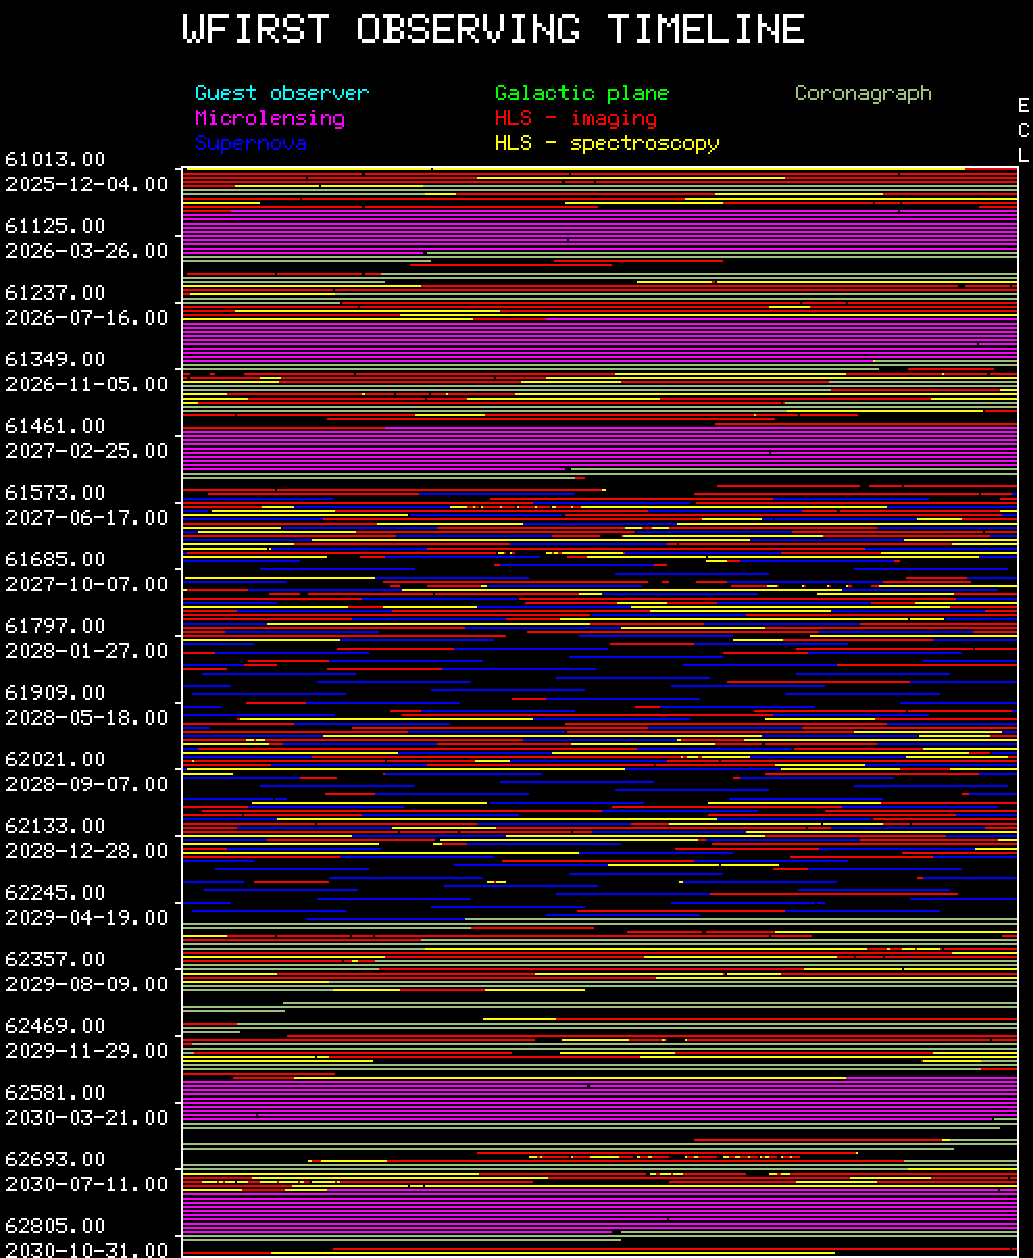
\includegraphics[height=8in]{Plots/observing_chart.pdf}
\caption{\label{fig:observing_chart}Observing timeline. Each row represents 7 days of observations, and is color-coded according to the observing program. Note the microlensing seasons (magenta), supernova survey (blue: $\sim$5-day cadence), and HLS (red+yellow). Blank areas are not allocated. Labels on the left-hand side are shown every 16 weeks.}
\end{figure}

\begin{figure}
\includegraphics[width=5in]{Plots/hlsdepth.pdf}
\caption{\label{fig:hls_depth}The cumulative distribution of HLS exposure depths above a certain area. The pile-up with many exposures at small area is the result of the deep fields.}
\end{figure}

\begin{figure}
\includegraphics[width=5in]{Plots/hlsdust.pdf}
\caption{\label{fig:hls_dust}The cumulative distribution of Galactic dust in the HLS.}
\end{figure}

\begin{figure}
\includegraphics[width=5in]{Plots/hlsbright.pdf}
\caption{\label{fig:hls_bright}The cumulative distribution of zodiacal light in the HLS.}
\end{figure}

\begin{figure}
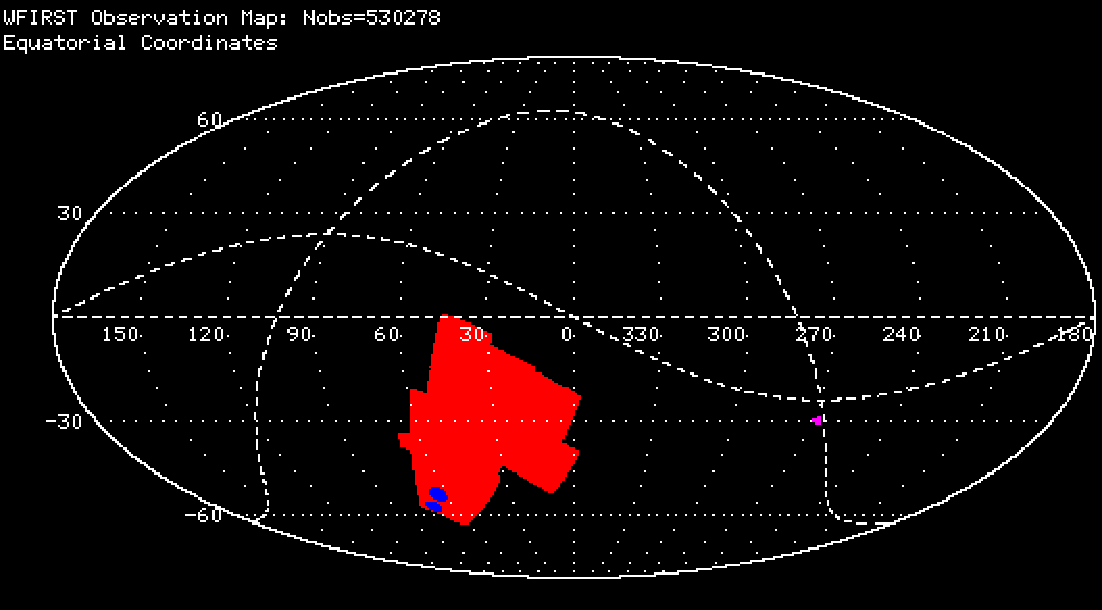
\includegraphics[width=6in]{Plots/sky-equ.pdf}
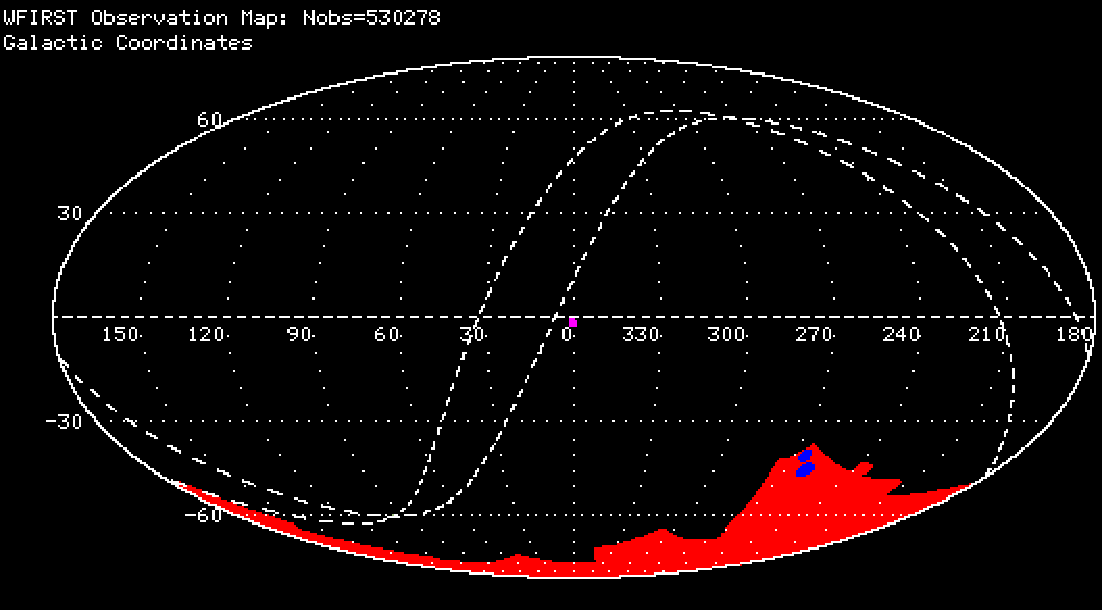
\includegraphics[width=6in]{Plots/sky-gal.pdf}
\caption{\label{fig:footprint}The footprint of the HLS (red) in Equatorial (top) and Galactic (bottom) coordinates.}
\end{figure}

\subsection{Further optimizations}

\begin{summaryii}
Our team plans to study further optimizations to the HLS -- including more
drastic changes such as multi-tiered surveys, or a significant re-balancing of
area vs.\ depth -- in Phase B. However, in preparation for SRR/MDR, our main
focus has been on demonstrating at least one survey configuration that meets
requirements, and the construction of tools that link the observing strategy to
calibration studies (\S\ref{sec:wl_calibration}) and image simulations (\S\ref{sec:hlis_image_sim}).
\end{summaryii}

The optimization of the WFIRST HLS will be tightly linked to operations simulations,
which inform the possible range of footprint area and location, depth in each filter (or grism), redundancy,
and temporal distribution of exposures. We propose a highly integrated approach, with the
operations simulations at the core, but with links to pixel-level simulations to assess required
redundancy, cosmological forecasting tools (\CoLi) to assess science reach, and comparison to the
observing regions of other surveys and telescopes to maximize synergies and meet requirements for
deep fields and photo-$z$ calibration.

% I hope this figure will just be combined with Fig 1.

%
%\setlength\intextsep{-2pt}
%%\begin{center}
%\begin{wrapfigure}{!ht}{0.45\textwidth}
% \begin{boxedminipage}{0.45\textwidth}
% \begin{center}
%\includegraphics[width=1.0\textwidth]{plots/like_DES_WFIRST_combi.eps}
% \end{center}
% \vspace{-1.25cm}
%\caption{{\footnotesize{ \Oli{Initial version for WFIRST vs DES} forecasts multi-probe science case. Probes included are cosmic shear, galaxy clustering, and galaxy-galaxy-lensing from WFIRST (black) in comparison to the Dark Energy Survey (green). The analysis includes BAO, SN1a and Planck information and accounts for galaxy bias, shear calibration, and photo-z errors (with different assumptions for the weak lensing and for the clustering sample). }}}
% \label{tab:milestones}
%\end{boxedminipage}
%\end{wrapfigure}
%% \end{center}
%\setlength\intextsep{0pt}

% \setlength\intextsep{-2pt}
% \begin{wrapfigure}{!ht}{0.75\textwidth}
%  \begin{boxedminipage}{0.75\textwidth}
%  \begin{center}
% \begin{figure*}
% \includegraphics[width=0.5\textwidth]{plots/WFIRST_multi.eps}
%% \caption{\textit{Placeholder plot for WFIRST forecasts multi-probe science case. Probes included are cosmic shear, galaxy clustering, and galaxy-galaxy-lensing, BAO with and without systematics (black and red contours, respectively). The systematics considered in this analysis are shear and photo-z uncertainties (which have different assumptions for the weak lensing and for the clustering sample), and linear galaxy bias. Blue contours include information from DES supernovae type 1a and green contours include an approximate version of Planck CMB temperature and polarization information.}}
%% {\bfseries C.H.: This belongs in another section.}
%%          \label{fi:WFIRST_multi1}
%% \end{figure*}

\subsection{Operations model (D7)}

Co-I Hirata will lead the development of the HLS observing plan,
extending his previous tools used for the SDT. These tools are already
highly advanced, incorporating observing constraints in the candidate
orbits (Geostationary Earth Orbit (GEO) or at the Lagrange point L2),
an exposure-by-exposure observing sequence optimized
with detailed model of overheads, and tiling/coverage maps including
field distortions and curved sky effects. These tools treat both imaging
and spectroscopy with unified functions and scripts, and are well suited to joint survey optimization when
both hardware parameters (e.g., reaction wheel orientations) and the
observing program (e.g., depth vs.\ area) are considered.
Hirata's operations tools were
used by the SDT for ``proof of principle'' studies, but we will now
extend them to (i) evaluate survey performance at intermediate stages
(e.g., what information is available after 1, 2, or 4 years); (ii)
include a pilot survey in the first few months of the mission to
validate HLS performance and make any ``early changes'' necessary;
(iii) include dedicated calibration observations as needed; and (iv)
export field overlap statistics as needed to assess internal calibration
strategies such as ``uber-calibration'' \cite{Padmanabhan2008}. This work will
be performed in consultation with other science groups on the FSWG and with
the WSC.

The SDT coverage maps included a study of the overlap with the LSST footprint,
but with our links to other projects we will understand the overlap with
the other cosmology surveys as well as the accessibility
of our fields from ground-based telescopes. This information, combined with the
community workshops (\S\ref{sec:engagement}), will be used to maximize synergies with
other facilities as well as ensure that potentially conflicting requirements (e.g.,
overlapping LSST photometry and photo-$z$ calibration including Northern telescopes
such as Subaru or Keck) can be met.

%\subsection{Synergies of WFIRST internal probes}
%=====================

%\subsection{Synergies of WFIRST and external data sets}
%=====================

\subsection{Survey Optimization (D10, D11)}
%=================================================
%\Auth{David W, Chris, Olivier}
\label{sec:sur_opt}

%%%%The key constraint in survey optimization is the limited amount of observational time
%%%%available, since WFIRST is life-time limited and has multiple science focus areas.
%%%%For fixed instrumental capabilities and observing time, the most basic
%%%%decision to make about survey strategy is the trade between depth and total area.
%%%%In optimizing the WFIRST WL and BAO/RSD surveys, there are two key considerations:
%%%%(i) {\em precision} -- to maximize the DE science return of WFIRST, taking advantage of synergy with other surveys; and
%%%%(ii) {\em accuracy} -- tight control of systematic uncertainties, to ensure correct DE measurements.
The key constraint in survey optimization is the limited amount of observational time
available, since WFIRST is life-time limited and has multiple science focus areas.
For fixed instrumental capabilities and observing time, the primary
decisions on survey strategy are the trade between depth and total area, and
the balance between imaging and spectroscopy.
These decisions are driven by two major considerations:
(i) {\em precision} -- to maximize the DE science return of WFIRST, taking advantage of synergies with other surveys; and
(ii) {\em accuracy} -- tight control of systematic uncertainties, to ensure correct DE measurements.
The combined expertise of our team in WL and GRS will enable us to rapidly evaluate
these trades, informed by results from previous and concurrent surveys such as
DES/DESI/Euclid. Furthermore, we plan on developing pipelines to
rapidly analyse ``pilot'' data from WFIRST to quantify the telescope
and instrument performance, as well as developing well defined metrics to guide the survey trades.

\subs{WL Survey.} The statistical power of a WL survey scales with the
total number of galaxy shape measurements, the product of the survey area and the effective surface density.
The SDT2015 report adopts an HLS imaging exposure time that yields roughly equal
contributions from read noise and sky noise in the most sensitive
filters, which approximately maximizes the total number of shape
measurements. This is a compromise between minimizing overheads and
read noise (which favors a ``deep'' mode), versus the shallow number
counts of resolved WL sources (shallower than $N\propto F^{-2}$, which
favors a ``wide'' mode). However, we will re-examine the depth vs.\ area trade using
higher-fidelity tools (e.g., incorporation of shape measurement noise from realistic simulations, and updated
detector properties) and propagating the trades all the way to cosmological parameters
(using \CoLi).
We will also investigate the performance of hybrid strategies in
which a four-filter survey over part of the HLS area is combined
with a one- or two-filter survey over a larger area.  This approach
would yield more independent shape measurements at the cost of
greater \photoz\ uncertainties and complicating cross-checks of systematics,
so assessing it requires attention to the entire path from data
to scientific conclusions, including the impacts
on scientific investigations outside of dark energy and cosmological
parameters.

\subs{GRS Survey.} The depth vs.\ area trade for the GRS is driven
by two competing factors: for deep
surveys, where the number density of galaxies $n$ is large ($nP\gg 1$, where $P$ is the power spectrum at
a given scale), the information per unit area saturates; whereas for wide surveys, overheads
reduce inefficiency and galaxy shot noise inflates the statistical errors.
In the SDT15 survey design,
the GRS covers the same area as the HLS imaging survey
($\approx 2,200\deg^2$), to a
$7\sigma$ limiting line flux of $\sim 10^{-16} \erg\cm^{-2}\,{\rm s}^{-1}$
over most of the grism bandpass.
This yields approximately the largest number of galaxy
redshifts for a fixed total observing time.
SDT15 found that doubling the survey area at fixed observing time (even without
additional imaging) {\it reduces} the precision of BAO measurements
because of the rapid increase in galaxy shot noise with decreasing
spectroscopic depth.
However, this conclusion is sensitive to the luminosity function of
H$\alpha$ emitters at $z=1-2$, which remains uncertain \cite{Mehta:2015,Pozzetti:2016};
Co-Is Teplitz and Wang will lead our efforts to reduce this uncertainty
and feed the results into optimization of the GRS.

We will study the link between the observing strategy and systematic error
validation.  For example, pixel-level simulations will predict the variation of
galaxy density with respect to the diversity of roll angles, use of subsets of
the exposures in the data reduction, etc.; our team has extensive experience
with the measurement of such dependences in imaging surveys (Co-Is Ho, Hirata,
Padmanabhan)
and will extend this to the GRS. The hardest part of the GRS error
validation will be galaxy biasing: while it is possible to ``test'' bias models
against a range of simulations with plausible prescriptions for galaxy
placements (HODs, SAMs, etc.), we will ultimately need to validate galaxy
biasing models against the data itself. The most promising avenues are
higher-order statistics (such as 3-point correlations)
and the consistency of results obtained from subsets of the galaxy sample
(e.g., split by magnitude or color).
Both of these demand larger $nP$ and drive
the survey deeper than the power spectrum measurement.
We will develop the tools to assess the precision of these
validation tests and will incorporate them into the survey optimization.

A key consideration in the depth vs.\ area trade is the relation to the Euclid
and DESI redshift surveys; the optimization of WFIRST GRS should avoid portions
of this space that will already be well-explored by these other projects and
focus on the unique capabilities provided by a large telescope in the
low-background space environment.

%Given the assumptions about instrument
%performance and empirical model of the H$\alpha$ luminosity function
%adopted in SDT2015, this exposure time is approximately the one that
%yields the largest number of galaxy redshifts for a fixed total
%In the SDT2015
%survey design, the GRS covers the same area as the HLS imaging survey
%($\approx 2200\deg^2$), and the exposure time of 347 sec yields a
%$7\sigma$ limiting line flux of $\approx 10^{-16} \erg\cm^{-2}\sec^{-1}$
%over most of the grism bandpass.
%
%observing time (0.68 years in SDT2015).
%However, the statistical power
%of a redshift survey does not scale trivially with the number of galaxies,
%and the optimal choice can be quite different for different applications.
%
%The variance in a measurement of the galaxy power spectrum at
%wavenumber $k$ scales inversely with the effective comoving survey volume
%\begin{equation}
%V_{\rm eff}(k) = \int d^3r  [1+nP(k)]^{-1}~,
%\end{equation}
%where $n$ is the galaxy space density.  {\bf Agreed?}
%The optimal tradeoff between depth and area typically occurs
%for $nP = 1-2$; at higher $nP$ it is better to expand the survey
%area to increase volume, while at lower $nP$ it is better to
%go deeper to reduce shot noise.
%SDT2015 forecasts $nP \approx 2-3$ (depending on redshift)
%at the scale $k=0.2\mhmpcinv$
%that is relevant for BAO precision, which suggests that the BAO
%precision could be improved moderately by decreasing the exposure
%time and increasing the survey area; because the survey depth is
%already on the exponential tail of the H$\alpha$ luminosity function,
%the space density drops rapidly with increasing flux limit.
%However, even for the relatively simple case of BAO, optimization
%depends sensitively on instrument characteristics (detector read noise,
%grism throughput, etc.), on the imperfectly known H$\alpha$ and [OIII]
%luminosity functions, on the performance of reconstruction methods,
%and on details of data reduction and incompleteness corrections.
%For example, the methods recently proposed by \cite{suchyta2015}
%could allow effective use of emission line sources down to a $\sim 5\sigma$
%limit, instead of the conservative $7\sigma$ detection threshold assumed by
%SDT2015, and this would significantly shift the optimal exposure time.
%For RSD the optimization depends additionally on the accuracy of theoretical
%techniques to model non-linear galaxy clustering, since this determines
%the maximum wavenumber at which power spectrum measurements are cosmologically
%useful.  We also hope that the methodology investigations described
%above will provide powerful new routes to cosmological parameter constraints
%from higher order clustering measurements, which are more sensitive to
%shot noise.  Relative to power spectrum analyses, these methods likely
%favor a denser survey with higher $nP$, but survey optimization for
%such analyses is largely uncharted territory.

\subs{WFIRST HLS Survey.}  Optimization of the WFIRST HLS requires the end-to-end approach
outlined in this proposal, considering everything from the read noise
of the detectors and contamination of redshift catalogs to the
theoretical modeling systematics for higher order clustering statistics.
It also requires joint consideration of the imaging and spectroscopic
surveys:
multi-filter photometry (as planned in SDT2015) is required to suppress
contaminants in the GRS \cite{Pullen2015}.
We will provide, in addition to our own recommendations,
publicly available tools that can be used by future science teams,
the WFIRST Project, and the community at large to evaluate a variety
of HLS strategies, including changes to the balance between imaging
and spectroscopy.  These tools will enable us and others to incorporate
updated information about instrument and software performance,
empirical data on the galaxy population, progress in modeling techniques,
the expected contributions of other projects like DESI, LSST, and Euclid,
and changes in the experimental dark energy landscape that highlight
the importance of particular classes of measurements.

%}


%\vspace{-0.15in}
%======================================================
\section{Community Engagement and External Data-sets (D11, D12) \Oli{Olivier, 5 pages}}
%======================================================
\label{sec:engagement}
%
% ** SECTION 8 **
%
The coming decade will be an exciting time for cosmology. Before WFIRST launch,  major cosmological imaging surveys (KiDS, HSC, DES) and the DESI and PFS spectroscopic surveys will significantly advance our current understanding. WFIRST, Euclid and LSST  will then go further and survey the sky at optical and infrared wavelengths, the  James Webb Space Telescope (JWST) and the Extremely Large Telescopes (ELTs) will make very deep maps of the sky; eROSITA will survey the X-ray sky; CMB-S4 will make a deep map of the millimeter sky; and the Canadian Hydrogen Intensity Mapping Experiment (CHIME) and other radio surveys will map the large-scale distribution of H$\,${\sc i}.
%
%Our team will explore ways of maximizing the science return from these combined data sets. Our team members are playing significant roles in a number of these projects and have good ties to the other major surveys.
%
One goal of our SIT is to determine the analysis infrastructure and observations needed to achieve the full potential of WFIRST in combination with these  surveys. This is best done through a broad community effort that brings together scientists from these complementary projects. Our SIT team is well-placed to do this, through team members' significant roles in a number of these projects and ties to the other major surveys.

We started to actively engage the community to identify and pursue the key areas where WFIRST and the concurrent projects will provide new opportunities to mitigate systematics and enhance the combined cosmological science return. We started a series of open workshops to study the interplay between major planned surveys and WFIRST into the WFIRST strategy, to identify: (i) pre-launch observations, (ii) how these external data sets affect the WFIRST observing strategy (e.g., deep fields) and the instrument, and (iii) the software needed (to be built post-CDR) for combining these data sets.

The first of this meeting happened in Pasadena on September 2016. It was focused on the synergies between the WFIRST HLS Cosmology SIT and LSST Dark Energy Science Collaboration (DESC), both at the science level but also at the implementation level. The meeting was co-organized by Rachel Bean, Olivier Dor\'e, Steve Kahn and Jason Rhodes and was attended by about 60 scientists from the two collaborations. The slides are available \href{https://conference.ipac.caltech.edu/wfirst_lsst/}{here} and pictures can be seen in Figure~\ref{fig:pic_workshop}. The conclusion of the workshop will be summarized in a white paper to be written shortly.

\begin{figure}
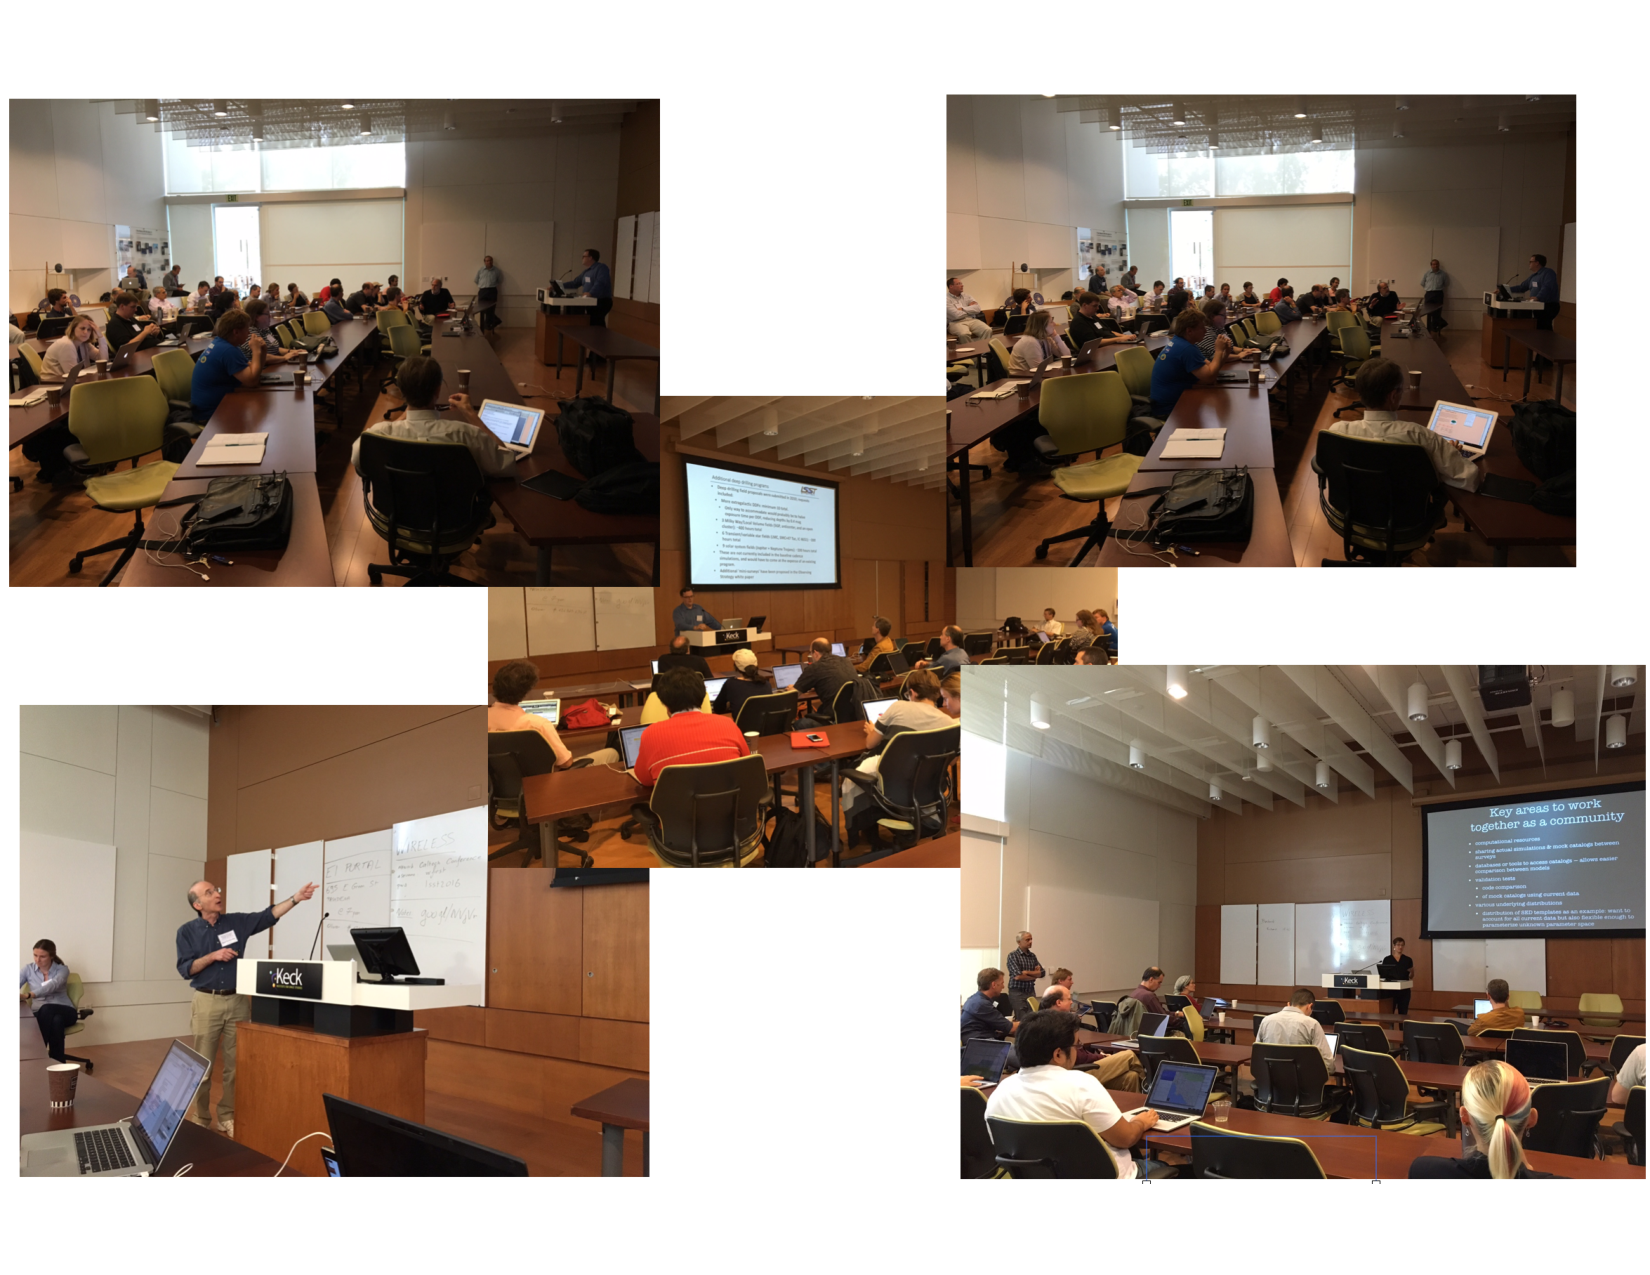
\includegraphics[width=\textwidth,angle=0]{Plots/pic_workshop.pdf}
\caption{\label{fig:pic_workshop}Pictures taken during the Pasadena WFIRST SIT - LSST DESC workshop on September 2016.}
\end{figure}

The workshop was built on the premise that \emph{The Whole is Greater than the
Sum of the Parts: Optimizing the Joint Science Return from LSST, Euclid and
WFIRST} articulated in \citet{Jain:2015cpa}. In the conclusion of this community
white paper, it was articulated that the scientific opportunity offered by the
combination of data from LSST and WFIRST (and Euclid) goes well beyond the
science enabled by any one of the data sets alone. The range in wavelength,
angular resolution and redshift coverage that these missions jointly span is
remarkable. With major investments in LSST and WFIRST (and partnership with ESA
in Euclid), the US has an outstanding scientific opportunity to carry out a
combined analysis of these data sets. It is imperative for us to seize it and,
together with our European colleagues, prepare for the defining cosmological
pursuit of the 21st century.

As illustrated already in \S~\ref{sec:forecast}, the coming decade will be the era of multi-probes/multi-survey science. The richer insights will come from combining multiple probes (WL, GRS, GC) \emph{reliably}. If done properly, multiple survey joint analysis will enable new calibration schemes (photo-$z$, intrinsic alignment models, etc.) and new control of systematics (PSF effects, contaminant control such as stars or interlopers).

The main argument for conducting a single, high-quality reference co-analysis exercise and carefully documenting the results is the complexity and subtlety of systematics that define this co-analysis. Falling back on many small efforts by different teams in selected fields and for narrow goals will be inefficient, leading to significant duplication of effort.  For much of the science, we will need to combine the photometry across multiple wavelengths with varying spectral and spatial resolution – a technical challenge. The joint analysis can be carried out in ways that have different computational demands. The most technically demanding joint analysis is to work with pixel level data of the entire area of overlap between the surveys. Many of the goals of a joint analysis require such a pixel-level analysis. If pixel-level joint analysis is not feasible, catalog-level analysis can still be beneficial, say to obtain calibrations of the lensing shear or the redshift distribution of galaxies. Hybrid efforts are also potentially useful, for example using catalog level information from space for deblending LSST galaxies, or using only a mutually agreed subset of the data for calibration purposes. However the full benefits of jointly analyzing any two of the surveys can be reaped only through pixel-level analysis.

\paragraph{Joint Analysis} In the workshop, possible algorithmic implementation of a joint analysis pipeline were discussed independently by Peter Melchior and Michael Schneider. \citet{Melchior:2016asy} motivated the need for complex morphology models and developed the relevant statistical framework. Complex models become norm. They are more flexible and properly behaved. WFIRST benefits from LSST through color-morphology priors. LSST benefits from sharp likelihood peaks in WFIRST bands. LSST benefits from WFIRST through superior resolution. In HLS directly from a segmentation posterior, otherwise from a prior. \citet{Schneider:2014rha} have developed a probabilistic image reduction pipeline (forward modeling) motivated by challenges in multi-epoch/multi-telescope combinations. They demonstrated improved shear measurements for LSST in the HST Frontier field. 

\paragraph{Ressources} The resources required to achieve this additional science are outside of what is currently budgeted for LSST by NSF and DOE, and for WFIRST (or Euclid) by NASA. Funding for this science would most naturally emerge from coordination among all agencies involved, and would be closely orchestrated scientifically and programmatically to optimize science returns. A possible model would be to identify members of the science teams of each project who would work together on the joint analysis. The analysis team would ideally be coupled with an experienced science center acting as a focal point for the implementation, and simultaneously preparing the public release and documentation for broadest access by the community.
, other interlopers


How can we best take advantage of/combine the efforts from LSST + WFIRST groups working on simulation tools? Photo-z methods?
Communicate and share codes.

What are the requirements for LSST + WFIRST photo-z performance? Or, conversely, what information on photo-z performance do analysis groups need in order to forecast their cosmology constraints and develop pipelines?
More studies are needed.

How do we work together to maximize utility/minimize duplication in spectroscopic samples?
Capak et al. are building a public calibration catalog for WFIRST and LSST.

Relevant also for deep surveys synchronization, discussed in this context and others (SNe, shape cal., grism cal., GO).

Large efforts under way in LSST (DESC) with multiple planned data challenges.
Computational needs:
 Resources available for the scale of simulations required (with possible exception of hydrodynamical simulations).
Infrastructure needs:
Sharing simulations (e.g. Millennium DB) and mock catalogs has greatly 
expanded the use of simulations in a broad range of applications.
A 100 TB to 1 PB scale infrastructure doesn’t exist.
Data transfer will be a challenge (10 days for 100 TB at 1 Gb).
Opportunity for collaborations and investments.
Mock catalogs:
Great progress in the development of mocks from SHAMs, SAMs, hydro
No next generation mock catalogs (or agreement on attributes or what they mean) yet.

Joint analysis will target specific science goals in DE or other areas.  A common-use data legacy from co-processing gets to the science faster and amplifies pay-off well beyond targeted science papers:
Well-designed, well-documented public-release products are best use of limited resources.
They attract new users, enable more science.
Science center expertise can help generate and preserve them efficiently, along with tools, docs, ancillary data, simulations, etc.
“Processing tiers” are one example of resource usage tuned for maximizing the science:
Existing expertise at centers and projects is more than adequate.
This plan is agnostic as to who does what.
Centers and projects do lower tiers, community competes for science exploitation
U.S. agencies and community should be aware of similar planning in Europe, leave open a path to collaboration, but avoid being left behind.
As an aside, LSST project (R. Dubois) estimates that processing WFIRST in the same framework would require ~30-40% additional resources (maybe of by a factor of a few).


Themes we have identified for these multi-experiment workshops include: (i) Statistical methods for next generation cosmological analyses (ii) Strong lensing: synergies between ground and space (iii) Photometric redshift accuracy for next generation surveys (iv) LSST and WFIRST: data simulations and joint analyses to tackle systematics and reveal the dark sector.


Furthermore, through our team's international scientists in Canada and Japan, we plan to also engage these communities in WFIRST science.  If these  countries become partners, we hope that our international co-Investigators will receive support from their agencies and that they will serve as points of contact with their scientific communities and with the CHIME project (Smith) and the Subaru HSC/PFS project (Takada/Yoshida).


The second of this meeting happened in Pasadena on September 2016.


%\vspace{-0.15in}
%======================================================
\section{Future Workplan \Oli{Olivier, all, 5 pages}}
%======================================================
\label{sec:workplan}
%
% ** SECTION 8 **
%

% \setlength\intextsep{-2pt}
% \begin{wrapfigure}{r}{0.5\textwidth}
%  \begin{boxedminipage}{0.5\textwidth}
%  \begin{center}
% \epsfig{file=Plots/team_flow_v1.pdf,angle=0,width=0.99\textwidth}
%  \end{center}
%  \vspace{-0.5cm}
%  \caption{{\footnotesize {Team members commitment to the
%        deliverables listed in \S~\ref{sec:deliverables}. The task lead
%        is in red but for some tasks, we identify separate leaders for
%        WL with a green diamond, GRS with a blue star, and Clusters
%        with a purple triangle.  For D2, we expect Co-I Eifler to
%        take over from PI Dor\'e as overall lead following FY16.}}}
%  \label{tab:flow}
%  \end{boxedminipage}
%  \end{wrapfigure}
%  \setlength\intextsep{0pt}

\subs{Team Management.} We have structured our team to
cover all the areas of expertise required for
the proposed work, and to maximize the synergies between WFIRST
and the cosmology community.
Scientific decisions including the allocation of
funds will be made by the PI in consultation with a Steering
Committee consisting of the PI, the two topic leads (Hirata and Wang),
the topic sub-lead Weinberg plus Spergel, who have extensive organizational experience
through WMAP, ACT, SDSS, National Research Council (NRC) and NASA
committees, and other activities. While the PI will have final authority on these decisions,
this Committee has the mission experience and breadth of knowledge
needed to advise the PI. Monthly Steering
Committee telecons will review the budget and priorities so that our
effort
remains focused on the scientific success of WFIRST.
Each topic lead will report to the PI on a monthly basis, to facilitate monitoring
of all team work, enable advice on budget priorities, and ensure a
regular review of work effort. The PI will ensure proper
communication with the WFIRST program office and will maximize
collaborations with other WFIRST SITs. For
example, we anticipate jointly developing and sharing low-level image
simulation tools with SN-focused SITs. Topic leads will closely
monitor the progress of the technical tasks (listed in
\S\S~\ref{sec:deliverables},\ref{sec:wl_gal-clusters},\ref{sec:gc}) in
association with the deliverables and will adjust the scope of the
work according to developments in the project and in the field.

\subs{Risk Management.} Inefficient collaboration/coordination presents
the most significant risk for accomplishing our program. Within our
 SIT, this is mitigated partly by most Co-Is having experience
working together in existing (or past) projects. The PI will
coordinate the team's effort, and ensure it is well-integrated into
and aligned with the broader WFIRST effort. The PI will lead the following:
%  to ensure a productive, harmonious, and coordinated collaboration. (1) the PI will
(i)  Monthly telecons with the Steering Committee, to optimize the team effort; (ii)
Regular telecons with all team members, with status updates
from the deliverables leads (Fig.~\ref{tab:flow}) so that progress, issues, and
solutions are broadly visible across the team. (iii) Yearly face-to-face
meetings and more focused working meetings will be added as
needed (the associated travel costs have been
budgeted). Monthly, the Steering Committee will evaluate progress
reports and redistribute responsibilities within the team if
necessary. Finally, team members will present %(in person or remotely)
recent progress, results, and goals for the upcoming year to
an external review panel at this annual meeting. This will also serve as a NASA management
review with representatives of NASA HQ and the JPL WFIRST Project
Office invited to attend. This follows the successful model used by
the US Planck and US Euclid teams with which the PI and many Co-Is have
experience. The PI will also set-up wikis and repositories for efficient
sharing and discussion of software, documents, plans, progress and
issues. We plan to share with the community the software developed for
this program. Key results will be published in peer review papers.

\subs{Program Milestones.} In Fig.~\ref{tab:milestones_mgt} we outline milestones for
our effort in conjunction with the
\setlength\intextsep{-2pt}
%\begin{center}
%\begin{wrapfigure}{r}{0.75\textwidth}
% \begin{boxedminipage}{0.75\textwidth}
% \begin{center}
%\epsfig{file=Plots/wfirst_milestones_v2.pdf,angle=0,width=0.99\textwidth}
% \end{center}
% \vspace{-0.5cm}
% \caption{{\footnotesize Our deliverable schedule in concordance with the
%       WFIRST project timeline as displayed in the WFIRST SIT call \S
%       3.2. Deliverables that are made in multiple stages are labeled
%       (a, b and c) and appear in multiple years.}}
% \label{tab:milestones_mgt}
% \end{boxedminipage}
% \end{wrapfigure}
%\end{center}
%\setlength\intextsep{0pt}
project timeline.

\subs{Postdocs and Students.}  The largest component of our budget is support for postdoctoral researchers
who will work under the supervision of the PI and Co-Is to carry out the
many calculations, simulations, and tests needed to accomplish our
tasks.  Our budget incorporates an initial plan for which postdocs will
be located at which institutions in which years to work on which tasks.

However, the optimal division of labor may shift over time, and the
Steering Committee will consider reallocations of work annually
based on internal proposals from team members.  Where appropriate,
we will consider raising collaborators to funded Co-Is, with NASA approval,
if they are best positioned to carry out particular tasks.
Many of the methodology development efforts, and some of the
technical tasks, are well suited to graduate students, supported
by other sources or by this Investigation if their work
clearly falls within its scope.  In addition to accomplishing the
work of this proposal, the involvement of many postdocs and students
will build a cadre of young researchers who are ideally positioned
to exploit the scientific opportunities of WFIRST.

\subs{A Unified Team.} As is evident from our previous discussion, jointly addressing the
weak lensing and redshift-space clustering elements of the WFIRST
dark energy program leads to an ambitious task list that offers critical
advantages relative to studying them separately.  First is the effective use of expertise; many members of
our team have expertise in both of these program elements and will
contribute to both during the course of this investigation. Second is
the commonality of the hardware; HLS Imaging and Spectroscopy use the
same telescope, detectors, and data systems, and it makes sense to develop associated requirements
through joint consideration of the two surveys.
Third is the need to develop a unified operations concept for these
two interleaved surveys; in overall footprint and in details of
dither patterns and roll angles, choices made for one survey affect
the performance of the other.

Finally, a joint investigation allows us to take a broad perspective
on the WFIRST dark energy program, including a common forecasting
framework that can account for complementary information and the
ability of one survey to mitigate systematics in the other,
common sets of cosmological simulations and models of galaxy bias
that are relevant to both topics, and investigation of trades
between HLS Imaging and Spectroscopy.  We have carefully
constructed a team capable of addressing all of the essential tasks for elements A and C of the WFIRST SIT NRA, and
we have requested resources that will enable us to accomplish this work.
If NASA decides to select additional teams in these areas we will be glad to collaborate with them.
As emphasized in \S\ref{sec:engagement}, WFIRST is a national and international resource, and
it is valuable to engage as much of the astronomical community
as possible in its formulation.


\clearpage
\newpage

%===============
%\section{References}

%=========================
\section*{ACKNOWLEDGMENTS}
%=========================
\label{sec:acknowledgments}
%\addcontentsline{toc}{section}{ACKNOWLEDGMENTS}
% Section acknowledgement

We warmly thank our colleagues from the WFIRST project office and all the Science Investigation Teams for continuous and constructive interactions. We acknowledge use of the Annual Review of Astronomy and Astrophysics LaTeX template as a basis for our report. Part of this research was carried out at the Jet Propulsion Laboratory, California Institute of Technology, under a contract with the National Aeronautics and Space Administration.


%===============
\section{List of Acronyms and Abbreviations and References}
%===============
%\addcontentsline{toc}{section}{References and List of Acronyms and Abbreviations}
\label{sec:acronyms}

\begin{table*}[ht!]
  \small
  \begin{tabular}{@{}>{\raggedright}p{0.085\textwidth}>{\raggedright}p{0.39\textwidth}>{\raggedright}p{0.085\textwidth}>{\raggedright}p{0.39\textwidth}}

    $\sigma_m$ & -- rms amplitude of matter fluctuations
    & LSS & -- large scale structure \tabularnewline
    $\Omega_m$ & -- dimensionless density of the Universe
    & LSST & -- Large Synoptic Survey Telescope \tabularnewline
    $a$ \\ ACT & -- scale-factor of the Universe \\ -- Atacama Cosmology
    Telescope
    & NICMOS & -- HST Near Infrared Camera and Multi-Object Spectrometer
    \tabularnewline
    AdvACT & -- Advanced ACT
    & NIR & -- near-infrared \tabularnewline
    AFTA & -- Astrophysics Focused Telescope Asset
    & NRA & -- NASA Research Announcement \tabularnewline
    BAO & -- baryon acoustic oscillations
    & NRC & -- National Research Council \tabularnewline
    BOSS & -- Baryon Oscillation Spectroscopic Survey
    & NWNH \\ $P_m$ & -- New Worlds, New Horizons \\ -- matter power spectrum
    \tabularnewline
    CDR & -- critical design review
    & PFS & -- Subaru Prime Focus Spectrograph \tabularnewline
    CFHT & -- Canada-France-Hawaii Telescope
    & photo-$z$ & -- photometric redshift \tabularnewline
    CGL & -- cluster-galaxy lensing
    & PSF & -- point spread function \tabularnewline
    CHIME & -- Canadian Hydrogen Intensity Mapping Experiment
    & RSD \\ SAM & -- redshift-space distortions \\
    -- semi-analytic galaxy formation models \tabularnewline
    CL & -- galaxy clusters / cluster growth
    & SDSS & -- Sloan Digital Sky Survey \tabularnewline
    CMB & -- cosmic microwave background
    & SDT & -- Science Definition Team \tabularnewline
    CMB-S4 & -- CMB stage 4 experiment
    & SDT13 & -- 2013 WFIRST SDT report \tabularnewline
    $D(z)$ & -- distance-redshift relation
    & SDT15 & -- 2015 WFIRST SDT report \tabularnewline
    $D_A(z)$ & -- angular-diameter distance
    & SIT & -- Science Investigation Team \tabularnewline
    DE & -- dark energy
    & SMEX & -- NASA Small Explorer \tabularnewline
    DES & -- Dark Energy Survey
    & SN & -- supernovae \tabularnewline
    DESC & -- Dark Energy Science Collaboration
    & S/N & -- signal-to-noise \tabularnewline
    DESI \\ ELG \\ ELTs & -- Dark Energy Spectroscopic Instrument \\
    -- emission line galaxies \\ -- Extremely Large Telescopes
    & SPHEREx & -- Spectrophotometer for the History of the Universe, Epoch of
    Reionization, and Ices Explorer\tabularnewline
    eROSITA & -- extended Roentgen Survey with an Imaging Telescope Array
    & SPT-3G & -- South Pole Telescope Third-Generation Camera Survey
    \tabularnewline
    ETC & -- Exposure Time Calculator
    & STEP & -- Shear Testing Program \tabularnewline
    $f_g$ \\ FSWG & -- fluctuation growth rate \\ -- Formulation Science
    Working Group
    & STIS & HST Space Telescope Imaging Spectrograph \tabularnewline
    GEO & -- geostationary earth orbit
    & SZ & -- Sunyaev-Zeldovich \tabularnewline
    GGL & -- galaxy-galaxy lensing
    & $w(z)$ & -- dark energy equation-of-state \tabularnewline
    GREAT & -- Gravitational Lensing Accuracy Test
    & WFC3 & HST Wide-Field Camera 3 \tabularnewline
    GREAT3 & -- The third GREAT challenge
    & WFIRST & -- Wide-Field Infrared Survey Telescope \tabularnewline
    GRS \\ $H(z)$ & -- Galaxy Redshift Survey \\ -- Hubble parameter
    & WISPs & -- HST WFC3 IR Spectroscopic Parallel survey \tabularnewline
    HLS & -- High Latitude Survey
    & WL & -- weak lensing  \tabularnewline
    HOD & -- halo occupation distribution
    & WMAP & -- Wilkinson Microwave Anisotropy Probe \tabularnewline
    HSC & -- Subaru Hyper Suprime-Cam
    & WPS & -- WFIRST Preparatory Science \tabularnewline
    HST & -- Hubble Space Telescope
    & WSC & -- WFIRST Science Centers \tabularnewline
    IA & -- intrinsic galaxy alignments
    & $z$ & -- redshift \tabularnewline
    IPAC & -- Infrared Processing and Analysis Center
    & $z_p$ & -- pivot redshift \tabularnewline
    IPC & -- inter-pixel capacitance
    & & \tabularnewline
    IR & -- infrared
    & & \tabularnewline
    JDEM & -- Joint Dark Energy Mission
    & & \tabularnewline
    JWST & -- James Webb Space Telescope
    & & \tabularnewline
    KiDS & -- Kilo Degree Survey
    & & \tabularnewline
    L2 & -- Lagrange point 2 orbit
    & & \tabularnewline
    LF & -- luminosity function
    & & \tabularnewline

    
  \end{tabular}
\end{table*}





\clearpage
\newpage

%\addcontentsline{toc}{section}{References}

We highlighted in bold the team members in the following bibliography.

\bibliographystyle{abbrv}
\bibliography{refs}

\clearpage
\newpage

\end{document}
